\documentclass[oneside]{book}
%---------------------------Packages----------------------------%
\usepackage{geometry}
\geometry{b5paper, margin=1.0in}
\usepackage[T1]{fontenc}
\usepackage{graphicx, float}            % Graphics/Images.
\usepackage{natbib}                     % For bibliographies.
\bibliographystyle{agsm}                % Bibliography style.
\usepackage[french, english]{babel}     % Language typesetting.
\usepackage[dvipsnames]{xcolor}         % Color names.
\usepackage{listings}                   % Verbatim-Like Tools.
\usepackage{mathtools, esint, mathrsfs} % amsmath and integrals.
\usepackage{amsthm, amsfonts, amssymb}  % Fonts and theorems.
\usepackage{tcolorbox}                  % Frames around theorems.
\usepackage{upgreek}                    % Non-Italic Greek.
\usepackage{fmtcount, etoolbox}         % For the \book{} command.
\usepackage[newparttoc]{titlesec}       % Formatting chapter, etc.
\usepackage{titletoc}                   % Allows \book in toc.
\usepackage[nottoc]{tocbibind}          % Bibliography in toc.
\usepackage[titles]{tocloft}            % ToC formatting.
\usepackage{pgfplots, tikz}             % Drawing/graphing tools.
\usepackage{imakeidx}                   % Used for index.
\usetikzlibrary{
    calc,                   % Calculating right angles and more.
    angles,                 % Drawing angles within triangles.
    arrows.meta,            % Latex and Stealth arrows.
    quotes,                 % Adding labels to angles.
    positioning,            % Relative positioning of nodes.
    decorations.markings,   % Adding arrows in the middle of a line.
    patterns,
    arrows
}                                       % Libraries for tikz.
\pgfplotsset{compat=1.9}                % Version of pgfplots.
\usepackage[font=scriptsize,
            labelformat=simple,
            labelsep=colon]{subcaption} % Subfigure captions.
\usepackage[font={scriptsize},
            hypcap=true,
            labelsep=colon]{caption}    % Figure captions.
\usepackage[pdftex,
            pdfauthor={Ryan Maguire},
            pdftitle={Mathematics and Physics},
            pdfsubject={Mathematics, Physics, Science},
            pdfkeywords={Mathematics, Physics, Computer Science, Biology},
            pdfproducer={LaTeX},
            pdfcreator={pdflatex}]{hyperref}
\hypersetup{
    colorlinks=true,
    linkcolor=blue,
    filecolor=magenta,
    urlcolor=Cerulean,
    citecolor=SkyBlue
}                           % Colors for hyperref.
\usepackage[toc,acronym,nogroupskip,nopostdot]{glossaries}
\usepackage{glossary-mcols}
%------------------------Theorem Styles-------------------------%
\theoremstyle{plain}
\newtheorem{theorem}{Theorem}[section]

% Define theorem style for default spacing and normal font.
\newtheoremstyle{normal}
    {\topsep}               % Amount of space above the theorem.
    {\topsep}               % Amount of space below the theorem.
    {}                      % Font used for body of theorem.
    {}                      % Measure of space to indent.
    {\bfseries}             % Font of the header of the theorem.
    {}                      % Punctuation between head and body.
    {.5em}                  % Space after theorem head.
    {}

% Italic header environment.
\newtheoremstyle{thmit}{\topsep}{\topsep}{}{}{\itshape}{}{0.5em}{}

% Define environments with italic headers.
\theoremstyle{thmit}
\newtheorem*{solution}{Solution}

% Define default environments.
\theoremstyle{normal}
\newtheorem{example}{Example}[section]
\newtheorem{definition}{Definition}[section]
\newtheorem{problem}{Problem}[section]

% Define framed environment.
\tcbuselibrary{most}
\newtcbtheorem[use counter*=theorem]{ftheorem}{Theorem}{%
    before=\par\vspace{2ex},
    boxsep=0.5\topsep,
    after=\par\vspace{2ex},
    colback=green!5,
    colframe=green!35!black,
    fonttitle=\bfseries\upshape%
}{thm}

\newtcbtheorem[auto counter, number within=section]{faxiom}{Axiom}{%
    before=\par\vspace{2ex},
    boxsep=0.5\topsep,
    after=\par\vspace{2ex},
    colback=Apricot!5,
    colframe=Apricot!35!black,
    fonttitle=\bfseries\upshape%
}{ax}

\newtcbtheorem[use counter*=definition]{fdefinition}{Definition}{%
    before=\par\vspace{2ex},
    boxsep=0.5\topsep,
    after=\par\vspace{2ex},
    colback=blue!5!white,
    colframe=blue!75!black,
    fonttitle=\bfseries\upshape%
}{def}

\newtcbtheorem[use counter*=example]{fexample}{Example}{%
    before=\par\vspace{2ex},
    boxsep=0.5\topsep,
    after=\par\vspace{2ex},
    colback=red!5!white,
    colframe=red!75!black,
    fonttitle=\bfseries\upshape%
}{ex}

\newtcbtheorem[auto counter, number within=section]{fnotation}{Notation}{%
    before=\par\vspace{2ex},
    boxsep=0.5\topsep,
    after=\par\vspace{2ex},
    colback=SeaGreen!5!white,
    colframe=SeaGreen!75!black,
    fonttitle=\bfseries\upshape%
}{not}

\newtcbtheorem[use counter*=remark]{fremark}{Remark}{%
    fonttitle=\bfseries\upshape,
    colback=Goldenrod!5!white,
    colframe=Goldenrod!75!black}{ex}

\newenvironment{bproof}{\textit{Proof.}}{\hfill$\square$}
\tcolorboxenvironment{bproof}{%
    blanker,
    breakable,
    left=3mm,
    before skip=5pt,
    after skip=10pt,
    borderline west={0.6mm}{0pt}{green!80!black}
}

\AtEndEnvironment{lexample}{$\hfill\textcolor{red}{\blacksquare}$}
\newtcbtheorem[use counter*=example]{lexample}{Example}{%
    empty,
    title={Example~\theexample},
    boxed title style={%
        empty,
        size=minimal,
        toprule=2pt,
        top=0.5\topsep,
    },
    coltitle=red,
    fonttitle=\bfseries,
    parbox=false,
    boxsep=0pt,
    before=\par\vspace{2ex},
    left=0pt,
    right=0pt,
    top=3ex,
    bottom=1ex,
    before=\par\vspace{2ex},
    after=\par\vspace{2ex},
    breakable,
    pad at break*=0mm,
    vfill before first,
    overlay unbroken={%
        \draw[red, line width=2pt]
            ([yshift=-1.2ex]title.south-|frame.west) to
            ([yshift=-1.2ex]title.south-|frame.east);
        },
    overlay first={%
        \draw[red, line width=2pt]
            ([yshift=-1.2ex]title.south-|frame.west) to
            ([yshift=-1.2ex]title.south-|frame.east);
    },
}{ex}

\AtEndEnvironment{ldefinition}{$\hfill\textcolor{Blue}{\blacksquare}$}
\newtcbtheorem[use counter*=definition]{ldefinition}{Definition}{%
    empty,
    title={Definition~\thedefinition:~{#1}},
    boxed title style={%
        empty,
        size=minimal,
        toprule=2pt,
        top=0.5\topsep,
    },
    coltitle=Blue,
    fonttitle=\bfseries,
    parbox=false,
    boxsep=0pt,
    before=\par\vspace{2ex},
    left=0pt,
    right=0pt,
    top=3ex,
    bottom=0pt,
    before=\par\vspace{2ex},
    after=\par\vspace{1ex},
    breakable,
    pad at break*=0mm,
    vfill before first,
    overlay unbroken={%
        \draw[Blue, line width=2pt]
            ([yshift=-1.2ex]title.south-|frame.west) to
            ([yshift=-1.2ex]title.south-|frame.east);
        },
    overlay first={%
        \draw[Blue, line width=2pt]
            ([yshift=-1.2ex]title.south-|frame.west) to
            ([yshift=-1.2ex]title.south-|frame.east);
    },
}{def}

\AtEndEnvironment{ltheorem}{$\hfill\textcolor{Green}{\blacksquare}$}
\newtcbtheorem[use counter*=theorem]{ltheorem}{Theorem}{%
    empty,
    title={Theorem~\thetheorem:~{#1}},
    boxed title style={%
        empty,
        size=minimal,
        toprule=2pt,
        top=0.5\topsep,
    },
    coltitle=Green,
    fonttitle=\bfseries,
    parbox=false,
    boxsep=0pt,
    before=\par\vspace{2ex},
    left=0pt,
    right=0pt,
    top=3ex,
    bottom=-1.5ex,
    breakable,
    pad at break*=0mm,
    vfill before first,
    overlay unbroken={%
        \draw[Green, line width=2pt]
            ([yshift=-1.2ex]title.south-|frame.west) to
            ([yshift=-1.2ex]title.south-|frame.east);},
    overlay first={%
        \draw[Green, line width=2pt]
            ([yshift=-1.2ex]title.south-|frame.west) to
            ([yshift=-1.2ex]title.south-|frame.east);
    }
}{thm}

%--------------------Declared Math Operators--------------------%
\DeclareMathOperator{\adjoint}{adj}         % Adjoint.
\DeclareMathOperator{\Card}{Card}           % Cardinality.
\DeclareMathOperator{\curl}{curl}           % Curl.
\DeclareMathOperator{\diam}{diam}           % Diameter.
\DeclareMathOperator{\dist}{dist}           % Distance.
\DeclareMathOperator{\Div}{div}             % Divergence.
\DeclareMathOperator{\Erf}{Erf}             % Error Function.
\DeclareMathOperator{\Erfc}{Erfc}           % Complementary Error Function.
\DeclareMathOperator{\Ext}{Ext}             % Exterior.
\DeclareMathOperator{\GCD}{GCD}             % Greatest common denominator.
\DeclareMathOperator{\grad}{grad}           % Gradient
\DeclareMathOperator{\Ima}{Im}              % Image.
\DeclareMathOperator{\Int}{Int}             % Interior.
\DeclareMathOperator{\LC}{LC}               % Leading coefficient.
\DeclareMathOperator{\LCM}{LCM}             % Least common multiple.
\DeclareMathOperator{\LM}{LM}               % Leading monomial.
\DeclareMathOperator{\LT}{LT}               % Leading term.
\DeclareMathOperator{\Mod}{mod}             % Modulus.
\DeclareMathOperator{\Mon}{Mon}             % Monomial.
\DeclareMathOperator{\multideg}{mutlideg}   % Multi-Degree (Graphs).
\DeclareMathOperator{\nul}{nul}             % Null space of operator.
\DeclareMathOperator{\Ord}{Ord}             % Ordinal of ordered set.
\DeclareMathOperator{\Prin}{Prin}           % Principal value.
\DeclareMathOperator{\proj}{proj}           % Projection.
\DeclareMathOperator{\Refl}{Refl}           % Reflection operator.
\DeclareMathOperator{\rk}{rk}               % Rank of operator.
\DeclareMathOperator{\sgn}{sgn}             % Sign of a number.
\DeclareMathOperator{\sinc}{sinc}           % Sinc function.
\DeclareMathOperator{\Span}{Span}           % Span of a set.
\DeclareMathOperator{\Spec}{Spec}           % Spectrum.
\DeclareMathOperator{\supp}{supp}           % Support
\DeclareMathOperator{\Tr}{Tr}               % Trace of matrix.
%--------------------Declared Math Symbols--------------------%
\DeclareMathSymbol{\minus}{\mathbin}{AMSa}{"39} % Unary minus sign.
%------------------------New Commands---------------------------%
\DeclarePairedDelimiter\norm{\lVert}{\rVert}
\DeclarePairedDelimiter\ceil{\lceil}{\rceil}
\DeclarePairedDelimiter\floor{\lfloor}{\rfloor}
\newcommand*\diff{\mathop{}\!\mathrm{d}}
\newcommand*\Diff[1]{\mathop{}\!\mathrm{d^#1}}
\renewcommand*{\glstextformat}[1]{\textcolor{RoyalBlue}{#1}}
\renewcommand{\glsnamefont}[1]{\textbf{#1}}
\renewcommand\labelitemii{$\circ$}
\renewcommand\thesubfigure{%
    \arabic{chapter}.\arabic{figure}.\arabic{subfigure}}
\addto\captionsenglish{\renewcommand{\figurename}{Fig.}}
\numberwithin{equation}{section}

\renewcommand{\vector}[1]{\boldsymbol{\mathrm{#1}}}

\newcommand{\uvector}[1]{\boldsymbol{\hat{\mathrm{#1}}}}
\newcommand{\topspace}[2][]{(#2,\tau_{#1})}
\newcommand{\measurespace}[2][]{(#2,\varSigma_{#1},\mu_{#1})}
\newcommand{\measurablespace}[2][]{(#2,\varSigma_{#1})}
\newcommand{\manifold}[2][]{(#2,\tau_{#1},\mathcal{A}_{#1})}
\newcommand{\tanspace}[2]{T_{#1}{#2}}
\newcommand{\cotanspace}[2]{T_{#1}^{*}{#2}}
\newcommand{\Ckspace}[3][\mathbb{R}]{C^{#2}(#3,#1)}
\newcommand{\funcspace}[2][\mathbb{R}]{\mathcal{F}(#2,#1)}
\newcommand{\smoothvecf}[1]{\mathfrak{X}(#1)}
\newcommand{\smoothonef}[1]{\mathfrak{X}^{*}(#1)}
\newcommand{\bracket}[2]{[#1,#2]}

%------------------------Book Command---------------------------%
\makeatletter
\renewcommand\@pnumwidth{1cm}
\newcounter{book}
\renewcommand\thebook{\@Roman\c@book}
\newcommand\book{%
    \if@openright
        \cleardoublepage
    \else
        \clearpage
    \fi
    \thispagestyle{plain}%
    \if@twocolumn
        \onecolumn
        \@tempswatrue
    \else
        \@tempswafalse
    \fi
    \null\vfil
    \secdef\@book\@sbook
}
\def\@book[#1]#2{%
    \refstepcounter{book}
    \addcontentsline{toc}{book}{\bookname\ \thebook:\hspace{1em}#1}
    \markboth{}{}
    {\centering
     \interlinepenalty\@M
     \normalfont
     \huge\bfseries\bookname\nobreakspace\thebook
     \par
     \vskip 20\p@
     \Huge\bfseries#2\par}%
    \@endbook}
\def\@sbook#1{%
    {\centering
     \interlinepenalty \@M
     \normalfont
     \Huge\bfseries#1\par}%
    \@endbook}
\def\@endbook{
    \vfil\newpage
        \if@twoside
            \if@openright
                \null
                \thispagestyle{empty}%
                \newpage
            \fi
        \fi
        \if@tempswa
            \twocolumn
        \fi
}
\newcommand*\l@book[2]{%
    \ifnum\c@tocdepth >-3\relax
        \addpenalty{-\@highpenalty}%
        \addvspace{2.25em\@plus\p@}%
        \setlength\@tempdima{3em}%
        \begingroup
            \parindent\z@\rightskip\@pnumwidth
            \parfillskip -\@pnumwidth
            {
                \leavevmode
                \Large\bfseries#1\hfill\hb@xt@\@pnumwidth{\hss#2}
            }
            \par
            \nobreak
            \global\@nobreaktrue
            \everypar{\global\@nobreakfalse\everypar{}}%
        \endgroup
    \fi}
\newcommand\bookname{Book}
\renewcommand{\thebook}{\texorpdfstring{\Numberstring{book}}{book}}
\providecommand*{\toclevel@book}{-2}
\makeatother
\titleformat{\part}[display]
    {\Large\bfseries}
    {\partname\nobreakspace\thepart}
    {0mm}
    {\Huge\bfseries}
\titlecontents{part}[0pt]
    {\large\bfseries}
    {\partname\ \thecontentslabel: \quad}
    {}
    {\hfill\contentspage}
\titlecontents{chapter}[0pt]
    {\bfseries}
    {\chaptername\ \thecontentslabel:\quad}
    {}
    {\hfill\contentspage}
\newglossarystyle{longpara}{%
    \setglossarystyle{long}%
    \renewenvironment{theglossary}{%
        \begin{longtable}[l]{{p{0.25\hsize}p{0.65\hsize}}}
    }{\end{longtable}}%
    \renewcommand{\glossentry}[2]{%
        \glstarget{##1}{\glossentryname{##1}}%
        &\glossentrydesc{##1}{~##2.}
        \tabularnewline%
        \tabularnewline
    }%
}
\newglossary[not-glg]{notation}{not-gls}{not-glo}{Notation}
\newcommand*{\newnotation}[4][]{%
    \newglossaryentry{#2}{type=notation, name={\textbf{#3}, },
                          text={#4}, description={#4},#1}%
}
%--------------------------LENGTHS------------------------------%
% Spacings for the Table of Contents.
\addtolength{\cftsecnumwidth}{1ex}
\addtolength{\cftsubsecindent}{1ex}
\addtolength{\cftsubsecnumwidth}{1ex}
\addtolength{\cftfignumwidth}{1ex}
\addtolength{\cfttabnumwidth}{1ex}

% Indent and paragraph spacing.
\setlength{\parindent}{0em}
\setlength{\parskip}{0em}
\makeglossaries
\loadglsentries{glossary}
\loadglsentries{acronym}
\begin{document}
    \title{Diffraction Through Planetary Rings}
    \author{Ryan Maguire}
    \date{\vspace{-5ex}}
    \pagenumbering{roman}
    \maketitle
    \tableofcontents
    \listoffigures
    \listoftables
    \clearpage
    \chapter*{Preface}
\addcontentsline{toc}{chapter}{Preface}
    This book was written to provide a student of physics the material
    needed to independently study the radio occultation observations that
    have been made by both the Voyager and Cassini radio science missions.
    In developing the mathematics necessary for diffraction theory, it is
    foolishly assumed that the reader has a strong
    familiarity with differential and integral calculus, and is aware of the
    $\varepsilon-\delta$ definition of continuity. An attempt was made to
    make this the only prerequesite, and the first (And longest) chapter
    is entirely devoted to developing mathematics. This chapter covers
    complex, Fourier, and numerical analysis, as well as partial
    differential equations and bits of vector calculus. No effort was made
    to shy away from rigor, and proofs of almost all theorems are given.
    It is not the author's wish to present mathematics as a list of
    mysterious formulae with no background.
    \par\hfill\par
    Those familiar with the preliminaries may skip chapter 1, but this is
    discouraged. Many counter-intuitive results from the theory of
    integration and of distributions will be presented, and the
    derivations made in later chapters make constant reference to the
    theorems proved here. The second chapter derives the Fresnel-Huygens
    principle, taking the Maxwell Equations as the axioms of
    electromagnetism. No previous experience with electricity and magnetism
    is expected, but will make understanding the derivations easier.
    But indeed, in a course on electromagnetism one often takes
    \textit{Coulomb's Law} and the \textit{Biot-Savart Law} as axioms,
    on the basis of experimental data, and from there derives Maxwell's
    equations. It is perfectly valid to go on the other direction as well.
    \par\hfill\par
    The Third and Fourth chapters are dedicated to diffraction in the
    context of occultation observations of planetary rings. The geometries
    of such experiments are presented, and the numerical methods we'll
    develop are used to justify various approximations for
    reconstructing ring profiles from the diffraction limited data.
    \par\hfill\par
    Part II of this books pertains to applying the theory to the Cassini
    radio science mission, and analyzes the rings of Saturn. Various
    algorithms are presented, and routines in the C programming language
    are given. This part will also demonstrate the limitations of the
    approximations, and the need for careful analysis.
    \par\hfill\par
    \hfill
    Ryan Maguire
    \par\hfill
    Wellesley College
    \par\hfill
    August, 2019
    \clearpage
    \pagenumbering{arabic}
    \part{Preliminaries}
        We begin with a few important topics in mathematics that one comes
across in the study of electromagnetism and diffraction theory.
This is particularly useful for studying occultation observations
of planetary rings. We will develop complex analysis, Fourier analysis,
approximation theory, and multivariate calculus so that we may
transition from the core of electromagnetism, \textit{Maxwell's Equations},
and derive the \textit{Fresnel-Huygens Principle}. This is the fundamental
equation on which diffraction theory is based.
\par\hfill\par
There is a standard set of notations in mathematics, and this is
presented below in Table~\ref{tab:Common_Notations}.
\begin{table}[H]
    \centering
    \captionsetup{type=table}
    \begin{tabular}{|l|l|}
        \hline
        Symbol&Definition\\
        \hline
        $\mathbb{N}$&Positive Integers\\
        \hline
        $\mathbb{Z}$&Integers\\
        \hline
        $\mathbb{Z}_{n}$&Positive Integers Between 1 and $n$.\\
        \hline
        $\mathbb{Q}$&Rational numbers\\
        \hline
        $\mathbb{R}$&Real Numbers\\
        \hline
        $\mathbb{C}$&Complex Numbers\\
        \hline
    \end{tabular}
    \caption{Common Notations}
    \label{tab:Common_Notations}
\end{table}
Given some number $x$, we denote that $x$ is a real number by writing
$x\in\mathbb{R}$, and similarly if $x$ is rational we write
$x\in\mathbb{Q}$. Conversely, we write $x\notin\mathbb{R}$ to denote that
$x$ is \textit{not} a real number. The $\in$ symbol should be read
\textit{is an element of}, so $x\in\mathbb{R}$ reads as $x$
\textit{is an element of} $\mathbb{R}$. Recall that a
\textit{sequence} of points in some set $A$ is an ordered list
$a_{1}$, $a_{2}$, $\dots$, $a_{n}$, $\dots$ such that $a_{k}\in{A}$
for all $k\in\mathbb{N}$. This definition lacks rigor in many
respects, and to make the notion useful we define a sequence as
a \textit{function} from $\mathbb{N}$ to $A$. That is, we write
$a:\mathbb{N}\rightarrow{A}$. Rather than writing $a(n)$, we write
$a_{n}$. Subscript notation is reserved for sequences. For a
general function $f:X\rightarrow{Y}$, we
write $f(x)$ to denote the point in $Y$ that corresponds to $x$.

        \chapter{Complex Analysis}
    The theory of complex analysis extends the study of calculus of a
    single real variable to that of a \textit{complex} variable. The
    complex numbers have many interesting and counter-intuitive properties,
    many of which are used regularly in physics.

        \section{Complex Numbers}
    A \gls{complex number} is a point in the plane $z=(x,\,y)$,
    but we often write:
    \begin{equation}
        z=x+iy
    \end{equation}
    and call $i$ the \textit{imaginary unit}. We call $x$ the
    \textit{real part} and $y$ the \textit{imaginary part}, denoted
    $\Re(z)$ and $\Im(z)$, respectively. The planar representation
    is shown in Fig.~\ref{fig:Cart_Rep_of_Comp_Num}.
    The arithmetic goes as follows:
    \begin{subequations}
        \begin{align}
            \label{eqn:Complex_Addition}%
            (a+ib)+(c+id)&=(a+c)+i(b+d)\\
            \label{eqn:Complex_Multiplication}%
            (a+ib)\cdot(c+id)&=(ac-bd)+i(bc+ad)
        \end{align}
    \end{subequations}
    We'd hope this definition preserves the arithmetic of the
    \textit{real} numbers, and indeed it does. Setting $b$ and $d$
    to zero, we see that elementary arithmetic is recovered.
    \par\hfill\par
    The arithmetic of the complex numbers arises when one studies equation
    like $y(x)=x^{2}+1$. For a real variable $x$, there is no root to this
    equation. That is, there is no real number $x$ such that $x^{2}+1=0$.
    We can invent such a number and give that the property that it's square
    is $\minus{1}$. This is what the imaginary unit does.
    \begin{figure}[H]
        \centering
        \captionsetup{type=figure}
        \includegraphics{complex_plane_cartesian_representation.pdf}
        \caption{Cartesian Representation of Complex Numbers}
        \label{fig:Cart_Rep_of_Comp_Num}
    \end{figure}
    It should be clear  that addition and multiplication are commutative
    operations ($z+w=w+z$ and $z\cdot{w}=w\cdot{z}$). That addition
    is associative is also straight forward. What is not
    obvious is the associativity of multiplication.
    \begin{theorem}
        \label{thm:Complex_Multiplication_Associative}%
        If $z$, $w$, and $v$ are complex numbers, then:
        \begin{equation}
            z\cdot(w\cdot{v})=(z\cdot{w})\cdot{v}
        \end{equation}
        That is, complex multiplication is associative.
    \end{theorem}
    \begin{proof}
        For let $z=a+ib$, $w=c+id$, and $v=e+if$. Then:
        \begin{subequations}
            \begin{align}
                z\cdot(w\cdot{v})
                    &=(a+ib)\cdot\Big((c+id)\cdot(e+if)\Big)\\
                    &=(a+ib)\cdot\Big((ce-df)+i(cf+de)\Big)\\
                    &=a(ce-df)-b(cf+de)+i\big(a(cf+de)+b(ce-df)\big)\\
                    &=(ace-adf-bcf-bde)+i(acf+ade+bce-bdf)\\
                    &=(ac-bd)e-(ad+bc)f+i\big((ad+bc)e+(ac-bd)f\big)\\
                    &=\Big((a+ib)\cdot(c+id)\Big)\cdot(e+if)
            \end{align}
        \end{subequations}
        This completes the proof.
    \end{proof}
    \begin{theorem}
        If $i$ is the imaginary unit, then $i^{2}=\minus{1}$.
    \end{theorem}
    \begin{proof}
        For $i=0+1i$, and thus by Eqn.~\ref{eqn:Complex_Multiplication}:
        \begin{equation}
            i^{2}=(0+1i)\cdot(0+1i)
                 =(0\cdot{0}-1\cdot{1})+i(1\cdot{0}+0\cdot{1})
                 =\minus{1}+i\cdot{0}
                 =\minus{1}
        \end{equation}
        This completes the proof.
    \end{proof}
    The complex numbers are \textit{algebraically closed}:
    Every non-constant polynomial has a \textit{root}, or a zero.
    Moreover, given a polynomial of degree $n$ there are at most
    $n$ roots. This result is called the
    \textit{Fundamental Theorem of Algebra}. The real numbers lack this
    feature, for consider the graph of $y(x)=x^{2}+1$. Many attempts at
    proving this theorem were made between 1608 and 1799, and the likes of
    Euler, Lagrange, Laplace, Gauss, and d'Alambert failed in their
    attempts. In 1806 Jean Robert-Argand published a rigorous proof, and
    due to this the complex plane is occasionally called the Argand plane.
    \par\hfill\par
    There are two fundamental notions worth mentioning: The complex
    conjugate and the modulus of a complex number.
    \begin{ldefinition}{Complex Conjugate}{Complex_Conjugate}
        The \gls{complex conjugate} a complex number $z=x+iy$ is:
        \begin{equation}
            \overline{z}=x-iy
        \end{equation}
        That is, the reflection of $z$ across the $x$ axis.
    \end{ldefinition}
    A visual for the complex conjugate of a complex number is given in
    Fig.~\ref{fig:Conj_and_Mod_of_Com_Num}. There are various
    arithmetic properties of the complex conjugate that ease the
    process of computation.
    \begin{theorem}
        If $z$ is a complex number, then $z\cdot\overline{z}$ is
        a non-negative real number.
    \end{theorem}
    \begin{proof}
        For let $z=x+iy$, where $x$ and $y$ are real numbers. Then, by
        the definition of the complex conjugate
        (Def.~\ref{def:Complex_Conjugate}) and of
        complex multiplication (Eqn.~\ref{eqn:Complex_Multiplication}):
        \begin{equation}
            z\cdot\overline{z}=(x+iy)\cdot(x-iy)
                              =x^{2}+y^{2}
        \end{equation}
        This is the sum of the squares of two real numbers, and is
        therefore a real and non-negative number. Therefore, etc.
    \end{proof}
    \begin{figure}[H]
        \centering
        \captionsetup{type=figure}
        \includegraphics{complex_number_conjugate_and_modulus}
        \caption{Modulus and Conjugate of a Complex Number}
        \label{fig:Conj_and_Mod_of_Com_Num}
    \end{figure}
    \begin{theorem}
        If $z$ and $w$ are complex numbers, then:
        \begin{equation}
            \overline{z+w}=\overline{z}+\overline{w}
        \end{equation}
    \end{theorem}
    \begin{proof}
        For let $z=a+ib$ and $w=c+id$. Then, by
        Eqn.~\ref{eqn:Complex_Addition}, we have:
        \begin{equation}
            \overline{z+w}=\overline{(a+ib)+(c+id)}
                          =\overline{(a+c)+i(b+d)}
        \end{equation}
        Invoking the definition of complex conjugate
        (Def.~\ref{def:Complex_Conjugate}), we obtain:
        \begin{equation}
            \overline{z+w}=(a+c)-i(b+d)
                          =(a-ib)+(c-id)
                          =\overline{z}+\overline{w}
        \end{equation}
        Therefore, etc.
    \end{proof}
    \begin{theorem}
        If $z$ and $w$ are complex numbers, then:
        \begin{equation}
            \overline{z\cdot{w}}=\overline{z}\cdot\overline{w}
        \end{equation}
    \end{theorem}
    \begin{proof}
        For let $z=a+ib$ and $w=c+id$. Then, by
        Eqn.~\ref{eqn:Complex_Multiplication}, we obtain:
        \begin{equation}
            \overline{z\cdot{w}}=\overline{(a+ib)\cdot(c+id)}
                                =\overline{(ac-bd)+i(ad+bc)}
        \end{equation}
        Invoking Def.~\ref{def:Complex_Conjugate}, we have:
        \begin{equation}
            \overline{z\cdot{w}}=(ac-bd)-i(ad+bc)
                                =(a-ib)\cdot(c-id)
                                =\overline{z}\cdot\overline{w}
        \end{equation}
        Therefore, etc.
    \end{proof}
    From the geometry shown in Fig.~\ref{fig:Conj_and_Mod_of_Com_Num},
    one would expect adding a complex number to its conjugate would
    eliminate the imaginary component, and subtracting would eliminate
    the real part. This is indeed true.
    \begin{theorem}
        \label{thm:Sum_with_Conj_is_Real}%
        If $z$ is a complex number, then:
        \begin{equation}
            z+\overline{z}=2\Re(z)
        \end{equation}
    \end{theorem}
    \begin{proof}
        For let $z=x+iy$. Then, by Def.~\ref{def:Complex_Conjugate}
        and Eqn.~\ref{eqn:Complex_Addition}:
        \begin{equation}
            z+\overline{z}=(x+iy)+(x-iy)
                          =(x+x)+i(y-y)
                          =2x
                          =2\Re(z)
        \end{equation}
        Therefore, etc.
    \end{proof}
    \begin{theorem}
        If $z$ is a complex number, then:
        \begin{equation}
            z-\overline{z}=2i\Im(z)
        \end{equation}
    \end{theorem}
    \begin{proof}
        For let $z=x+iy$. Then, by Def.~\ref{def:Complex_Conjugate}
        and Eqn.~\ref{eqn:Complex_Addition}:
        \begin{equation}
            z-\overline{z}=(x+iy)-(x-iy)
                          =(x-x)+i(y+y)
                          =2iy
                          =2i\Im(z)
        \end{equation}
        Therefore, etc.
    \end{proof}
    Lastly, taking the complex conjugate twice is equivalent to performing
    two reflection across the $x$ axis and thus should result in
    no change.
    \begin{theorem}
        \label{thm:Conj_of_Conj}%
        If $z$ is a complex number, then $\overline{\overline{z}}=z$.
    \end{theorem}
    \begin{proof}
        For let $z=x+iy$. Then:
        \begin{equation}
            \overline{\overline{z}}=\overline{\overline{(x+iy)}}
                                   =\overline{(x-iy)}
                                   =x+iy
                                   =z
        \end{equation}
        Therefore, etc.
    \end{proof}
    The complex conjugate can be used to define the modulus, or
    absolute value, of a complex number by simply taking the (positive)
    square root of $z\overline{z}$.
    \begin{ldefinition}{Modulus of a Complex Number}{Modulus_of_Comp_Num}
        The \gls{modulus} of a complex number $z=x+iy$ is:
        \begin{equation}
            |z|=\sqrt{x^{2}+y^{2}}
        \end{equation}
        We can also write $|z|=\sqrt{z\overline{z}}$, where
        $\overline{z}$ is the complex conjugate of $z$.
    \end{ldefinition}
    This is the size, or magnitude, of a complex number in the plane,
    using the Euclidean notion of distance: We compute the length via
    the Pythagorean formula.
    \begin{theorem}
        \label{thm:Mod_of_z_is_mod_of_conj}%
        If $z$ a complex number, then $|z|=|\overline{z}|$.
    \end{theorem}
    \begin{proof}
        For let $z=x+iy$. Then:
        \begin{equation}
            |z|=\sqrt{x^{2}+y^{2}}=\sqrt{x+(\minus{y})^{2}}=|\overline{z}|
        \end{equation}
        Therefore, etc.
    \end{proof}
    There is one particular theorem that is vital to all areas of
    mathematical analysis which dates back to Euclid: The Triangle
    Inequality. To prove this we will need a few results about the
    modulus of a complex number. Firstly, it is preserved by products,
    and secondly that the modulus of the real part of complex number
    is not greater than the entire modulus. That is, the projection of
    a complex number $z$ onto the $x$ axis is less than or equal to the
    magnitude of $z$.
    \begin{theorem}
        \label{thm:Mod_Preserves_Products}%
        If $z$ and $w$ are complex numbers, then:
        \begin{equation}
            |z\cdot{w}|=|z|\cdot|w|
        \end{equation}
    \end{theorem}
    \begin{proof}
        For let $z=a+ib$ and $w=c+id$. By
        Eqn.~\ref{eqn:Complex_Multiplication}, we have:
        \begin{equation}
            |z\cdot{w}|=|(a+ib)\cdot(c+id)|
                       =|(ac-bd)+i(ad+bc)|
        \end{equation}
        Using Def.~\ref{def:Modulus_of_Comp_Num}, we obtain:
        \begin{equation}
            |z\cdot{w}|=\sqrt{(ac-bd)^{2}+(ad+bc)^{2}}
                       =\sqrt{(ac)^{2}+(bd)^{2}+(ad)^{2}+(bc)^{2}}
        \end{equation}
        Factoring this gives us the result:
        \begin{equation}
            |z\cdot{w}|=\sqrt{(a^{2}+b^{2})(c^{2}+d^{2})}
                       =\sqrt{a^{2}+b^{2}}\sqrt{c^{2}+d^{2}}
                       =|z|\cdot|w|
        \end{equation}
        Therefore, etc.
    \end{proof}
    \begin{theorem}
        \label{thm:Mod_of_Real_Part_LEQ_Mod}%
        If $z$ is a complex number, then:
        \begin{equation}
            |\Re(z)|\leq|z|
        \end{equation}
    \end{theorem}
    \begin{proof}
        For let $z=a+ib$. Using Def.\ref{def:Modulus_of_Comp_Num},
        we have:
        \begin{equation}
            |\Re(z)|^{2}=|\Re(a+ib)|^{2}
                        =|a|^{2}
                        \leq|a|^{2}+|b|^{2}
                        =|z|^{2}
        \end{equation}
        Taking the square root of both sides completes the proof.
    \end{proof}
    \begin{ltheorem}{The Triangle Inequality}{Triangle_Inequality}
        If $z$ and $w$ are complex numbers, then $|z+w|\leq|z|+|w|$.
    \end{ltheorem}
    \begin{proof}
        Invoking Def.~\ref{def:Modulus_of_Comp_Num},
        Thms.~\ref{thm:Sum_with_Conj_is_Real}, \ref{thm:Conj_of_Conj},
        \ref{thm:Mod_of_z_is_mod_of_conj},
        \ref{thm:Mod_Preserves_Products}, and
        \ref{thm:Mod_of_Real_Part_LEQ_Mod}, we obtain:
        \par
        \begin{subequations}
            \begin{minipage}[b]{0.55\textwidth}
                \centering
                \begin{align}
                    |z+w|^{2}&=(z+w)\cdot\overline{(z+w)}\\
                             &=z\overline{z}+z\overline{w}+\overline{z}w
                                            +w\overline{w}\\
                             &=|z|^{2}+z\overline{w}
                                      +\overline{z}w+|w|^{2}\\
                             &=|z|^{2}+z\overline{w}
                                      +\overline{z\overline{w}}+|w|^{2}
                \end{align}
            \end{minipage}
            \hfill
            \begin{minipage}[b]{0.44\textwidth}
                \centering
                \begin{align}
                    &=|z|^{2}+2\Re(z\overline{w})+|w|^{2}\\
                    &\leq|z|^{2}+2|z||\overline{w}|+|w|^{2}\\
                    &=|z|^{2}+2|z||w|+|w|^{2}\\
                    &=(|z|+|w|)^{2}
                \end{align}
            \end{minipage}
        \end{subequations}
        \par
        \vspace{2.5ex}
        Taking the square root of both sides completes the proof.
    \end{proof}
    It would be nonsensical to call something the triangle inequality
    if triangles weren't involved. In Euclid's \textit{Elements} he
    proves that, given any triangle, the length of one side is less
    than the sum of the other two. This can be realized in the
    complex plane by thinking of $z$, $w$, and $z+w$ as points on a
    triangle (Fig.~\ref{fig:Triangle_Inequality}). The triangle inequality
    states that it is shorter to walk from the origin to the point $z+w$,
    than it is to walk from the origin to $z$, and then $z$ to $z+w$.
    \begin{figure}[H]
        \centering
        \captionsetup{type=figure}
        \includegraphics{complex_plane_triangle_inequality.pdf}
        \caption{Visual Representation of the Triangle Inequality}
        \label{fig:Triangle_Inequality}
    \end{figure}
    The complex conjugate and the modulus of a complex number can
    combine to form the \textit{inverse} of a non-zero complex number.
    That, the complex numbers form something called a \textit{field}. A
    field is a set with two operations, usually called addition
    and multiplication, such that the operations are commutative,
    associative, and such that multiplication \textit{distributes}
    over addition. There is also the requirement of the existence of an
    \textit{additive identity} and a \textit{multiplicative identity}.
    Lastly, every number needs an \textit{additive inverse}, and every
    non-zero number needs a \textit{multiplicative inverse}. It is not
    difficult to see that the first eight properties are satisfied by
    the complex numbers, given $z=x+iy$,
    $\minus{z}=(\minus{x})+i(\minus{y})$ serves as the additive inverse.
    The last property is tricky, but vital for computations.
    \begin{theorem}
        \label{thm:Inverses_Are_Unique_In_Group}%
        If $G$ is a set, if $*$ is an associative operation on $G$ with an
        identity element $e$, and if $x$ has an inverse $x^{\minus{1}}$,
        then $x^{\minus{1}}$ is unique.
    \end{theorem}
    \begin{proof}
        For suppose $x'^{\minus{1}}$ is a different inverse. Then:
        \begin{equation}
            x'^{\minus{1}}=x'^{\minus{1}}*e
                          =x'^{\minus{1}}*(x*x^{\minus{1}})
                          =(x'^{\minus{1}}*x)*x^{\minus{1}}
                          =e*x^{\minus{1}}
                          =x^{\minus{1}}
        \end{equation}
        And thus $x'^{\minus{1}}=x^{\minus{1}}$. Therefore,
        the inverse is unique.
    \end{proof}
    From uniquness, once we've found a candidate for an inverse, we know
    that this is indeed the inverse. We now prove
    that non-zero complex numbers have multiplicative inverses.
    \begin{theorem}
        \label{thm:Complex_Inverse}%
        If $z$ is a non-zero complex number, then there is a unique
        $z^{\minus{1}}$ such that $z\cdot{z}^{\minus{1}}=1$.
        The inverse of $z=a+ib$ is:
        \begin{equation}
            \label{eqn:Mult_Inv_of_Complex}%
            z^{\minus{1}}=\frac{a-ib}{a^{2}+b^{2}}
        \end{equation}
    \end{theorem}
    \begin{proof}
        If $a+ib\ne{0}$, then $a^2+b^2\ne{0}$, so
        $(a-ib)/(a^2+b^2)$ is well defined. But:
        \begin{equation}
            (a+ib)\cdot\frac{a-ib}{a^2+b^2}=\frac{(a+ib)(a-ib)}{a^2+b^2}
                                           =\frac{a^2+b^2}{a^2+b^2}=1
        \end{equation}
        The uniqueness of inverses
        (Thm.~\ref{thm:Inverses_Are_Unique_In_Group}) gives us our result.
    \end{proof}
    If $|z|$ is the modulus of $z$, and $\overline{z}$ is it's complex
    conjugate, $z^{\minus{1}}$ can be written as:
    \begin{equation}
        \label{eqn:Complex_Addition_Alt}%
        z^{\minus{1}}=\frac{\overline{z}}{|z|^{2}}
    \end{equation}
    We will make use of these formulae often, so they are
    good to keep in mind.
    \begin{lexample}{}{Inverse_of_i}
        Consider the complex number $z=i$. We can use
        Eqn.~\ref{eqn:Mult_Inv_of_Complex} to compute it's
        multiplicative inverse, and we obtain $i^{\minus{1}}=\minus{i}$.
        We can also see this since $i^{\minus{1}}\cdot{i}=1$, and we
        know that $i^{2}=\minus{1}$. Multiplying by $\minus{1}$,
        we have $\minus{i}^{2}=i^{\minus{1}}\cdot{i}$. Dividing by $i$
        obtains the result again.
    \end{lexample}
    \begin{lexample}{}{Inverse_of_Comp_Num}
        Now let $z=(1+i)/F$, where $F$ is a non-zero real number.
        The multiplicative inverse of this is:
        \begin{equation}
            \Big(\frac{1+i}{F}\Big)^{\minus{1}}=F(1+i)^{\minus{1}}
                                               =F\frac{1-i}{2}
        \end{equation}
        Invoking Pythagoras, we see that $|z|=\sqrt{2}/F$.
        Using Eqn.~\ref{eqn:Complex_Addition_Alt}, we obtain:
        \begin{equation}
            z^{\minus{1}}=\frac{\overline{z}}{|z|^{2}}
                         =\frac{\frac{1-i}{F}}{\frac{2}{F^{2}}}
                         =F\frac{1-i}{2}
        \end{equation}
        In agreement with our previous calculation.
    \end{lexample}
\subsection{Polar Representation of Complex Numbers}
    In Walter Rudin's classic text on real and
    complex analysis, he opens with a prologue on the
    \textit{exponential} function and calls it
    ``Undoubtedly the most important function in
    mathematics.'' We take a moment to study this function.
    \begin{ldefinition}{Exponential Function}{Exp_Func}
        The complex exponential function is the function
        $\exp:\mathbb{C}\rightarrow\mathbb{C}$ defined by:
        \begin{equation}
            \exp(z)=\sum_{n=0}^{\infty}\frac{z^{n}}{n!}
        \end{equation}
        where $n!$ denotes the factorial of $n$,
        $n!=n\cdot(n-1)!$, and where $0!\equiv{1}$.
    \end{ldefinition}
    One useful result about the exponential function is that it relates
    multiplication and addition in a convenient way. We will need
    Cauchy's product theorem.
    \begin{ltheorem}{Cauchy's Product Theorem}{Cauchy_Product_Theorem}
        If $a:\mathbb{N}\rightarrow\mathbb{C}$ and
        $b:\mathbb{N}\rightarrow\mathbb{C}$ are sequences, if
        $\sum{a}_{n}$ converge absolutely, and if $\sum{b}_{n}$
        converges, then:
        \begin{equation}
            \Big(\sum_{j=0}^{\infty}a_{j}\Big)
            \Big(\sum_{k=0}^{\infty}b_{k}\Big)
                =\sum_{n=0}^{\infty}\sum_{m=0}^{n}a_{m}b_{n-m}
        \end{equation}
    \end{ltheorem}
    \begin{proof}
        Since the two sums $\sum{a}_{n}$ and $\sum{b}_{n}$ converge,
        let $A$ and $B$ be their limits, respectively. For all
        $n\in\mathbb{N}$, define the following partial sums:
        \par
        \begin{subequations}
            \begin{minipage}[b]{0.49\textwidth}
                \centering
                \begin{equation}
                    A_{n}=\sum_{k=0}^{n}a_{k}
                \end{equation}
            \end{minipage}
            \hfill
            \begin{minipage}[b]{0.49\textwidth}
                \centering
                \begin{equation}
                    B_{n}=\sum_{k=0}^{n}b_{k}
                \end{equation}
            \end{minipage}
        \end{subequations}
        \par\vspace{2.5ex}
        Furthermore, let $c_{n}$ be the Cauchy product and $C_{n}$ be
        the partial sums:
        \par
        \begin{subequations}
            \begin{minipage}[b]{0.49\textwidth}
                \centering
                \begin{equation}
                    c_{n}=\sum_{k=0}^{n}a_{k}b_{n-k}
                \end{equation}
            \end{minipage}
            \hfill
            \begin{minipage}[b]{0.49\textwidth}
                \centering
                \begin{equation}
                    C_{n}=\sum_{m=0}^{n}c_{m}
                \end{equation}
            \end{minipage}
        \end{subequations}
        \par\vspace{2.5ex}
        And finally, let $\beta_{n}=B_{n}-B$. Then, for all
        $n\in\mathbb{N}$:
        \begin{equation}
            C_{n}=\sum_{j=0}^{n}\sum_{k=0}^{j}a_{k}b_{j-k}
                 =\sum_{j=0}^{n}a_{j}B_{n-j}
                 =A_{n}B+\sum_{j=0}^{n}a_{j}\beta_{n-j}
        \end{equation}
        Let $d_{n}$ be the remainder term. That is:
        \begin{equation}
            d_{n}=\sum_{j=0}^{n}a_{j}\beta_{n-j}
        \end{equation}
        Since $\sum{a}_{n}$ is absolutely convergent, and thus
        $\sum|a_{n}|$ converges. Let $A'$ be the limit. Also, by the
        definition of $\beta_{n}$, $\beta_{n}$ converges to zero. That
        is, given any $\varepsilon>0$ there is an $N\in\mathbb{N}$ such
        that, for all $n>N$, we have $|\beta_{n}|<\varepsilon$.
        But then:
        \begin{equation}
            |d_{n}|=\Big|\sum_{j=0}^{N}a_{j}\beta_{n-j}+
                         \sum_{j=N+1}^{n}a_{j}\beta_{n-j}\Big|
                \leq\Big|\sum_{j=0}^{N}a_{j}\beta_{n-j}\Big|
                   +\Big|\sum_{j=N+1}^{n}a_{j}\beta_{n-j}\Big|
        \end{equation}
        Where this last step comes from the triangle inequality.
        Simplifying, we have:
        \begin{equation}
            |d_{n}|<|\sum_{j=0}^{N}a_{j}\beta_{n-j}|+\varepsilon{A}'
        \end{equation}
        The first term can be made small since $\beta_{n-j}$ is small
        for large $n$ (And since $j<N$), and the second term can also
        be made small since $\varepsilon$ is arbitrary. So we see that
        $d_{n}$ converges to zero. Thus:
        \begin{equation}
            \underset{n\rightarrow\infty}{\lim}C_{n}
            =\underset{n\rightarrow\infty}{\lim}A_{n}B+d_{n}
            =AB
        \end{equation}
        This completes the proof.
    \end{proof}
    The immediate application of this is the power
    rule for the exponential function. We will need the
    \textit{binomial theorem}. Let $\binom{n}{k}$ (Which reads as
    $n$ \textit{choose} $k$) denote the \textit{binomial coefficient}:
    \begin{equation}
        \binom{n}{k}=\frac{n!}{k!(n-k)!}
    \end{equation}
    The binomial theorem then says the following:
    \begin{ltheorem}{The Binomial Theorem}{Binomial_Theorem}
        If $x$ and $y$ are real numbers, and if $n\in\mathbb{N}$, then:
        \begin{equation}
            (x+y)^{n}=\sum_{k=0}^{n}\binom{n}{k}x^{n-k}y^{k}
        \end{equation}
        Where $\binom{n}{k}$ denotes the binomial coefficient.
    \end{ltheorem}
    \begin{proof}
        We prove by induction. When $n=0$ or $n=1$ we can evaluate the
        validity of this by hand. When $n=2$ this is commonly known
        as the FOIL rule. Suppose it is true for $n\in\mathbb{N}$. We must
        now show this implies it is true for $n+1$. We have:
        \begin{equation}
            (x+y)^{n+1}=(x+y)(x+y)^{n}
                       =(x+y)\sum_{k=0}^{n}\binom{n}{k}x^{n-k}y^{k}
        \end{equation}
        We can further simplify, and perform a shift of index, to obtain:
        \begin{subequations}
            \begin{align}
                (x+y)^{n+1}&=(x+y)\sum_{k=0}^{n}\binom{n}{k}x^{n-k}y^{k}\\
                           &=x\sum_{k=0}^{n}\binom{n}{k}x^{n-k}y^{k}
                            +y\sum_{k=0}^{n}\binom{n}{k}x^{n-k}y^{k}\\
                           &=\sum_{k=0}^{n}\binom{n}{k}x^{n+1-k}y^{k}
                            +\sum_{k=1}^{n+1}\binom{n}{k-1}
                                x^{n+1-k}y^{k}\\
                    \label{eqn:Binomial_Theorem_Pascal_Identity}%
                    &=x^{n+1}+\sum_{k=1}^{n}
                        \Big[\binom{n}{k}+\binom{n}{k-1}\Big]
                        x^{n+1-k}y^{k}+y^{n+1}
            \end{align}
        \end{subequations}
        The sum of these two binomial coefficients is known as
        Pascal's Identity. We have:
        \begin{subequations}
            \begin{align}
                \binom{n}{k}+\binom{n}{k-1}
                    &=\frac{n!}{k!(n-k)!}+\frac{n!}{(k-1)!(n+1-k)!}\\
                    &=n!\frac{(n+1-k)+k}{k!(n+1-k)!}\\
                    &=\frac{(n+1)!}{k!(n+1-k)!}\\
                    &=\binom{n+1}{k}
            \end{align}
        \end{subequations}
        Thus, returning to
        Eqn.~\ref{eqn:Binomial_Theorem_Pascal_Identity}, we obtain:
        \begin{subequations}
            \begin{align}
                (x+y)^{n+1}
                    &=x^{n+1}+\sum_{k=1}^{n}\binom{n+1}{k}x^{n+1-k}y^{k}
                     +y^{n+1}\\
                    &=\sum_{k=0}^{n+1}\binom{n+1}{k}x^{n+1-k}y^{k}
            \end{align}
        \end{subequations}
        This completes the proof.
    \end{proof}
    \begin{theorem}
        \label{thm:Expo_Product_Formula}%
        If $a$ and $b$ are complex numbers, then:
        \begin{equation}
            \exp(a+b)=\exp(a)\exp(b)
        \end{equation}
    \end{theorem}
    \begin{proof}
        Invoking the \textit{binomial theorem}
        (Thm.~\ref{thm:Binomial_Theorem}), we have:
        \begin{equation}
            \exp(a+b)=\sum_{n=0}^{\infty}\frac{(a+b)^{n}}{n!}
                     =\sum_{n=0}^{\infty}\frac{1}{n!}
                      \sum_{k=0}^{n}\frac{n!}{k!(n-k)!}a^{k}b^{n-k}
        \end{equation}
        But by Cauchy's product theorem
        (Thm.~\ref{thm:Cauchy_Product_Theorem}), this last double
        sum can be written as the product of two sums of the form:
        \begin{equation}
            \sum_{n=0}^{\infty}\sum_{k=0}^{n}
                \frac{1}{k!(n-k)!}a^{k}b^{n-k}
                =\Big(\sum_{j=0}^{\infty}\frac{a^{j}}{j!}\Big)
                 \Big(\sum_{m=0}^{\infty}\frac{b^{m}}{m!}\Big)
        \end{equation}
        But this is just the product of $\exp(a)$
        and $\exp(b)$. Therefore, etc.
    \end{proof}
    We next prove one of the most important theorems of complex analysis:
    Euler's Theorem. This is a crucial part of the theory and allows
    one to define the \textit{polar representation} of a complex number.
    It relates the exponential function to the trigonometric functions.
    \newpage
    \begin{ftheorem}{Euler's Exponential Formula}{Euler_Expo_Formula}
        If $\theta$ is a real number, then:
        \begin{equation}
            \exp(i\theta)=\cos(\theta)+i\sin(\theta)
        \end{equation}
    \end{ftheorem}
    \begin{bproof}
        Using the definition of the exponential function
        (Def.~\ref{def:Exp_Func}) and evaluating $i\theta$ into this
        equation, we obtain:
        \begin{equation}
            \label{def:Exp_Func_With_it}%
            \exp(i\theta)=\sum_{n=0}^{\infty}i^{n}\frac{\theta^{n}}{n!}
        \end{equation}
        But $i^{n}$ cycles between $i$, $\minus{1}$, $\minus{i}$, and $1$.
        So we may split this sum into two parts, a real part and an
        imaginary part, to obtain:
        \begin{equation}
            \sum_{n=0}^{\infty}\exp(i\theta)
                =\sum_{n=0}^{\infty}(\minus{1})^{n}\frac{x^{2n}}{(2n)!}
               +i\sum_{n=0}^{\infty}(\minus{1})^{n}
                    \frac{x^{2n+1}}{(2n+1)!}
        \end{equation}
        But the left sum is the Taylor expansion for $\cos(\theta)$,
        and the right sum is the Taylor expansion for $i\sin(\theta)$.
        This completes the proof.
    \end{bproof}
    Euler's Theorem can also be proved by showing the two expressions
    satisfy the same initial value problem: $\ddot{z}+z=0$, $z(0)=1$,
    $\dot{z}(0)=i$. A corollary of this is often hailed as the most
    beautiful result in mathematics. This is Euler's Identity:
    \begin{equation}
        e^{i\pi}+1=0
    \end{equation}
    Combining Euler's Exponential Formula and the product rule for the
    exponential function, we see that given any complex number $z=a+ib$,
    the following holds:
    \begin{equation}
        \exp(z)=\exp(a)\big(\cos(b)+i\sin(b)\big)
    \end{equation}
    Many of the identities from trigonometry are short corollaries of this
    theorem, rendering memorization of these formulae redundant.
    \begin{ltheorem}{DeMoivre's Theorem}{DeMoivres_Theorem}
        If $n\in\mathbb{N}$ and if $\theta\in\mathbb{R}$, then:
        \begin{equation}
            \big(\cos(\theta)+i\sin(\theta)\big)^{n}
            =\cos(n\theta)+i\sin(n\theta)
        \end{equation}
    \end{ltheorem}
    \begin{proof}
        By Euler's formula (Thm.~\ref{thm:Euler_Expo_Formula}), and by
        Thm.~\ref{thm:Expo_Product_Formula}, we have:
        \begin{equation}
            \big(\cos(\theta)+i\sin(\theta)\big)^{n}
                =\big(\exp(i\theta)\big)^{n}
                =\exp(in\theta)
                =\cos(n\theta)+i\sin(n\theta)
        \end{equation}
        Therefore, etc.
    \end{proof}
    Combining the binomial theorem (Thm.~\ref{thm:Binomial_Theorem})
    and DeMoivre's Theorem allows one to quickly compute any
    trigonometric identity one might need. Letting $n=2$, we obtain the
    double-angle formula:
    \begin{equation}
        \cos(2\theta)+i\sin(2\theta)=\cos^{2}(\theta)-\sin^{2}(\theta)
                                    +2i\cos(\theta)\sin(\theta)
    \end{equation}
    Equating real and imaginary parts, we have:
    \par
    \begin{subequations}
        \begin{minipage}[b]{0.49\textwidth}
            \centering
            \begin{equation}
                \cos(2\theta)=\cos^{2}(\theta)-\sin^{2}(\theta)
            \end{equation}
        \end{minipage}
        \hfill
        \begin{minipage}[b]{0.49\textwidth}
            \centering
            \begin{equation}
                \sin(2\theta)=2\cos(\theta)\sin(\theta)
            \end{equation}
        \end{minipage}
    \end{subequations}
    \par
    \vspace{2.5ex}
    The important thing is that we can now define the polar form of a
    complex number.
    \begin{theorem}
        \label{thm:Polar_Form_Comp_Num}%
        If $z$ is a complex number, then there is a unique real number
        $r\geq{0}$ and a real number $\theta\in[0,2\pi)$ such that:
        \begin{equation}
            \label{eqn:Polar_Form_Comp_Num}%
            z=r\exp(i\theta)
        \end{equation}
    \end{theorem}
    \begin{proof}
        Let $z=x+iy$. Define $r$ and $\theta$ as:
        \begin{subequations}
            \begin{equation}
                r=\sqrt{x^{2}+y^{2}}
            \end{equation}
            \begin{equation}
                \theta=
                \begin{cases}
                    \arctan\big(\frac{y}{x}\big),&x>0,y\geq{0}\\
                    \frac{\pi}{2}+\arctan\big(\frac{y}{|x|}\big),
                        &x<0,y\geq{0}\\
                    \pi+\arctan\big(\frac{y}{x}\big),
                        &x<0,y\leq{0}\\
                    \frac{3\pi}{2}+\arctan\big(\frac{|y|}{x}\big),
                        &x<0,y\geq{0}\\
                    \frac{\pi}{2}\sgn(y),&x=0
                \end{cases}
            \end{equation}
        \end{subequations}
        Here $\sgn(y)$ is the sign of $y$. Euler's Theorem completes
        the proof. Uniqueness of $r$ comes from the fact that
        $|\exp(i\theta)|=1$, so if $z=r_{1}\exp(i\theta_{1})$
        and $z=r_{2}\exp(i\theta_{2})$, then $|r_{1}|=|r_{2}|$. But
        $r_{1}$ and $r_{2}$ are non-negative, and thus $r_{1}=r_{2}$.
    \end{proof}
    Eqn.~\ref{eqn:Polar_Form_Comp_Num} is the definition of the polar
    form of a complex number. This gives geometrical interpretations of
    many aspects of complex arithmetic. Multiplication can be seen
    as rotations and scaling in the complex plane. For if
    $z=r_{1}\exp(i\theta_{1})$ and if $w=z_{2}\exp(i\theta_{2})$,
    then we have:
    \begin{equation}
        z\cdot{w}=r_{1}r_{2}\exp\big(i(\theta_{1}+\theta_{2})\big)
    \end{equation}
    That is, multiplying $z$ by $w$ scales $z$ by the magnitude of $w$,
    and rotates it in the plane by the angle $\theta_{2}$. This also
    allows us to define square roots. We define the $n^{th}$ root of a
    complex number to be:
    \begin{equation}
        \label{eqn:Sqrt_of_Comp_Num}%
        \sqrt[n]{z}=\sqrt[n]{r}\exp\Big(\frac{i\theta}{n}\Big)
    \end{equation}
    This is well defined for all complex numbers since the $n^{th}$
    root of a non-negative real number $r$ is well defined, and
    $\exp(i\theta/n)$ is well defined for all real $\theta$. Thus we
    have avoided the messiness of square roots that occurs in the real
    world. By $\sqrt[n]{r}$, we still mean the positive root.
    So $\sqrt{4}=2$, and not $\minus{2}$.
    \begin{figure}[H]
        \centering
        \captionsetup{type=figure}
        \includegraphics{complex_plane_polar_form.pdf}
        \caption{Polar Representation of a Complex Number}
        \label{fig:Comp_Num_Polar}
    \end{figure}
    \begin{lexample}{}{Square_Root_of_i}
        Consider the square root of $i$. Using Euler's formula, we
        have that $i=\exp(i\pi/2)$. Using
        Eqn.~\ref{eqn:Sqrt_of_Comp_Num}, we obtain:
        \begin{equation}
            \sqrt{i}=\exp\big(\frac{i\pi}{4}\big)
                    =\cos\big(\frac{\pi}{4}\big)
                        +i\sin\big(\frac{\pi}{4}\big)
                    =\frac{1+i}{\sqrt{2}}
        \end{equation}
        We can check this solution by squaring:
        \begin{equation}
            \Big(\frac{1+i}{\sqrt{2}}\Big)^{2}=\frac{(1-1)+i(1+1)}{2}
                                              =\frac{2i}{2}
                                              =i
        \end{equation}
        in agreement with the definition of square roots.
    \end{lexample}
    We must be careful when evaluating square roots. We define the polar
    representation as $z=r\exp(i\theta)$, where
    $0\leq\theta<2\pi$. Problems can occur if we allow $\theta$ to be
    any real number. For note that $\exp(2\pi{i})=1=\exp(0i)$. Thus, we
    may naively perform the following computation:
    \begin{equation}
        1=\sqrt{1}=\exp(2\pi{i}/2)=\exp(\pi{i})=\minus{1}
    \end{equation}
    The angle $\theta\in[0,2\pi)$ that we use to represent $z$ is called
    the \textit{principal value of the argument}, and is often denoted
    $\mathrm{Arg}(z)$.
    \begin{lexample}{}{Roots_of_Unity}
        Let $f(z)=z^{n}-1$. This has a trivial root
        at $z=1$, and by the Fundamental Theorem of Algebra there are
        at most $n$ roots. The roots of this polynomial are called the
        \textit{roots of unity}. The real solutions are $1$ for odd $n$,
        and $\pm{1}$ for even $n$. In the complex world, there are
        always $n$ solutions. Interestingly enough, these points form an
        $n\textrm{-gon}$ around the origin of the complex plane. The
        solutions are:
        \begin{equation}
            z_{k}=\exp\Big(\frac{2\pi{i}{k}}{n}\Big)
            \quad\quad
            k=0,\,1,\,2,\,\dots,\,n-1
        \end{equation}
        Let's plot these solutions for various $n$.
        \begin{figure}[H]
            \centering
            \captionsetup{type=figure}
            \includegraphics{complex_roots_of_unity}
            \caption{Roots of Unity for Degrees 3 to 6.}
            \label{fig:Comp_Roots_Unity}
        \end{figure}
        It should be clear from the definition of $f$ that the roots lie
        on the unit circle centered at the origin.
        While this is certainly an interesting and aesthetically
        appealing bit of mathematics, it also spells trouble for
        certain methods of numerical analysis. We'll return to
        this later when we discuss root finding algorithms.
    \end{lexample}
\subsection{Analytic Functions}
    We take a brief moment to talk about what it means
    to be analytic, the Cauchy-Riemann Equations, and
    Green's Theorem. The results here are counter-intuitive, and
    it is easy to apply certain results where they do not hold.
    \begin{ldefinition}{Entire Function}{Entire_Func}
        An entire function is a function
        $f:\mathbb{C}\rightarrow\mathbb{C}$ such that
        for all $z_{0}\in\mathbb{C}$, the following limit
        exists:
        \begin{equation}
            f'(z_{0})=\underset{z\rightarrow{z_{0}}}{\lim}
                      \frac{f(z)-f(z_{0})}{z-z_{0}}
        \end{equation}
        where $f'$ is called the derivative of $f$.
    \end{ldefinition}
    An entire function is simply a complex function that
    is \textit{differentiable} at every point in the
    complex plane. We can weaken this definition to include
    only some parts of the complex plane, and these are
    called \textit{holomorphic} functions.
    A function $f$ is analytic about the point $z_{0}$
    if its Taylor Series converges for all $z$ to $f(z)$ in some
    neighborhood of $z_{0}$:
    \begin{equation}
        f(z)=\sum_{n=0}^{\infty}\frac{f^{(n)}(z_{0})}{n!}(z-z_{0})^{n}
    \end{equation}
    \begin{lexample}{}{Exp_Func_Is_Entire}
        The exponential function is analytic, since we've  defined it
        as a power series. It is indeed entire as well, since:
        \begin{equation}
            \underset{z\rightarrow{z_{0}}}{\lim}
                \frac{\exp(z)-\exp(z_{0})}{z-z_{0}}
            =\exp(z_{0})\underset{z\rightarrow{z_{0}}}{\lim}
             \frac{\exp(z-z_{0})-1}{z-z_{0}}
        \end{equation}
        Letting $w=z-z_{0}$, we have:
        \begin{subequations}
            \begin{align}
                \underset{z\rightarrow{z_{0}}}{\lim}
                    \frac{\exp(z)-\exp(z_{0})}{z-z_{0}}
                &=\exp(z_{0})\underset{w\rightarrow{0}}{\lim}
                  \frac{\exp(w)-1}{w}\\
                &=\exp(z_{0})\underset{w\rightarrow{0}}{\lim}
                  \Big(1+\sum_{n=2}^{\infty}\frac{w^{n-1}}{n!}\Big)\\
                &=\exp(z_{0})
            \end{align}
            This proves $\exp$ is differentiable at every point
            $z_{0}\in\mathbb{C}$, and is thus entire.
        \end{subequations}
    \end{lexample}
    The remarkable fact of entire functions is that they are automatically
    analytic. This is certainly not true for real valued functions. One
    only need consider the example $f(x)=x|x|$. The derivative is
    $f'(x)=2|x|$, and this has no derivative at the
    origin. Similarly, there are functions with two derivatives,
    but not three. In the real world, having $n$ derivatives does
    not imply having $n+1$ derivatives. For complex functions, one
    derivative implies \textit{all} higher derivatives exist.
    \begin{lexample}{}{Smooth_Non_Analytic}%
        It is often believed that \textit{most} functions of a
        real variable are analytic, but the opposite is true. Real valued
        functions can be quite messy, and we need not construct overly
        pathological examples to show this. For consider the following:
        \begin{equation}
            f(x)=
            \begin{cases}
                \exp\big(\!\minus\!\frac{1}{x^{2}}\big),&x\ne{0}\\
                0,&x=0
            \end{cases}
        \end{equation}
        This is a function that most students of calculus can understand,
        and is everywhere \textit{smooth}: For all $x_{0}\in\mathbb{R}$,
        and for all $n\in\mathbb{N}$, the $n^{th}$ derivative
        $f^{(n)}(x_{0})$ exists.
        \begin{figure}[H]
            \centering
            \captionsetup{type=figure}
            \includegraphics{smooth_non_analytic_function_1.pdf}
            \caption{A Smooth Function That is Not Analytic at the Origin}
            \label{fig:Smooth_Not_Analytic_At_Origin}
        \end{figure}
        However, this function is not analytic at the origin. This
        function approaches zero so quickly at the origin that for all
        $n\in\mathbb{N}$ we have:
        \begin{equation}
            \frac{\diff^{n}f}{\diff{x}^{n}}(0)=0
        \end{equation}
        The Taylor expansion is thus zero, the radius of convergence
        is infinite, but $f$ is not the zero function. Thus $f$ is a
        function that is smooth but not analytic.
    \end{lexample}
    \begin{lexample}{}{Smooth_Nowhere_Analytic}
        Further study of Ex.~\ref{ex:Smooth_Non_Analytic} reveals that
        $f$ is analytic \textit{everywhere else}, so one might expect
        smooth functions must be \textit{somewhere} analytic, but
        this is false. Consider:
        \begin{equation}
            F(x)=\sum_{k=0}^{\infty}\exp(\minus\sqrt{2^{k}})\cos(2^{k}x)
        \end{equation}
        Application of the $M$ test from calculus shows that this sum
        converges, and that all of its derivatives exist. However, for
        all $x\in\mathbb{R}$, the Taylor series:
        \begin{equation}
            \sum_{n=0}^{\infty}
                F^{(n)}(x_{0})\frac{(x-x_{0})^{n}}{n!}
        \end{equation}
        diverges for all $x\ne{x}_{0}$. So this function is smooth
        and \textit{nowhere} analytic.
    \end{lexample}
    \begin{figure}[H]
        \centering
        \includegraphics{smooth_non_analytic_function_2.pdf}
        \caption{A Smooth and Nowhere Analytic Function}
        \label{fig:Smooth_But_Non_Analytic}
    \end{figure}
    The difficulties shown in Ex.~\ref{ex:Smooth_Non_Analytic} and
    Ex.~\ref{ex:Smooth_Nowhere_Analytic} vanish when we study functions
    of a complex variable. Given a function
    $f:\mathbb{C}\rightarrow\mathbb{C}$, differentiable at $z_{0}$
    implies twice differentiable at $z_{0}$, which further implies
    smooth at $z_{0}$, and this implies analytic at $z_{0}$. There is
    one step that is missing here: Continuous does \textit{not} imply
    differentiable. And, unfortunately, there are functions that
    \textit{look} differentiable (Meaning the formula used to represent
    them would make us think at first glance that they are
    differentiable), but are not. Again, as we will see, we need not
    construct overly pathological examples to show this.
    \begin{lexample}{}{Comp_Conj_is_Continuous}
        Let $f:\mathbb{C}\rightarrow\mathbb{C}$ be defined by
        $f(z)=\overline{z}$. That is, $f$ maps $x+iy$ to $x-iy$.
        Then $f$ is continuous at all $z\in\mathbb{C}$. For let
        $\varepsilon>0$ be given, and let $\delta=\varepsilon/2$.
        Then, for all $z_{0}$ such that $|z-z_{0}|<\delta$, we have:
        \begin{subequations}
            \begin{align}
                |f(z)-f(z_{0})|&=|x-iy-(x_{0}-iy_{0})|\\
                               &=|(x-x_{0})+i(y_{0}-y)|\\
                               &\leq|x-x_{0}|+|y-y_{0}|\\
                               &<\frac{\varepsilon}{2}
                                +\frac{\varepsilon}{2}=\varepsilon
            \end{align}
        \end{subequations}
        where we have applied the triangle inequality
        (Thm.~\ref{thm:Triangle_Inequality}) and
        Thm.~\ref{thm:Mod_of_Real_Part_LEQ_Mod} to derive these
        inequalities. Thus $f$ is a continuous function.
        We will soon see that $f$ is \textit{nowhere} differentiable.
    \end{lexample}
    To reveal such functions we will need to present the
    \textit{Cauchy-Riemann} equations. This set of equations provides both
    a \textit{necessary} and a \textit{sufficient} condition for a
    function $f:\mathbb{C}\rightarrow\mathbb{C}$ to be entire.
    We will prove the easy part: Entire functions satisfy the
    Cauchy-Riemann equations.
    \newpage
    \begin{ftheorem}{Cauchy-Riemann Theorem}{Cauchy_Riemann}
        If $f:\mathbb{C}\rightarrow\mathbb{C}$ is an entire function
        defined by:
        \begin{equation}
            f(z)=u(x,\,y)+iv(x,\,y)
        \end{equation}
        Then:
        \par
        \begin{subequations}
            \begin{minipage}{0.49\textwidth}
                \centering
                \begin{equation}
                    \frac{\partial{u}}{\partial{x}}=
                    \frac{\partial{v}}{\partial{y}}
                \end{equation}
            \end{minipage}
            \hfill
            \begin{minipage}{0.49\textwidth}
                \centering
                \begin{equation}
                    \frac{\partial{u}}{\partial{y}}=
                    -\frac{\partial{v}}{\partial{x}}
                \end{equation}
            \end{minipage}
        \end{subequations}
        \par
        \vspace{2.5ex}
    \end{ftheorem}
    \begin{bproof}
        As $f$ is entire, its complex derivative exists at every point
        in the complex plane. Let $z_{0}=x_{0}+iy_{0}$, and let
        $z=x+iy_{0}$. Taking the limit, we have:
        \begin{subequations}
            \begin{align}
                f'(z_{0})&=\underset{x\rightarrow{x_{0}}}{\lim}
                    \frac{u(x,\,y_{0})+iv(x,\,y_{0})
                         -u(x_{0},\,y_{0})-iv(x_{0},\,y_{0})}{x-x_{0}}\\
                &=\underset{x\rightarrow{x_{0}}}{\lim}
                    \frac{\big(u(x,\,y_{0})-u(x_{0},\,y_{0})\big)
                        +i\big(v(x,\,y_{0})-iv(x_{0},\,y_{0})\big)}
                            {x-x_{0}}\\
                &=\underset{x\rightarrow{x_{0}}}{\lim}
                    \Big(\frac{u(x,\,y_{0})-u(x_{0},\,y_{0})}
                              {x-x_{0}}\Big)
                +i\underset{x\rightarrow{x_{0}}}{\lim}
                    \Big(\frac{v(x,\,y_{0})-v(x_{0},\,y_{0})}
                              {x-x_{0}}\Big)
                \end{align}
        \end{subequations}
        Using the definition of \textit{partial derivatives}, we obtain:
        \begin{equation}
            \label{eqn:Cauchy_Riemann_x_Limit}%
            f'(z_{0})=
            \frac{\partial{u}}{\partial{x}}+
            i\frac{\partial{v}}{\partial{x}}
        \end{equation}
        Next we evaluate the limit along the path $z=x_{0}+iy$. Since the
        function is complex differentiable, any path as
        $z\rightarrow{z_{0}}$ will give the same value. Therefore:
        \begin{subequations}
            \begin{align}
                f'(z_{0})&=\underset{y\rightarrow{y_{0}}}{\lim}
                \frac{u(x_{0},\,y)+iv(x_{0},\,y)-
                      u(x_{0},\,y_{0})-iv(x_{0},\,y_{0})}{i(y-y_{0})}\\
                &=\underset{y\rightarrow{y_{0}}}{\lim}
                \frac{\big(u(x_{0},\,y)-u(x_{0},\,y_{0})\big)+
                     i\big(v(x_{0},\,y)-iv(x_{0},\,y_{0})\big)}
                        {i(y-y_{0})}\\
                &=\frac{1}{i}\underset{y\rightarrow{y_{0}}}{\lim}
                    \Big(\frac{u(x_{0},\,y)-u(x_{0},\,y_{0})}
                              {i(y-y_{0})}\Big)
                +\underset{y\rightarrow{y_{0}}}{\lim}
                    \Big(\frac{v(x_{0},\,y)-v(x_{0},\,y_{0})}
                              {(y-y_{0})}\Big)
            \end{align}
        \end{subequations}
        Recalling our result from Thm.~\ref{thm:Complex_Inverse}, the
        inverse of $i$ is $\minus{i}$. Again using the definition of
        partial derivatives:
        \begin{equation}
            \label{eqn:Cauchy_Riemann_y_Limit}%
            f'(z_{0})=-i\frac{\partial{u}}{\partial{y}}+
                        \frac{\partial{v}}{\partial{y}}
        \end{equation}
        Thus, equating
        Eqn.~\ref{eqn:Cauchy_Riemann_x_Limit} and
        Eqn.~\ref{eqn:Cauchy_Riemann_y_Limit}, we obtain:
        \begin{equation}
              \frac{\partial{u}}{\partial{x}}
            +i\frac{\partial{v}}{\partial{x}}
            = \frac{\partial{v}}{\partial{y}}
            -i\frac{\partial{u}}{\partial{y}}
        \end{equation}
        Comparing real and imaginary parts completes the proof.
    \end{bproof}
    This theorem excludes many functions from being analytic.
    \begin{lexample}{}{Real_Valued_Analytic_Func_Is_Constant}
        Let $f:\mathbb{C}\rightarrow\mathbb{C}$ be an analytic function,
        and suppose for all $z\in\mathbb{C}$, $f(z)$ is a \textit{real}
        number. That is, $f$ is a real-valued function. Then $f$
        must be a constant. For:
        \begin{equation}
            f(z)=u(x,\,y)+0i
        \end{equation}
        And from the Cauchy-Riemann equations, we have:
        \par
        \begin{subequations}
            \begin{minipage}[b]{0.49\textwidth}
                \centering
                \begin{equation}
                    \frac{\partial{u}}{\partial{x}}=0
                \end{equation}
            \end{minipage}
            \hfill
            \begin{minipage}[b]{0.49\textwidth}
                \centering
                \begin{equation}
                    \frac{\partial{u}}{\partial{y}}=0
                \end{equation}
            \end{minipage}
        \end{subequations}
        \par\hfill\par
        And thus we conclude that $u(x,\,y)=const$.Given a non-constant
        real function $f:\mathbb{R}\rightarrow\mathbb{R}$ that is
        analytic (Has a Taylor series), the complex extension
        $F(x+iy)=f(x)$ is \textit{not} analytic. Indeed, it is nowhere
        differentiable. Lastly, consider the function $f(z)=z$. This
        is indeed complex analytic. However:
        \begin{equation}
            \overline{f(z)}=x-iy
        \end{equation}
        is \textit{nowhere-analytic}. Indeed, it is nowhere
        differentiable. This is counterintuitive and reveals the bizarre
        nature of complex functions. It is worth recalling
        Ex.~\ref{ex:Comp_Conj_is_Continuous} where we showed that
        $\overline{f}$ is continuous. Thus, we see that continuity
        does not imply differentiability, even for complex valued
        functions.
    \end{lexample}
    We will return to this later when we discuss convolutions and the
    Hilbert transform. The Cauchy-Riemann equations seem to give some
    information for free. If we know $f(z)=u(x,\,y)+iv(x,\,y)$ is
    analytic, and we know $u(x,\,y)$, then we can determine $v(x,\,y)$, up
    to an additive constant. In the theory of signal processing, given a
    real valued function $u:\mathbb{R}\rightarrow\mathbb{R}$, also called
    a \textit{signal}, it will often be the case that we seek a real
    valued function $v:\mathbb{R}\rightarrow\mathbb{R}$, called the
    harmonic conjugate of $u$, such that $u+iv$ is the boundary of some
    analytic function. Imposing certain criteria on $u$ reveals that $v$
    is unique. Thus, given a complex signal where the imaginary part has
    been lost but the real part exists, we can recover the imaginary
    component by computing the harmonic conjugate of $u$. This is the
    \textit{Hilbert Transform}, and we return to it in the section about
    Fourier Analysis.
\subsection{Contour Integrals}
    Next we introduce contour integrals. Throughout this section,
    integration is meant in the sense of the Riemann integral.
    We start by defining \textit{Jordan Curves}.
    \begin{ldefinition}{Jordan Curve}{Jordan_Curve}
        A Jordan Curve in the Complex Plane is a continuous function
        $\Gamma:[0,1]\rightarrow\mathbb{C}$ such that
        $\Gamma(0)=\Gamma(1)$, and there are no values $0<x_{1}<x_{2}<1$
        such that $\Gamma(x_{1})=\Gamma(x_{2})$.
    \end{ldefinition}
    A simple example of a Jordan curve is a circle. Jordan curves are
    \textit{closed}, meaning they start where they end, and do not
    self-intersect. A Figure-8 is thus \textbf{not} a Jordan curve, but
    an ellipse is. An example of a Jordan curve is given below in
    Fig.~\subref{fig:Ex_of_Smooth_Jordan_Curve}. Much the way
    the closed unit interval $[0,1]$ has an ordering on it, a Jordan
    curve has a direction associated with it. Given a Jordan curve
    $\Gamma(t)$, one may change directions by defining
    $\reflectbox{\ensuremath{\Gamma}}(t)=\Gamma(1-t)$.
    While this will plot out the same curve in the complex plane, the
    direction is different and thus it represents a different path. When
    evaluating contour integrals, the direction matters.
    \begin{figure}[H]
        \captionsetup{type=figure}
        \centering
        \begin{subfigure}[b]{0.49\textwidth}
            \centering
            \includegraphics{jordan_curve_in_complex_plane}
            \subcaption{A Smooth Jordan Curve.}
            \label{fig:Ex_of_Smooth_Jordan_Curve}
        \end{subfigure}
        \begin{subfigure}[b]{0.49\textwidth}
            \centering
            \includegraphics{jordan_curve_in_complex_plane_sector}
            \subcaption{An Example of a Sector}
            \label{fig:Ex_of_Jordan_Curve_Sector}
        \end{subfigure}
        \caption{Jordan Curves in the Complex Plane}
        \label{fig:Ex_of_Jordan_Curve}
    \end{figure}
    For the sake of computation, we will stick to Jordan curves that are
    differentiable at all but finitely many points. A \textit{sector},
    which is the region contained within an arc of a circle, is an example
    of a Jordan curve that is differentiable at all but three points
    (Fig.~\subref{fig:Ex_of_Jordan_Curve_Sector}). We prove Green's
    Theorem for such curves, particularly curves that can be broken into a
    \textit{top} part and a \textit{bottom} part. While we wish to avoid
    presenting theorems without proof, some results are too difficult to
    include. We state the \textit{Jordan Curve Theorem}, but do not prove
    it. The proof can be found in a textbook on algebraic topology.
    \begin{theorem}
        If $\Gamma:\mathbb{R}\rightarrow\mathbb{R}^{2}$ is a Jordan curve,
        then $\Gamma$ separates the plane in to two disjoint parts: The
        interior, denoted $\Int(\Gamma)$, and the exterior. The interior
        is bounded, the exterior is unbounded, and
        $\Gamma$ is their common boundary.
    \end{theorem}
    A quick look at Fig.~\subref{fig:Ex_of_Smooth_Jordan_Curve} can
    convince one of the validity of this statement. We use the fact that a
    Jordan curve has an interior to state Green's Theorem, which is useful
    for the evaluation of complex integrals. A student of electromagnetism
    will already understand the importance and usefulness of Green's
    Theorem. The Weak Green's Theorem applies to \textit{simple} regions.
    There are two types of simple regions: Horizontal and Vertical.
    \begin{definition}
        A vertically simple region is a subset $D$ of
        the plane $\mathbb{R}^{2}$ such that there are
        two functions
        $g_{1},g_{2}:[a,b]\rightarrow\mathbb{R}$ such that:
        \begin{equation}
            D=\{\;(x,\,y)\,:\,a\leq{x}\leq{b},\,
                              g_{1}(x)\leq{y}\leq{g}_{2}(x)\;\}
        \end{equation}
    \end{definition}
    \begin{definition}
        A horizontally simple region is a subset $D$
        of the plane
        $\mathbb{R}^{2}$ such that there are two functions
        $g_{1},g_{2}:[a,b]\rightarrow\mathbb{R}$ such that:
        \begin{equation}
            D=\{\;(x,\,y)\,:\,a\leq{y}\leq{b},\,
                              g_{1}(y)\leq{x}\leq{g}_{2}(y)\;\}
        \end{equation}
    \end{definition}
    A vertically simple region is a subset of the plane bounded by two
    vertical lines, whereas a horizontally simple region is
    bounded by two horizontal lines (Fig.~\ref{fig:Simply_Regions}).
    \begin{figure}[H]
        \centering
        \captionsetup{type=figure}
        \begin{subfigure}[b]{0.49\textwidth}
            \centering
            \captionsetup{type=figure}
            \includegraphics{complex_plane_vertically_simple.pdf}
            \subcaption{A Vertically Simple Region}
        \end{subfigure}
        \hfill
        \begin{subfigure}[b]{0.49\textwidth}
            \centering
            \captionsetup{type=figure}
            \includegraphics{complex_plane_horizontally_simple.pdf}
            \subcaption{A Horizontally Simple Region}
        \end{subfigure}
        \caption{Examples of Simple Regions}
        \label{fig:Simply_Regions}
    \end{figure}
    We now prove special cases of Green's Theorem for vertically and
    horizontally simple regions, and then tie this together for the weak
    form of Green's Theorem.
    \begin{theorem}
        \label{thm:Greens_Theorem_Simple_t1_region}%
        If $M:\mathbb{R}^{2}\rightarrow\mathbb{R}$ is
        a differentiable function and if $\Gamma$ is a Jordan curve such
        that $\Int(\Gamma)$ is vertically simple, then:
        \begin{equation}
            \iint_{\Int(\Gamma)}\frac{\partial{M}}{\partial{y}}\diff{A}
            =-\oint_{\Gamma}M\diff{x}
        \end{equation}
    \end{theorem}
    \begin{proof}
        Since the interior of $\Gamma$ is a vertically simple region,
        there are two functions
        $g_{1}$, $g_{2}:[a,b]\rightarrow\mathbb{R}$ such that:
        \begin{equation}
            \Gamma=\{\;(x,y)\,:\,a\leq{x}\leq{b},\,
                                 g_{1}(x)\leq{y}\leq{g}_{2}(x)\;\}
        \end{equation}
        But then:
        \begin{subequations}
            \label{eqn:weak_type1_greens_theorem_eq1}%
            \begin{align}
                \iint_{\Int(\Gamma)}
                    \frac{\partial{M}}{\partial{y}}\diff{A}
                &=\int_{a}^{b}\int_{g_{1}(x)}^{g_{2}(x)}
                    \frac{\partial{M}}{\partial{y}}
                    \diff{y}\diff{x}\\
                &=\int_{a}^{b}
                    \Big(M\big(x,g_{2}(x)\big)
                    -M\big(x,g_{1}(x)\big)\Big)\diff{x}\\
                &=-\int_{a}^{b}
                    \Big(M\big(x,g_{1}(x)\big)
                    -M\big(x,g_{2}(x)\big)\Big)\diff{x}
            \end{align}
        \end{subequations}
        But since $\Int(\Gamma)$ is simple, the path at $x=a$ is either a
        point or a vertical straight line. But then the integral along
        this portion with respect to $x$ is zero. Similarly for
        $x=b$, and therefore:
        \begin{equation}
            \label{eqn:weak_type1_greens_theorem_eq2}%
            \oint_{\Gamma}M\diff{x}
            =\int_{a}^{b}\Big(M\big(x,g_{1}(x)\big)
                -M\big(x,g_{2}(x)\big)\Big)\diff{x}
        \end{equation}
        Comparing Eqn.~\ref{eqn:weak_type1_greens_theorem_eq1}
        and Eqn.~\ref{eqn:weak_type1_greens_theorem_eq2}
        completes the proof.
    \end{proof}
    \begin{theorem}
        \label{thm:Greens_Theorem_Simple_t2_region}%
        If $N:\mathbb{R}^{2}\rightarrow\mathbb{R}$ is a differentiable
        function and if $\Gamma$ is a Jordan curve such that
        $\Int(\Gamma)$ is horizontally simple, then:
        \begin{equation}
            \iint_{\Int(\Gamma)}\frac{\partial{M}}{\partial{x}}\diff{A}
            =\oint_{\Gamma}N\diff{y}
        \end{equation}
    \end{theorem}
    \begin{proof}
        The proof is a mimicry of the proof for
        Thm.~\ref{thm:Greens_Theorem_Simple_t1_region},
        but since the orientation of the path changes
        since we are now integrating with respect to $y$,
        we pick up a minus sign in the contour integral.
    \end{proof}
    \begin{theorem}[Weak Green's Theorem]
        If $M:\mathbb{R}^{2}\rightarrow\mathbb{R}$ and
        $N:\mathbb{R}^{2}\rightarrow\mathbb{R}$ are
        differentiable functions, and if
        $\Gamma$ is a Jordan curve such that the
        interior of $\Gamma$ is vertically and horizontally
        simple (A rectangular region), then:
        \begin{equation}
            \oint_{\Gamma}(M\diff{x}+N\diff{y})=
            \iint_{\Int(\Gamma)}\Big(
            \frac{\partial{N}}{\partial{x}}-
            \frac{\partial{M}}{\partial{y}}\Big)\diff{A}
        \end{equation}
    \end{theorem}
    \begin{proof}
        Since $\Int(\Gamma)$ is both vertically and
        horizontally simple, we may sum the results from
        Thm.~\ref{thm:Greens_Theorem_Simple_t1_region}
        and
        Thm.~\ref{thm:Greens_Theorem_Simple_t2_region},
        completing the proof.
    \end{proof}
    While this is not quite what we want, since most
    regions we wish to integrate over will not be simple,
    we can approximate the interior of a smooth Jordan
    curve arbitrarily well by a finite collection of
    simple regions. The full proof will get into the
    mechanics of this approximation, and show that in
    the \textit{limit} we obtain the result. We'll state
    Green's Theorem, but neglect the full proof.
    \begin{ltheorem}{Green's Theorem}{Greens_Theorem}
        If $M:\mathbb{R}^{2}\rightarrow\mathbb{R}$ and
        $N:\mathbb{R}^{2}\rightarrow\mathbb{R}$ are
        differentiable functions, and if
        $\Gamma$ is a Jordan curve that is differentiable at
        all but finitely many points, then:
        \begin{equation}
            \oint_{\Gamma}(M\diff{x}+N\diff{y})=
            \iint_{\Int(\Gamma)}\Big(
            \frac{\partial{N}}{\partial{x}}-
            \frac{\partial{M}}{\partial{y}}\Big)\diff{A}
        \end{equation}
    \end{ltheorem}
    We return to complex analysis and prove one of the central results of
    the theory: Cauchy's Integral Theorem.
    \newpage
    \begin{ftheorem}{Cauchy's Integral Theorem}{Cauchy_Int_Theorem}
        If $f:\mathbb{C}\rightarrow\mathbb{C}$ is an entire function, and
        if $\Gamma:[0,1]\rightarrow\mathbb{C}$ is a Jordan curve
        differentiable at all but finitely many points, then:
        \begin{equation}
            \oint_{\Gamma}f(z)\diff{z}=0
        \end{equation}
    \end{ftheorem}
    \begin{bproof}
        For let $f(z)=u(x,\,y)+iv(x,\,y)$. Then:
        \begin{subequations}
            \begin{align}
                \oint_{\Gamma}f(z)\diff{z}
                &=\oint_{\Gamma}\big(u(x,\,y)+iv(x,\,y)\big)
                    \big(\diff{x}+i\diff{y}\big)\\
                \nonumber&=\oint_{\Gamma}
                    \big(u(x,\,y)\diff{x}-v(x,\,y)\diff{y}\big)\\
                &\hspace{2cm}+i\oint_{\Gamma}
                    \big(v(x,\,y)\diff{x}+u(x,\,y)\diff{y}\big)
            \end{align}
        \end{subequations}
        As $f$ is entire, $u$ and $v$ are differentiable.
        Applying Green's Theorem, we obtain:
        \begin{equation}
            \oint_{\Gamma}f(z)\diff{z}
            =\iint_{\Int(\Gamma)}
            \Big(\frac{\partial{u}}{\partial{y}}+
                 \frac{\partial{v}}{\partial{x}}\Big)
                 \diff{A}+
            i\iint_{\Int(\Gamma)}
            \Big(\frac{\partial{u}}{\partial{x}}-
                 \frac{\partial{v}}{\partial{y}}\Big)\diff{A}
        \end{equation}
        But since $f$ is entire, $u$ and $v$ satisfy
        the Cauchy-Riemann equations. That is:
        \par\hfill\par
        \begin{subequations}
            \begin{minipage}{0.49\textwidth}
                \centering
                \begin{equation}
                    \frac{\partial{u}}{\partial{x}}-
                    \frac{\partial{v}}{\partial{y}}=0
                \end{equation}
            \end{minipage}
            \hfill
            \begin{minipage}{0.49\textwidth}
                \centering
                \begin{equation}
                    \frac{\partial{u}}{\partial{y}}+
                    \frac{\partial{v}}{\partial{x}}=0
                \end{equation}
            \end{minipage}
        \end{subequations}
        \par\hfill\par
        Thus the integrands of both double integrals are zero,
        and hence the integrals are zero. This completes the proof.
    \end{bproof}
    Finally we prove Jordan's Lemma. This is used
    in conjunction with Cauchy's Integral Theorem to
    provide a powerful means of computing the integrals
    of difficult functions. In particular, this is used
    to evaluate the limits of the \textit{Fresnel Integrals}.
    \begin{theorem}[Jordan's Inequality]
        \label{thm:Jordan_Inequality}%
        If $x\in[0,\,\frac{\pi}{2}]$, then:
        \begin{equation}
            \frac{2}{\pi}x\leq\sin(x)
        \end{equation}
    \end{theorem}
    \begin{proof}
        For let $f:[0,\,\frac{\pi}{2}]\rightarrow\mathbb{R}$ be defined
        by $f(x)=\frac{2}{\pi}x$. Then $f(0)=\sin(0)$ and
        $f(\frac{\pi}{2})=\sin(\frac{\pi}{2})$. But since
        $\sin$ is concave down on the interval $[0,\,\frac{\pi}{2}]$,
        it is impossible for $\sin(x)<f(x)$ on the open interval
        $(0,\,\frac{\pi}{2})$, and therefore we have that
        $\sin(x)\geq{f}(x)$. Therefore, etc.
    \end{proof}
    This simple theorem is best understood by graphing the two functions.
    We can use this to prove Jordan's Lemma, and this will conclude our
    discussion of complex analysis.
    \begin{ltheorem}{Jordan's Lemma}{Jordans_Lemma}
        If $g:\mathbb{C}\rightarrow\mathbb{C}$ is a continuous function,
        if $\theta_{0}\in[0,\,\pi]$, if $R$ and $a$ are positive
        real numbers, and if $\gamma_{R}$ is the arc from
        $R$ to $R\exp(i\theta_{0})$, then:
        \begin{equation}
            \Big|\int_{\gamma_{R}}\exp(iaz)g(z)\diff{z}\Big|
            \leq\frac{\pi}{a}M_{R}
        \end{equation}
        Where $M_{R}=\max\,\{\;|g(z)|\,:\,z\in\gamma_{R}\;\}$.
    \end{ltheorem}
    \begin{proof}
        Applying the triangle inequality
        (Thm.~\ref{thm:Triangle_Inequality}) for integrals,
        Euler's Theorem (Thm.~\ref{thm:Euler_Expo_Formula}) and
        integrating in polar coordinates, we have:
        \begin{subequations}
            \begin{align}
                \Big|\int_{\gamma_{R}}\exp(iaz)g(z)\diff{z}\Big|
                &=\Big|\int_{\gamma_{R}}\exp(iaz)g(z)iR\exp(i\theta)
                    \diff{\theta}\Big|\\
                &\leq\int_{\gamma_{R}}\big|\exp(iaz)g(z)iR\exp(i\theta)
                    \big|\diff{\theta}\\
                &=R\int_{\gamma_{R}}\big|\exp(iaz)g(z)\big|\diff{\theta}\\
                &=R\int_{\gamma_{R}}\big|
                    \exp\big[iaR\big(\cos(\theta)+i\sin(\theta)\big)\big]
                    g(z)\big|\diff{\theta}\\
                &=R\int_{\gamma_{R}}\big|
                    \exp\big[aR\big(i\cos(\theta)-\sin(\theta)\big)\big]
                    g(z)\big|\diff{\theta}\\
                &=R\int_{\gamma_{R}}\big|
                    \exp\big(\!\minus\!aR\sin(\theta)\big)g(z)
                \big|\diff{\theta}\\
                &\leq{R}M_{R}\int_{\gamma_{R}}
                    \exp\big(\!\minus\!aR\sin(\theta)\big)\diff{\theta}
            \end{align}
        \end{subequations}
        Finally, applying Jordan's inequality
        (Thm.~\ref{thm:Jordan_Inequality}), we have:
        \begin{subequations}
            \begin{align}
                \Big|\int_{\gamma_{R}}\exp(iaz)g(z)\diff{z}\Big|
                &\leq{R}M_{R}\int_{\gamma_{R}}
                    \exp\Big(\!\minus\!\frac{2aR\theta}{\pi}\Big)
                \diff{\theta}\\
                &\leq\frac{\pi}{a}\big(1-\exp(\minus{a}R)\big)M_{R}\\
                &\leq\frac{\pi}{a}M_{R}
            \end{align}
        \end{subequations}
        Therefore, etc.
    \end{proof}
    \newpage

        \chapter{Fourier Analysis}
    Fourier analysis is deeply tied to the theory of integration, and as such
    it is worth while to develop a few of the basic elements of this field.
    Many of theorems we wish to use, such as the \textit{convolution theorem},
    \textit{Fubini's theorem}, and the \textit{Fourier inversion theorem},
    are often presented with hand-wavy ``proofs,'' that obscure some of the
    problems that arise when applying these results to real-world problems. We
    will not dive into the entirety of measure theory, but rather present the
    elementary definitions, provide examples, and move on to the
    more important theorems.

        \section{Basic Notions}
    We wish to define what it means for some function
    $f:\Omega\rightarrow\mathbb{R}$ to be \textit{integrable}, where
    $\Omega$ is some space. Any attempt at defining an integral will
    require one to start with approximations such as the following:
    \begin{equation}
        \int_{\Omega}f(x)\diff{x}\approx\sum_{n}f(x_{n})\mu(X_{n})
    \end{equation}
    Where $X_{n}$ is a bunch of sets that partition $\Omega$,
    $x_{n}\in{X}_{n}$ for all $n$, and $\mu(X_{n})$ is the \textit{size} or
    the \textit{width} of $X_{n}$. This is precisely what is done in a
    calculus course where the Riemann integral is defined. To make this
    concrete, we'll need to decide what sets $X_{n}$ are allowed to
    partition $\Omega$, and what are the properties of our
    \textit{measure} $\mu$. Throughout, $\emptyset$ is used to denote
    the empty set. This is the set with nothing in it. Our inclusion of
    this set in various definitions is for technical reasons that we won't
    often be concerned with.
    \begin{ldefinition}{$\sigma\textrm{-Algebras}$}{Sigma_Algebra}
        A $\sigma$-Algebra on a set $\Omega$ is a collection of subsets
        $\mathcal{A}$ of $\Omega$ such that:
        \begin{enumerate}
            \item It is true that $\emptyset\in\mathcal{A}$ and that
                  $\Omega\in\mathcal{A}$.
            \item For all $A\in\mathcal{A}$, it is true that the complement
                  of $A$ is in $\mathcal{A}$. That is,
                  $A^{C}\in\mathcal{A}$.
            \item For any sequence $A:\mathbb{N}\rightarrow\mathcal{A}$ of
                  sets in $\mathcal{A}$, so is their intersection:
                  \begin{equation}
                      \bigcap_{n=1}^{\infty}A_{n}\in\mathcal{A}
                  \end{equation}
        \end{enumerate}
        The elements of $\mathcal{A}$ are called the
        \textit{measurable subsets} of $\Omega$. Given a set $\Omega$, and
        a $\sigma\textrm{-Algebra}$ $\mathcal{A}$ on $\Omega$, we call
        the pair $(\Omega,\,\mathcal{A})$ a \textit{measure space}.
    \end{ldefinition}
    \begin{lexample}{}{Power_Set_and_Trivial_Sigma_Algebras}
        Given a set $\Omega$, there are two simple
        $\sigma\textrm{-Algebras}$ that one can define. Let
        $\mathcal{A}=\{\emptyset,\,\Omega\}$. This satisfies all three
        properties and is called the trivial $\sigma\textrm{-Algebra}$.
        Going in the other direction, if we let $\mathcal{A}$ be the set of
        \textit{all} subsets of $\Omega$ (Also known as the
        \textit{power set} of $\Omega$, denoted $\mathcal{P}(\Omega)$),
        then this also a $\sigma\textrm{-Algebra}$.
    \end{lexample}
    The motivation for defining measurable sets in such a way is to allow
    one to easily describe \textit{measures} and \textit{probabilities}
    later.
    \begin{ldefinition}{Borel $\sigma\textrm{-Algebra}$}{Borel_Sig_Alg}
        The Borel $\sigma\textrm{-Algebra}$ is the \textit{smallest}
        $\sigma\textrm{-Algebra}$ on $\mathbb{R}$, denoted $\mathcal{B}$,
        such that for all $a<b$, the interval $(a,b)$ is a measurable
        set. That is, $(a,b)\in\mathcal{B}$.
    \end{ldefinition}
    \begin{ldefinition}{Measures}{Measures}
        A measure on a measure space $(\Omega,\,\mathcal{A})$ is a
        function $\mu:\mathcal{A}\rightarrow\mathbb{R}$ such that:
        \begin{enumerate}
            \item For all $A\in\mathcal{A}$, $\mu(A)\geq{0}$.
            \item $\mu(\emptyset)=0$.
            \item Given a \textit{mutually disjoint} list of sets
                  $A_{1},\,A_{2},\,\dots$ that are contained in
                  $\mathcal{A}$, the following is true:
                  \begin{equation}
                      \mu\Big(\bigcup_{n=1}^{\infty}A_{n}\Big)=
                      \sum_{n=1}^{\infty}\mu(A_{n})
                  \end{equation}
        \end{enumerate}
        The triple $(\Omega,\,\mathcal{A},\,\mu)$ is called a
        \textit{measurable space}.
    \end{ldefinition}
    It is important to remember that we are trying to model \textit{size},
    and this is what motivates our definition of measure. The first rule
    says that the width, or length, or size of a set is non-negative,
    and the second rule states that the size of \textit{nothing} is simply
    zero. The last rule, which is called countable additivity, is
    very important but also intuitive. We may define the length of
    the set interval $(0,\,1)$ as $1$, and the length of
    $(a,\,b)$ to be $b-a$ (For $a<b$). What about the length of the
    \textit{union} of the intervals $(0,\,1)$ and $(3,\,4)$? Since they
    have no overlap, we may as well add the lengths of the two
    individual intervals and claim that the length of the whole is 2.
    This is precisely what countable additivity tells us.

        \section{Fourier Series}

        \section{Fourier Transforms}
    Suppose you are asked to compute $z=x/y$ for
    two non-zero real numbers $x$ and $y$. We could perform
    long-hand division, or transform the problem into
    subtraction by using the natural logarithm.
    \begin{equation}
        z=x/y\Rightarrow
        \ln(z)=\ln(x/y)\Rightarrow
        \ln(z)=\ln(x)-\ln(y)
    \end{equation}
    Provided that $\ln(x)$ and $\ln(y)$ are somehow known,
    one can compute the difference and then compute $z$
    by exponentiating the result. In a similar manner, the
    Fourier transform is often introduced as a tool for
    converting one problem into another.
    \begin{ldefinition}{Fourier Transform}{Fourier_Transform}
        The Fourier transform of a complex valued integrable function
        $f:\mathbb{R}\rightarrow\mathbb{C}$ is the function
        $\mathcal{F}_{\xi}(f):\mathbb{R}\rightarrow\mathbb{C}$ defined by:
        \begin{equation}
            F_{\xi}(f)=\int_{\minus\infty}^{\infty}f(t)
                \exp(\minus{2}\pi{i}\xi{t})\diff{t}
        \end{equation}
        This is also called the \textit{spectrum} of $f$.
    \end{ldefinition}
    The requirement that $f$ be integrable is to avoid
    strange issues in mathematics. For the sake of
    physical application, one may assume every function
    is integrable. Mathematically this is far from true,
    but oh well. For the sake of Fourier Analysis, when
    we say integrable we mean Lebesgue integrable. This
    simply means that:
    \begin{equation}
        \int_{\minus\infty}^{\infty}|f(x)|\diff{x}<\infty
    \end{equation}
    \begin{lexample}{}{FT_Hat_Func}
        Consider the hat function:
        \begin{equation}
            f(t)=
            \begin{cases}
                0,&|t|\leq{1}\\
                1,&|t|>1
            \end{cases}
        \end{equation}
        We can compute the Fourier transform of the this
        explicitly:
        \begin{equation}
            \mathcal{F}_{\xi}(f)
            =\int_{\minus\infty}^{\infty}f(t)
                \exp(\minus{2}\pi{i}\xi{t})\diff{t}
            =\int_{\minus{1}}^{1}
                \exp(\minus{2}\pi{i}\xi{t})\diff{t}
        \end{equation}
        Here we invoke Euler's Theorem,
        Thm.~\ref{thm:Euler_Expo_Formula},
        and note that the integral has symmetric limits.
        But $\sin$ is an \textit{odd} function, and thus
        it's integral is zero, and $\cos$ is an even
        function. Thus, we are left with:
        \begin{equation}
            \mathcal{F}_{\xi}(f)=
            2\int_{0}^{1}\cos(2\pi{i}\xi{t})\diff{t}
            =\frac{\sin(2\pi\xi)}{\pi\xi}
        \end{equation}
        We can be even more general, defining:
        \begin{equation}
            f(x)=
            \begin{cases}
                1,&a\leq{x}\leq{b}\\
                0,&\textrm{Otherwise}
            \end{cases}
        \end{equation}
        The Fourier transform is then:
        \begin{equation}
            \mathcal{F}_{\xi}(f)=
            \frac{i\big(\exp(\minus{2}\pi{i}\xi{b})-
                    \exp(\minus{2}\pi{i}\xi{a}\big)}{2\pi\xi}
        \end{equation}
        Thus we see that the range of the Fourier transform
        generally lies in the complex plane. Only with
        sufficient symmetry does the problem collapse down
        to $\mathbb{R}$.
    \end{lexample}
    Recall that a complex number has a polar representation
    $z=r\exp(i\theta)$. Similarly, for a complex valued
    function we can write:
    \begin{equation}
        f(z)=R(r)\exp\big(i\Theta(\theta)\big)
    \end{equation}
    For the Fourier transform of a function, the function
    $R(r)$ is called the principle amplitude, and
    $\Theta(\theta)$ is the \textit{phase offset} from
    this amplitude. The Fourier transform of the hat
    function defined from $\minus{1}$ to $1$ is plotted
    in Fig.~\ref{fig:Diff_Theory_FT_of_Hat_Func}.
    \begin{figure}[H]
        \centering
        \captionsetup{type=figure}
        \begin{subfigure}[b]{0.49\textwidth}
            \centering
            \resizebox{\textwidth}{!}{%
                \includegraphics{fourier_transform_square_well.pdf}
            }
            \subcaption{Time Domain.}
        \end{subfigure}
        \begin{subfigure}[b]{0.49\textwidth}
            \centering
            \resizebox{\textwidth}{!}{%
                \includegraphics{fourier_transform_sinc_function.pdf}
            }
            \subcaption{Frequency Domain.}
        \end{subfigure}
        \caption{Fourier Transform of the Hat Function.}
        \label{fig:Diff_Theory_FT_of_Hat_Func}
    \end{figure}
    \begin{lexample}{}{FT_Decaying_Expo}
        Let $f:\mathbb{R}\rightarrow\mathbb{R}$ be defined by:
        \begin{equation}
            f(t)=
            \begin{cases}
                \beta\exp(\minus\alpha{t}),&t\geq{0}\\
                0,&t<0
            \end{cases}
        \end{equation}
        Where $\alpha$ and $\beta$ are positive real numbers.
        Since $f(t)$ decays to zero rapidly as
        $t\rightarrow\infty$, we see that $f$ is a
        Lebesgue integrable function and has a Fourier
        transform. We can compute this using the standard
        methods obtained from a course on integral calculus.
        \begin{equation}
            \mathcal{F}_{\xi}(f)=\int_{\minus\infty}^{\infty}f(t)
                                    \exp(\minus{2}\pi{i}\xi{t})\diff{t}
                                =\beta\int_{0}^{\infty}
                                    \exp(\minus\alpha{t})
                                    \exp(\minus{2}\pi{i}\xi{t})\diff{t}
        \end{equation}
        Using the product rule for exponents, we can
        reduce this to the following line integral:
        \begin{equation}
            \mathcal{F}_{\xi}(f)=
            \beta\int_{0}^{\infty}\exp\big(
                \minus(\alpha+2\pi{i}\xi)t\big)\diff{t}
        \end{equation}
        Thus, we are integrating the exponential function
        along the line $z=\theta{t}$, where
        $\theta=\tan^{\minus{1}}(2\pi\xi/\alpha)$.
        Since $\alpha$ is positive, we can use the result
        from Jordan's Lemma to obtain the solution:
        \begin{equation}
            \mathcal{F}_{\xi}(f)
            =\frac{\beta}{\alpha+2\pi{i}\xi}
        \end{equation}
        There are two ways to view the Fourier
        transform: The Cartesian form and the
        polar form. As was stated before, the
        polar form represents the \textit{amplitude}
        and \textit{phase offset} of the Fourier
        transform, whereas the Cartesian form simply
        represents the real and imaginary parts. To
        compute the Cartesian form, we simply invoke
        Eqn.~\ref{eqn:Mult_Inv_of_Complex} for the inverse
        of a complex number, and obtain:
        \begin{equation}
            \mathcal{F}_{\xi}(f)
            =\beta\frac{\alpha-2\pi{i}\xi}
                {\alpha^{2}+4\pi^{2}\xi^{2}}
        \end{equation}
        For the polar form, we invoke
        Thm.~\ref{thm:Polar_Form_Comp_Num},
        take the modulus of $\mathcal{F}_{\xi}(f)$
        and compute inverse tangents:
        \begin{equation}
            \mathcal{F}_{\xi}(f)=
            \frac{\beta}{\sqrt{\alpha^{2}+4\pi^{2}\xi^{2}}}
            \exp\Big[i\tan^{\minus{1}}
                \Big(\frac{\minus{2}\pi\xi}{\alpha}\Big)
            \Big]
        \end{equation}
        The two are plotted below for the case of
        $\alpha=\beta=1$.
    \end{lexample}
    \begin{ldefinition}{Inverse Fourier Transform}
          {Diff_Theory_Inverse_Fourier_Transform}
        The inverse Fourier transform of a complex valued
        integrable function
        $f:\mathbb{R}\rightarrow\mathbb{C}$ is the function
        $\mathcal{F}_{t}^{\minus{1}}(f):%
            \mathbb{R}\rightarrow\mathbb{C}$ defined by:
        \begin{equation}
            \mathcal{F}_{t}^{\minus{1}}(f)=
            \int_{\minus{\infty}}^{\infty}
                f(\xi)\exp(2\pi{i}\xi{t})\diff{\xi}
        \end{equation}
    \end{ldefinition}
    We now prove what is probably the most useful theorem
    in Fourier Analysis.
    \begin{theorem}
        If $f:\mathbb{R}\rightarrow\mathbb{R}$ is a
        continuous Lebesgue integrable function,
        and if its spectrum $F$ is also continuous
        and Lebesgue integrable, then:
        \begin{equation}
            f(t)=\int_{-\infty}^{\infty}F(\omega)
            \exp(2\pi{i}\omega{t})\diff{\omega}
        \end{equation}
    \end{theorem}
    A powerful application of this is
    Shannon's Sampling Theorem.
    \begin{theorem}[Shannon's Sampling Theorem]
        If $f(t)$ is a continuous
        Lebesgue integrable function such that
        its spectrum $F(\omega)$ is differentiable and zero
        outside the interval $[-W,W]$,
        then $f(t)$ is uniquely determined
        by the points $f(\frac{n}{2W})$, $n\in\mathbb{N}$.
    \end{theorem}
    \begin{proof}
        For let $F$ be the spectrum of $f$. That is:
        \begin{equation}
            f(t)=\int_{-\infty}^{\infty}F(\omega)
            \exp(-2\pi{i}\omega{t})\diff{\omega}
        \end{equation}
        But $F(\omega)=0$ for $|\omega|>W$. Thus we have:
        \begin{equation}
            f(t)=\int_{-W}^{W}F(\omega)
            \exp(-2\pi{i}\omega{t})\diff{\omega}
        \end{equation}
        Then for $n\in\mathbb{N}$, we have:
        \begin{equation}
            f\big(\frac{n}{2W}\big)=\int_{-W}^{W}F(\omega)
            \exp(-2\pi{i}\frac{n}{2W}\omega)\diff{\omega}
        \end{equation}
        But $F$ is differentiable, and thus it's Fourier
        series converges. That is:
        \begin{subequations}
            \begin{align}
                F(\omega)
                &=\sum_{n=\minus\infty}^{\infty}
                    \exp(2\pi{i}n\omega)
                \int_{\minus{W}}^{W}F(\tau)
                \exp(\minus{2}\pi{i}\frac{n}{2W}\tau)
                    \diff{\tau}\\
                &=\sum_{n=-\infty}^{\infty}f
                  \big(\frac{n}{2W}\big)e^{2\pi{i}n\omega}
            \end{align}
        \end{subequations}
        Therefore $f(\frac{n}{2W})$, $n\in \mathbb{N}$
        uniquely determines $F(\omega)$. But the
        spectrum $F(\omega)$ uniquely determines
        $f(t)$. Therefore $f(t)$ is
        uniquely determined and:
        \begin{equation}
            f(t)=\sum_{n=-\infty}^{\infty}\int_{-W}^{W}
            f\big(\frac{n}{2W}\big)
            \exp(2\pi{i}\omega(n+t))\diff{\omega}
        \end{equation}
    \end{proof}

        \section{Convolutions}

        \section{Sampling}

        \chapter{Numerical Analysis}

        \section{Power Series}

        \section{Asymptotic Expansions}

        \section{Polynomial Approximations}

        \section{Rational Approximations}

        \section{Interpolating}

        \section{Stationary Phase Approximation}
    Suppose $g$ is an analytical function about
    the origin (i.e. it has a convergent MacLaurin series),
    and consider the integral:
    \begin{equation}
        I(k) = \int_{a}^{b}e^{ikg(x)}dx
    \end{equation}
    Suppose that there is a $c\in(a,b)$ such
    that $g'(c)=0$ and $g''(c)\ne 0$. Then:
    \begin{align}
        \nonumber I(k)&=e^{ikg(c)}\int_{a}^{b}e^{ik[g(x)-g(c)]}dx\\
        &=e^{ikg(c)}\int_{a}^{b}e^{ik[\frac{g''(c)}{2}(x-c)^{2}+\hdots]}dx
    \end{align}
    Higher terms are extremely oscillatory, and so we neglect them.
    Note that higher terms can indeed cancel each
    other out, meaning these neglected terms may
    not be negligible. For example, if
    $g(x)=-sin(\pi x)$, then $\exp(ig(x))$ is never
    too oscillatory. However, so long as the interval
    $[a,b]$ is small enough, the approximation is still
    valid. The previously mentioned $g(x)$ is how
    one approximates the $J_{0}(x)$ Bessel function.
    Out integral then becomes:
    \begin{align}
        I(k)&\approx e^{ikg(c)}
                \int_{a}^{b}e^{ik\frac{g''(c)}{2}(x-c)^{2}}dx\\
            &\approx e^{ikg(c)}
                \int_{\infty}^{\infty}
                \exp(ik\frac{g''(c)}{2}(x-c)^{2})\diff{x}\\
            &=e^{ikg(c)}\sqrt{\frac{2\pi i}{kg''(c)}}
    \end{align}
    We can use this for our double integral,
    and make it a single integral. The first and
    second integrals of $\psi$ are nasty, however.
    \begin{equation}
        \begin{split}
            \frac{\partial\psi}{\partial\phi}
            &=kD\Big[\frac{2D\rho\cos(B)
                \sin(\phi)+2\rho\rho_{0}
            \sin(\phi-\phi_{0})}{2D^2\sqrt{1+2\cos(B)
            \frac{\rho_{0}\cos(\phi_{0})-\rho\cos(\phi)}{D}+
            \frac{\rho^{2}+\rho_{0}^{2}-
            2\rho\rho_{0}\cos(\phi-\phi_{0})}{D^2}}}\\
            &\quad\quad\quad\quad\quad
            -\frac{\rho\cos(B)\sin(\phi)}{D}\Big]
        \end{split}
    \end{equation}
    The second derivative is equally bad.
    Solving for $\frac{\partial\psi}{\partial\phi}=0$
    must be done iteratively by successive approximations.
    A further approximation can be made as $\psi$
    is analytic in $\phi$. Let $\phi_{s}$ be
    the solution to $\frac{\partial\psi}{\partial\phi}$
    and let $\phi_{s_{n}}$ be a sequence such that
    $\phi_{s_{n}}\rightarrow\phi_{s}$.

        \section{Root Finding}
    \begin{figure}[H]
        \centering
        \captionsetup{type=figure}
        \resizebox{\textwidth}{!}{%
            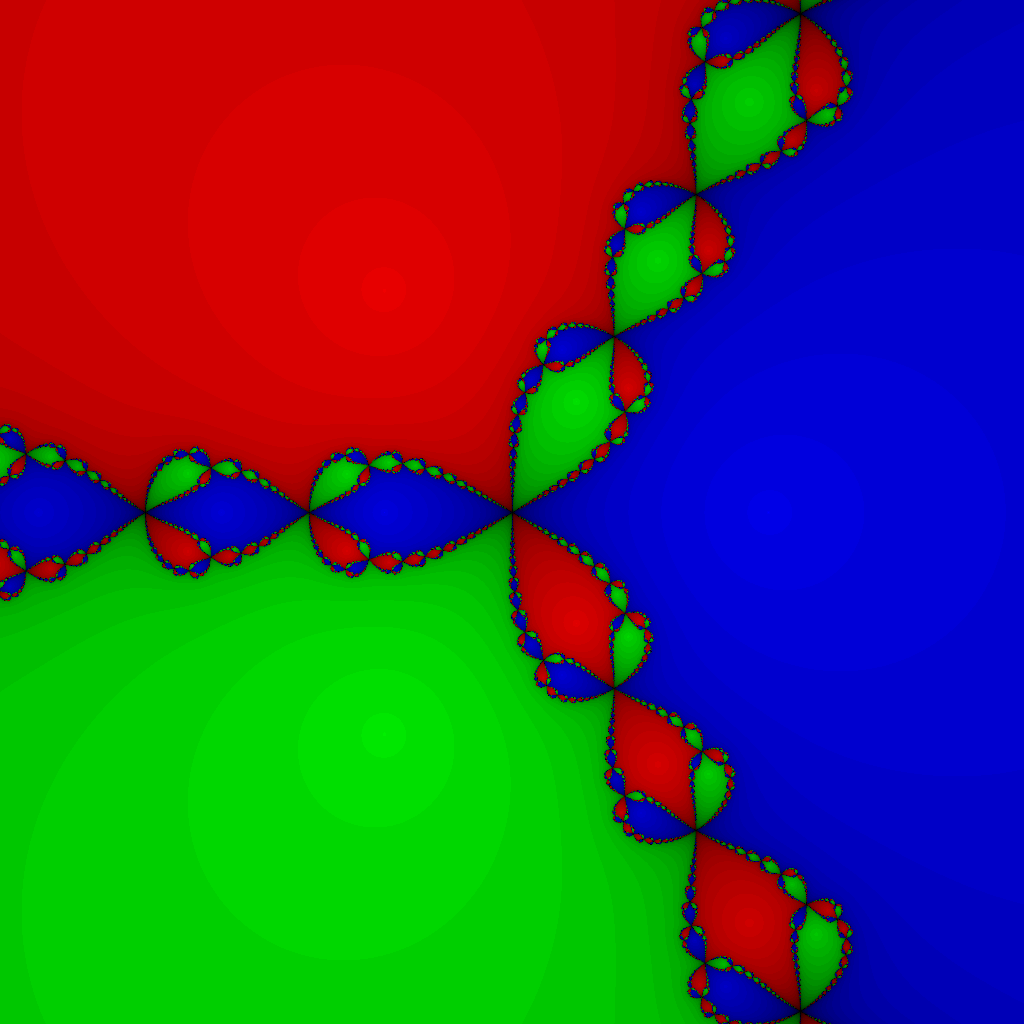
\includegraphics{newton_fractal_z_cubed_minus_one.png}
        }
        \caption{Newton Fractal for $z^{3}-1=0$}
        \label{fig:Diff_Theory_Newton_Fractal}
    \end{figure}
    The Python code used to generated this is given below.
    It can be altered to try various functions, and this
    is encouraged.
    \newpage
    \begin{lstlisting}[%
        language=python,
        basicstyle=\footnotesize\ttfamily,
        frame=single,
        gobble=16
    ]
        from PIL import Image
        import numpy as np

        # Set range for x and y axes.
        x_min, x_max = -1.0, 1.0
        y_min, y_max = -1.0, 1.0

        # Colors for the roots (Red, Green, Blue).
        colors = [(255, 0, 30), (0, 255, 30), (0, 30, 255)]

        size = 1024
        img = Image.new("RGB", (size, size), (255, 255, 255))

        # List the roots of z^3-1
        roots = [1.0+0.0j, -0.5+0.8660254037844386j, -0.5-0.8660254037844386j]
        roots = np.array(roots)
        for y in range(size):
            z_y = y * (y_max - y_min)/(size - 1) + y_min
            for x in range(size):
                z_x = x * (x_max - x_min)/(size - 1) + x_min
                z = complex(z_x, z_y)

                # Allow 40 iterations for Newton-Raphson.
                for iters in range(40):
                    # Perfrom Newton-Raphson on z^3 - 1 (Simplifying as well).
                    root = (2.0*z*z*z + 1)/(3.0*z*z)

                    # Checks for convergence
                    if abs(root - z) < 10e-10:
                        break
                    z = root

                ind = np.min((
                    np.abs(root-roots) == np.min(np.abs(root-roots))
                ).nonzero())
                col = colors[ind]
                col = [k for k in col]

                # Create a gradient in color to emphasize rate of convergence.
                col[ind] -= 10*iters
                col = tuple([k for k in col])
                img.putpixel((x, y), col)
        img.save("NewtonRoots.png", "PNG")
    \end{lstlisting}

        \chapter{Partial Differential Equations}

        \section{Green's Functions}

        \section{Kirchoff's Integral Formula}

        \section{The Wave Equation}

        \section{The Helmholtz Equation}

        \chapter{Special Functions}
    There are many special functions that arise in diffraction
    theory. These are functions that can not be written in
    closed form via a combination of rational functions,
    trigonometric functions, logarithms, or exponentials.
    Usually such functions are defined as the solution to
    a particular differential equation, such as Bessel
    functions, or as the result of integrating a non-trivial
    function, such as Fresnel Integrals. Other times functions
    are defined as the inverse of a tricky algebraic equation,
    such that the Lambert $W$ function. We'll discuss these
    three functions, numerical calculations, and their
    applications.

        \section{The Fresnel Integrals}
    The Fresnel Sine and Cosine Integrals, which are
    usually denoted $S(x)$ and $C(x)$, respectively,
    occur naturally in the study of diffraction theory.
    By examining the \textit{Fresnel Kernel},
    and using a Taylor series approximation, one
    comes across the following integral:
    \begin{equation}
        F(x)=\int_{0}^{x}\exp(it^{2})\diff{t}
    \end{equation}
    Using Euler's Theorem, we can rewrite this as:
    \begin{equation}
        F(x)=\int_{0}^{x}\cos(t^{2})\diff{t}
            +i\int_{0}^{x}\sin(t^{2})\diff{t}
    \end{equation}
    The Fresnel Cosine and Sine Integrals are defined
    as the real and
    imaginary parts of this equation, respectively.
    \begin{ldefinition}{Fresnel Integrals}
        The Fresnel Sine and Fresnel Cosine, denoted
        $S(x)$ and $C(x)$, respectively, are real valued
        functions defined by:
        \par\hfill\par
        \vspace{-1ex}
        \begin{subequations}
            \begin{minipage}{0.49\textwidth}
                \begin{equation}
                    S(x)=\int_{0}^{x}
                    \sin(t^{2})\diff{t}
                \end{equation}
            \end{minipage}
            \hfill
            \begin{minipage}{0.49\textwidth}
                \begin{equation}
                    C(x)=\int_{0}^{x}
                    \cos(t^{2})\diff{t}
                \end{equation}
            \end{minipage}
        \end{subequations}
        \par
    \end{ldefinition}
    Graph of the Fresnel Sine and Fresnel Cosine
    functions are shown in
    Fig.~\ref{fig:Diff_Theory_Graphs_of_Sinx2_and_Cosx2}.
    \begin{figure}[H]
        \captionsetup{type=figure}
        \centering
        \begin{subfigure}[b]{0.49\textwidth}
            \centering
            \resizebox{\textwidth}{!}{%
                \includegraphics{Fresnel_Cos.pdf}
            }
            \subcaption{Graphs of $\cos(x^{2})$ and $C(x)$.}
        \end{subfigure}
        %\par\hfill\par
        \begin{subfigure}[b]{0.49\textwidth}
            \centering
            \resizebox{\textwidth}{!}{%
                \includegraphics{Fresnel_Sin.pdf}
            }
            \subcaption{Graphs of $\sin(x^{2})$ and $S(x)$.}
        \end{subfigure}
        \caption[Fresnel Integrals]
            {Graphs of the Fresnel Sine and Cosine
             integrals, along with their respective derivatives.}
        \label{fig:Diff_Theory_Graphs_of_Sinx2_and_Cosx2}
    \end{figure}
    We will be interested in functions
    of the form $\exp(i\psi)$ later on. The Fresnel
    Approximation uses the Taylor expansion of $\psi$
    up to the quadratic term, and hence we will see
    something of the form $\exp(i(a+bx+cx^2))$. From
    elementary algebra we can complete the square, and
    do a change of variables to obtain
    $\exp(i(u^{2}-d^{2}))$, where $d$ is some constant.
    We are interested in the integral of this across the
    entire real line. From Euler's Formula
    (Thm.~\ref{thm:Euler_Expo_Formula}) we
    see that $\exp(ix^{2})=\cos(x^{2})+i\sin(x^{2})$.
    But $x^{2}$ grows rapidly,
    and thus $\sin(x^{2})$ and $\cos(x^{2})$ are two
    rapidly oscillating functions. The oscillation are
    so rapid that the areas cancel out, and hence
    $S(x)$ and $C(x)$ are well defined as
    $x\rightarrow\infty$. We will use Cauchy's Integral
    Theorem to evaluate the limits of these two functions.
    First, a result from Gauss.
    \begin{theorem}
        \begin{equation}
            \int_{\minus\infty}^{\infty}
                \exp(\minus{x}^{2})\diff{x}
            =\sqrt{\pi}
        \end{equation}
    \end{theorem}
    \begin{proof}
        Convergence can be shown, since for
        all $x\in\mathbb{R}$:
        \begin{equation}
            0<\exp(\minus{x}^{2})
            \leq\frac{1}{1+x^2}
        \end{equation}
        And therefore:
        \begin{equation}
            0\leq\int_{\minus\infty}^{\infty}
            \exp(\minus{x}^{2})\diff{x}\leq
            \int_{\minus\infty}^{\infty}
            \frac{1}{1+x^2}\diff{x}
            =\tan^{\minus{1}}(x)
            \Big|_{\minus\infty}^{\infty}=\pi
        \end{equation}
        Define the following:
        \begin{equation}
            \mathcal{I}=\int_{\minus\infty}^{\infty}
            \exp(\minus{x}^{2})\diff{x}
        \end{equation}
        Squaring $\mathcal{I}$, we obtain:
        \begin{subequations}
            \begin{align}
                \mathcal{I}^{2}&=
                \bigg(\int_{\minus\infty}^{\infty}
                \exp(\minus{x}^{2})\diff{x}\bigg)
                \bigg(\int_{\minus\infty}^{\infty}
                \exp(\minus{y}^{2})\diff{y}\bigg)\\
                &=\int_{\minus\infty}^{\infty}
                \int_{\minus\infty}^{\infty}
                \exp\big(\!\minus\!(x^{2}+y^{2})\big)
                    \diff{x}\diff{y}
            \end{align}
        \end{subequations}
        Switching from Cartesian to
        Polar coordinates, we have:
        \begin{equation}
            \mathcal{I}^{2}=
            \int_{0}^{2\pi}\int_{0}^{\infty}
            r\exp(\minus{r}^{2})\diff{r}\diff{\phi}
            =2\pi\int_{0}^{\infty}
            r\exp(\minus{r}^{2})\diff{r}
        \end{equation}
        This final integral can be computed from basic
        methods one would find in a Calculus textbook.
        Letting $u=r^{2}$, we have
        $\diff{u}=2r\diff{r}$,
        so the integral becomes:
        \begin{equation}
            \mathcal{I}^{2}=\pi\int_{0}^{\infty}
                \exp(\minus{u})\diff{u}
            =\pi
        \end{equation}
        Therefore $\mathcal{I}=\pm\sqrt{\pi}$.
        But $\mathcal{I}>0$, and thus
        $\mathcal{I}=\sqrt{\pi}$.
    \end{proof}
    This result has many fundamental applications in
    probability theory and in statistics, where
    it is used to define the normal distribution.
    For us, we can use this to evaluate the limits of
    $S(x)$ and $C(x)$ as $x\rightarrow\infty$.
    First note, that since $\exp(-x^{2})$ is an even
    function, the integral on $[0,\infty)$ is half of
    that of the integral on the entire real line. That is:
    \begin{equation}
        \int_{0}^{\infty}\exp(\minus{t}^{2})\diff{t}
        =\frac{\sqrt{\pi}}{2}
    \end{equation}
    We now evaluate the complex version of this.
    \begin{theorem}
        \begin{equation}
            \int_{0}^{\infty}\exp(ix^{2})\diff{x}
            =\sqrt{\frac{\pi}{8}}(1+i)
        \end{equation}
    \end{theorem}
    \begin{proof}
        For let $C_{R}$ be the closed path in the complex plane
        defined by:
        \begin{equation}
            C_{R}(t)=
            \begin{cases}
                3Rt,&0\leq{t}\leq\frac{1}{3}\\
                R\exp\big(i\frac{3\pi}{4}(t-\frac{1}{3})\big),
                &\frac{1}{3}<t<\frac{2}{3}\\
                \frac{3R}{\sqrt{2}}(1+i)(1-t),
                &\frac{2}{3}\leq{t}\leq{1}
            \end{cases}
        \end{equation}
        Then, for all $R>0$, $C_{R}$ is a Jordan Curve in the
        complex differentiable at all but three points. Thus,
        by Cauchy's Theorem, as $\exp(iz^{2})$ is an entire
        function:
        \begin{equation}
            \oint_{C_{R}}\exp(iz^{2})\diff{z}
            =0
        \end{equation}
        But then:
        \begin{equation}
            \begin{split}
                \int_{0}^{R}\exp(ix^{2})\diff{x}+
                \int_{\frac{1}{3}}^{\frac{2}{3}}&
                    \exp(iz(t)^{2})C_{R}'(t)\diff{t}\\
                &+\frac{1+i}{\sqrt{2}}\int_{R}^{0}\exp(-x^{2})\diff{x}
                =0
            \end{split}
        \end{equation}
        But by Jordan's Lemma, this second integral tends to zero as
        $R\rightarrow\infty$. Therefore:
        \begin{align}
            \int_{0}^{\infty}\exp(-ix^{2})\diff{x}
            &=-\frac{1+i}{\sqrt{2}}\int_{\infty}^{0}\exp(-x^{2})\diff{x}\\
            &=\frac{1+i}{\sqrt{2}}\int_{0}^{\infty}\exp(-x^{2})\diff{x}\\
            &=\frac{1+i}{\sqrt{2}}\frac{\sqrt{\pi}}{2}\\
            &=(1+i)\sqrt{\frac{\pi}{8}}
        \end{align}
    \end{proof}
    \begin{theorem}
        If $S$ and $C$ are the Fresnel Sine and Cosine integrals,
        respectively, then:
        \begin{align}
            \underset{x\rightarrow\infty}{\lim}S(x)
            &=\sqrt{\frac{\pi}{8}}\\
            \underset{x\rightarrow\infty}{\lim}C(x)
            &=\sqrt{\frac{\pi}{8}}
        \end{align}
    \end{theorem}
    \begin{proof}
        For:
        \begin{align}
            \underset{x\rightarrow\infty}{\lim}
                \big(C(x)+iS(x)\big)
            &=\underset{x\rightarrow\infty}{\lim}
                \int_{0}^{x}\exp(ix^{2})\diff{x}\\
            &=\sqrt{\frac{\pi}{8}}(1+i)
        \end{align}
        Comparing real and imaginary parts complex the proof.
    \end{proof}
    \begin{figure}[H]
        \centering
        \captionsetup{type=figure}
        \includegraphics{complex_plane_fresnel_integral_path.pdf}
        \caption{Jordan Curve Used to Evaluate the Fresnel Integrals.}
        \label{fig:Jordan_Curve_Fresnel_Integrals}
    \end{figure}
    \par\hfill\par
    \begin{theorem}
        If $F$ is a positive real number and
        $f:\mathbb{R}\rightarrow\mathbb{C}$ is defined by:
        \begin{equation}
            f(\rho)=
                \exp\bigg(
                    i\frac{\pi}{2}
                    \Big(\frac{\rho}{F}\Big)^{2}
                \bigg)
        \end{equation}
        Then:
        \begin{equation}
            \mathcal{F}_{\xi}(f)
            =(1+i)F\exp(\minus{2}\pi{i}F^{2}\xi^{2})
        \end{equation}
    \end{theorem}
    \begin{proof}
    For:
    \begin{align}
        \mathcal{F}_{\xi}(f)
        &=\int_{-\infty}^{\infty}
            \exp\bigg(
                i\frac{\pi}{2}
                \Big(\frac{\rho}{F}\Big)^{2}
            \bigg)
            \exp(-2\pi{i}\rho\xi)\diff{\rho}\\
        &=\int_{-\infty}^{\infty}
            \exp\bigg(
                i\frac{\pi}{2}\Big(
                    \frac{\rho}{F}
                \Big)^{2}-2\pi{i}\rho\xi
            \bigg)
            \diff{\rho}\\
        &=\int_{-\infty}^{\infty}
            \exp\Big(
                \frac{i\pi}{2F^2}
                \big[\rho^2-4F^2\rho \xi\big]
            \Big)\diff{\rho}
    \end{align}
    Completing the square, we get
    $(\rho-2F^{2}\xi)^{2}-4F^{4}\xi^{2}$.
    So, the integral becomes:
    \begin{equation}
        \begin{split}
            \int_{-\infty}^{\infty}
            \exp&\Big(
                i\frac{\pi}{2F^2}
                \big[\rho-2F^{2}\xi\big]^{2}
            \Big)
            \exp(-2\pi{i}F^{2}\xi^{2})\diff{\rho}\\
            &=\exp(-2\pi{i}F^{2}\xi^{2})
            \int_{-\infty}^{\infty}
            \exp\Big(
                i\frac{\pi}{2F^2}
                \big[\rho-2F^{2}\xi\big]^{2}
            \Big)\diff{\rho}
        \end{split}
    \end{equation}
    Let $u=\frac{\rho-2F^{2}\xi}{F}$, so then
    $F\diff{u}=\diff{\rho}$. We obtain:
    \begin{equation}
        \mathcal{F}_{\xi}(f)
        =F\exp(\minus{2}\pi{i}F^{2}\xi^{2})
            \int_{-\infty}^{\infty}
            \exp\Big(i\frac{\pi}{2}s^{2}\Big)\diff{s}
    \end{equation}
    But this integral is $1+i$, completing the proof.
    \end{proof}
    \begin{theorem}
    $\mathcal{F}(e^{-i\frac{\pi}{2}\big(\frac{\rho_0}{F}\big)^2}\big) = (1-i)Fe^{2\pi i F^2 \xi^2}$.
    \end{theorem}
    \begin{proof}
    For:
    \begin{align}
        \mathcal{F}_{\xi}(f)
        &=\int_{-\infty}^{\infty}
            \exp\bigg[
                \minus{i}\frac{\pi}{2}
                \Big(\frac{\rho}{F}\Big)^2
            \bigg]
            \exp(\minus{2}\pi{i}\rho\xi)\diff{\rho}\\
        &=\int_{-\infty}^{\infty}
            \exp\Big(
                {\!}\minus{\!}\frac{i\pi}{2F^{2}}
                \big[
                    {\rho}^{2}+4F^{2}\rho\xi
                \big]\Big)\diff{\rho}\\
        &=\int_{-\infty}^{\infty}
            \exp\Big(
                {\!}\minus{\!}\frac{i\pi}{2F^{2}}
                \big[
                    (\rho+2F^{2}\xi)^2-4F^{4}\xi^{2}
                \big]
            \Big)\diff{\rho}\\
        &=\exp(2\pi{i}F^{2}\xi^{2})\int_{-\infty}^{\infty}
            \exp\Big(
                {\!}\minus{\!}\frac{i\pi}{2F^2}
                (\rho_0+2F^2\xi)
            \Big)\diff{\rho}
    \end{align}
    Let $u = \frac{\rho_0 + 2F^2 \xi}{F}$, then
    $Fdu = d\rho_0$, so we have$Fe^{2\pi i F^2 \xi^2} \int_{-\infty}^{\infty} e^{-i\frac{\pi}{2}u^2}du$.
    Let $u = -is$, then $du = -ids$, and $u^2 = -s^2$. So
    we have $-i e^{2\pi i F^2 \xi^2}\int_{-\infty}^{\infty} e^{i\frac{\pi}{2}s^2}ds$.
    But this integral is $1+i$. So, we have
    $-iFe^{2\pi iF^2\xi^2}(1+i)=(1-i)Fe^{2\pi iF^2 \xi^2}$.
    \end{proof}
    \begin{theorem}
        If $f:\mathbb{R}\rightarrow\mathbb{R}$ and
        $g:\mathbb{R}\rightarrow{R}$ are integrable,
        and if $f*g$ is the convolution of $f$ with
        respect to $g$:
        \begin{equation}
            f*g=\int_{-\infty}^{\infty}
                f(\tau)g(\tau-t)\diff{\tau}
        \end{equation}
        Then:
        \begin{equation}
            \mathcal{F}_{\xi}\big(f*g\big)
            =\mathcal{F}_{\xi}(f)\cdot\mathcal{F}_{\xi}(g)
        \end{equation}
    \end{theorem}
    \begin{proof}
    Let $\int_{-\infty}^{\infty} |f(t)|dt = \norm{f}_{1}$ and $\int_{-\infty}^{\infty} |g(t)|dt = \norm{g}_{1}$. Then:
    \begin{align*}
        \int_{-\infty}^{\infty}\int_{-\infty}^{\infty}
            |f(\tau)g(\tau-t)|\diff{\tau}\diff{t}
        &\leq\int_{-\infty}^{\infty}
            |f(\tau)|\int_{-\infty}^{\infty}
            |g(\tau-t)|\diff{\tau}\diff{t}\\
        &=\int_{\infty}^{\infty}
            |f(x)|\norm{g}_{1}\diff{x}\\
        &=\norm{f}_{1}\norm{g}_{1}
    \end{align*}
    Thus, $h(t)=f*g$ is such that
    $\int_{-\infty}^{\infty} |h(t)|dt < \infty$.
    Let $H(\xi) = \mathcal{F}(h)$. Then:
    \begin{align}
        H(\xi)&=
            \int_{-\infty}^{\infty}
            h(t)\exp(\minus{2}\pi{i}t\xi)\diff{t}\\
        &=\int_{-\infty}^{\infty}
            \Bigg(
                \int_{-\infty}^{\infty}
                f(\tau)g(t-\tau)\diff{\tau}
            \Bigg)\exp(\minus{2}\pi{i}t\xi)\diff{t}
    \end{align}
    But:
    \begin{equation}
        |e^{-2\pi{i}t\xi}f(\tau)g(t-\tau)|
        =|f(\tau)g(t-\tau)|
    \end{equation}
    But this is simply the integrand of $h$, and $h$
    is integrable. Thus, by Fubini's Theorem we may
    swap the integrals. Let $y=t-\tau$. Then:
    \begin{subequations}
        \begin{align}
            H(\xi)&=
                \int_{-\infty}^{\infty}f(\tau)
                \int_{-\infty}^{\infty}g(t-\tau)
                e^{-2\pi{i}t\xi}\diff{t}\diff{\tau}\\
            &=\int_{-\infty}^{\infty}f(\tau)
                e^{-2\pi{i}\tau\xi}\diff{\tau}
                \int_{-\infty}^{\infty}g(y)
                e^{-2\pi{i}y\xi}dy\\
            &=\mathcal{F}(f)\cdot\mathcal{F}(g)
                \vphantom{\int_{-\infty}^{\infty}}
        \end{align}
    \end{subequations}
    Therefore, etc.
    \end{proof}
    \begin{theorem}
        If $T:\mathbb{R}\rightarrow\mathbb{C}$ is
        a Lebesgue integrable function, and if
        $\hat{T}:\mathbb{R}\rightarrow\mathbb{C}$
        is defined by:
        \begin{equation}
            \hat{T}(\rho_0)=
            \frac{1-i}{2F}\int_{\minus\infty}^{\infty}T(\rho)\exp\Big(
                i\frac{\pi}{2}\big(\frac{\rho-\rho_0}{F}\big)^{2}\Big)
            \diff{\rho}
        \end{equation}
        then:
        \begin{equation}
            T(\rho)=\frac{1+i}{2F}
                \int_{\minus\infty}^{\infty}\hat{T}(\rho_{0})\exp\Big(
                \minus{i}\frac{\pi}{2}\big(\frac{\rho-\rho_0}{F}\big)^{2}
                \Big)\diff{\rho_{0}}
        \end{equation}
    \end{theorem}
    \begin{proof}
        For by the definition of $\hat{T}$, and by the
        definition of convolution, we have:
        \begin{equation}
            \hat{T}(\rho)
            =\frac{1-i}{2F}\Big[
                T*\exp\Big(i\frac{\pi}{2}\big(\frac{\rho}{F}\big)^{2}
            \Big)\Big]
        \end{equation}
        But $T$ is a Lebesgue integrable function, and thus by
        the convolution theorem:
        \begin{subequations}
            \begin{align}
                \mathcal{F}(\hat{T})
                &=\frac{1-i}{2F}\mathcal{F}(T)\cdot
                    \mathcal{F}\Big(
                        \exp\Big[i\frac{\pi}{2}
                        \big(\frac{\rho_{0}}{F}\big)^{2}
                    \Big]\Big)\\
                &=\frac{1-i}{2F}\mathcal{F}(T)\cdot
                    (1+i)F\big(
                        \exp(\minus{2}\pi{i}F^{2}\xi^{2}
                    \big)\\
                &=\mathcal{F}(T)\exp(\minus{2}\pi{i}F^{2}\xi^{2})\\
                    \Rightarrow
                    \mathcal{F}(\hat{T})
                    \exp\big(2\pi{i}F^{2}\xi^{2}\big)
                &=\mathcal{F}(T)
            \end{align}
        \end{subequations}
        But the Fourier transform of a Gaussian is
        another Gaussian. That is:
        \begin{subequations}
            \begin{align}
                \exp\big(2\pi{i}F^{2}\xi^{2}\big)
                &=\frac{1}{(1-i)F}\mathcal{F}\Big(
                    \exp\Big[\minus{i}\frac{\pi}{2}
                    \big(\frac{\rho_{0}}{F}\big)^{2}\Big]\Big)\\
                &=\frac{1+i}{2F}\mathcal{F}\Big(
                    \exp\Big[\minus{i}\frac{\pi}{2}
                        \big(\frac{\rho_0}{F}\big)^{2}
                    \Big]\Big)
            \end{align}
        \end{subequations}
        Therefore:
        \begin{subequations}
            \begin{align}
                \mathcal{F}(T)
                &=\frac{1+i}{2F}\mathcal{F}(\hat{T})
                    \cdot\mathcal{F}
                    \big(e^{-i\frac{\pi}{2}
                    \big(\frac{\rho_0}{F}\big)^2}\big)\\
                &=\frac{1+i}{2F}\mathcal{F}
                    (\hat{T}*e^{-i\frac{\pi}{2}
                    \big(\frac{\rho_0}{F}\big)^2})\\
            &=\mathcal{F}\bigg(\frac{1+i}{2F}
                \int_{\minus\infty}^{\infty}\hat{T}(\rho_{0})
                \exp\Big[\minus{i}\frac{\pi}{2}\big(
                    \frac{\rho-\rho_{0}}{F}\big)^{2}\Big]
                \diff{\rho_{0}}\bigg)
            \end{align}
        \end{subequations}
        Therefore, by the uniqueness of the Fourier Transform:
        \begin{equation}
            T(\rho)=\frac{1+i}{2F}\int_{-\infty}^{\infty}
                \hat{T}(\rho_{0})\exp\Big[
                    \!\minus\!\frac{i\pi}{2}
                    \big(\frac{\rho-\rho_{0}}{F}\big)^{2}
                \Big]\diff{\rho_{0}}
        \end{equation}
        Therefore, etc.
    \end{proof}
    \begin{theorem}
            If $T,\psi\in{L}^{2}(\mathbb{R})$, and if
            $\hat{T}:\mathbb{R}\rightarrow\mathbb{C}$
            is defined by:
            \begin{equation}
            T(\rho_{0})=\int_{\minus\infty}^{\infty}
                T(\rho)\exp\big(i\psi(\rho_{0}-\rho)\big)
                \diff{\rho_{0}}
            \end{equation}
            then:
            \begin{equation}
                T(\rho)=\mathcal{F}^{\minus{1}}_{\rho}\Big(
                    \frac{\mathcal{F}(\hat{T})}
                        {\mathcal{F}\big(\exp(i\psi)\big)}
                    \Big)
            \end{equation}
    \end{theorem}
    \begin{proof}
        For $\hat{T}(\rho_{0})=T*\exp(i\psi)$. But then:
        \begin{equation}
            \mathcal{F}_{\xi}(\hat{T})
            =\mathcal{F}_{\xi}\big(T*\exp(i\psi)\big)
            =\mathcal{F}_{\xi}\big(T\big)\cdot
            \mathcal{F}\big(\exp(i\psi)\big)
        \end{equation}
        So then:
        \begin{equation}
            \mathcal{F}_{\xi}(T)
            =\frac{\mathcal{F}(\hat{T})}
                {\mathcal{F}\big(\exp(i\psi)\big)}
        \end{equation}
        From the uniqueness of Fourier transforms, we
        obtain the result.
    \end{proof}

        \section{Bessel Functions}

        \section{Lambert $W$ Function}

        \section{Legendre Polynomials}

    \part{Theory}
        \chapter{Diffraction Theory}

        \section{Maxwell's Equations}
    At the heart of electromagnetism are Maxwell's equations.
    They are:
    \par
    \begin{subequations}
        \begin{minipage}[b]{0.49\textwidth}
            \centering
            \begin{align}
                \mathrm{curl}(\mathbf{E})
                    &=\minus\frac{\partial\mathbf{B}}{\partial{t}}\\
                \mathrm{div}(\mathbf{E})
                    &=\frac{\rho}{\epsilon_{0}}
            \end{align}
        \end{minipage}
        \hfill
        \begin{minipage}[b]{0.49\textwidth}
            \centering
            \begin{align}
                \mathrm{curl}(\mathbf{B})
                    &=\mu_{0}\mathbf{J}+\mu_{0}\epsilon_{0}
                      \frac{\partial\mathbf{E}}{\partial{t}}\\
                \mathrm{div}(\mathbf{B})&=0
            \end{align}
        \end{minipage}
    \end{subequations}
    \par
    With this, we will derive the Fresnel-Huygens principle.
        \section{Fresnel-Fraunhofer Theory}
        \section{Fresnel's Approximation}
        \section{Fresnel Inversion}
    \subsection{Diffraction Through a Square Well}
        \label{Subsec:Cassini_Math_Diffraction_Through_a_Square_well}
        We wish to solve for $\hat{T}(\rho_{0})$. We have that:
        \begin{equation}
            \hat{T}(\rho_{0})
            =\frac{1-i}{2F}
                \int_{-\infty}^{\infty}T(\rho)
                \exp\Big(i\frac{\pi}{2}
                    \big(\frac{\rho-\rho_{0}}{F}\big)^{2}\Big)
                \diff{\rho}
        \end{equation}
        For the square well of height $M$
        starting at $a$ and ending at $b$:
        \begin{equation}
            T(\rho)=
            \begin{cases}
                0,&\rho<a\\
                M,&a\leq\rho\leq{b}\\
                0,&b<\rho
            \end{cases}
        \end{equation}
        Let $H_{M}(\rho_0,F;a,b)$ denote the solution.
        So, we have:
        \begin{subequations}
            \begin{align}
                H_{M}(\rho_0,F;a,b)
                &=\frac{1-i}{2F}\int_{a}^{b}M
                    \exp\Big(
                        \frac{i\pi}{2}
                        \big(\frac{\rho-\rho_{0}}{F}\big)^{2}
                    \Big)\diff{\rho}\\
                &=\frac{M}{F}\frac{1-i}{2}
                    \int_{a}^{b}
                    \exp\Big(
                        \frac{i\pi}{2}
                        \big(\frac{\rho-\rho_{0}}{F}\big)^{2}
                    \Big)\diff{\rho}
            \end{align}
        \end{subequations}
        Now from Euler's formula,
        $\exp(i\theta)=\cos(\theta)+i\sin(\theta).$
        Using this we obtain:
        \begin{equation}
            \exp\Big(
                \frac{i\pi}{2}
                \big(\frac{\rho-\rho_{0}}{F}\big)^{2}
            \Big)
            =\cos\Big(
                \frac{\pi}{2}
                \big(\frac{\rho-\rho_{0}}{F}\big)^{2}
            \Big)+
            i\sin\Big(
                \frac{\pi}{2}
                \big(\frac{\rho-\rho_{0}}{F}\big)^{2}
            \Big)
        \end{equation}
        Recall the Fresnel Cosine Integral and
        Sine Integrals $\big(C(x),S(x)\big)$ are defined as:
        \par
        \begin{subequations}
            \begin{minipage}[b]{0.49\textwidth}
                \begin{equation}
                    S(x)=\int_{0}^{x}\sin(t^{2})\diff{t}
                \end{equation}
            \end{minipage}
            \hfill
            \begin{minipage}[b]{0.49\textwidth}
                \begin{equation}
                    C(x)=\int_{0}^{x}\cos(t^{2})\diff{t}
                \end{equation}
            \end{minipage}
        \end{subequations}
        Letting $u=\sqrt{\frac{\pi}{2}}x$, we obtain:
        \begin{subequations}
            \begin{align}
                \int_{a}^{b}\sin\Big(\frac{\pi}{2}x^{2}\Big)\diff{x}
                &=\int_{0}^{b}\sin\Big(\frac{\pi}{2}x^{2}\Big)\diff{x}-
                    \int_{0}^{a}\sin\Big(\frac{\pi}{2}x^{2}\Big)\diff{x}\\
                &=\sqrt{\frac{2}{\pi}}\Bigg[
                    \int_{0}^{\sqrt{\frac{\pi}{2}}b}\sin(u^{2})\diff{u}-
                    \int_{0}^{\sqrt{\frac{\pi}{2}}a}\sin(u^{2})\diff{u}
                \Bigg]\\
                &=\sqrt{\frac{2}{\pi}}\Big[
                    S\Big(\sqrt{\frac{\pi}{2}}b\Big)-
                    S\Big(\sqrt{\frac{\pi}{2}}a\Big)
                \Big]\\
                    \int_{a}^{b}\cos\Big(\frac{\pi}{2}x^{2}\Big)\diff{x}
                &=\int_{0}^{b}\cos\Big(\frac{\pi}{2}x^{2}\Big)\diff{x}-
                    \int_{0}^{a}\cos\Big(\frac{\pi}{2}x^{2}\Big)\diff{x}\\
                &=C(b)-C(a)
            \end{align}
        \end{subequations}
        We can now compute
        $H_{M}(\rho_0,F;a,b)$.
        Let $x=\frac{\rho-\rho_0}{F}$. Then $dx = \frac{d\rho}{F}$.
        We have:
        \begin{align*}
            H_{M}(\rho_0,F;a,b)
            &=\frac{M}{F}\frac{1-i}{2}
                \int_{a}^{b}
                \exp\Big(i\frac{\pi}{2}
                \big(\frac{\rho-\rho_0}{F}\big)^{2}\Big)
            \diff{\rho}\\
            &=\frac{M}{F}\frac{1-i}{2}
                \bigg[\int_{a}^{b}
                \cos\Big(\frac{\pi}{2}
                \big(\frac{\rho-\rho_0}{F}\big)^{2}\Big)
            \diff{\rho}+
            i\int_{a}^{b}
                \sin\Big(\frac{\pi}{2}
                \big(\frac{\rho-\rho_0}{F}\big)^{2}\Big)
                \diff{\rho}\bigg]\\
            &=M\frac{1-i}{2}\bigg[
                \int_{\frac{a-\rho_0}{F}}^{\frac{b-\rho_0}{F}}
                \cos\Big(\frac{\pi}{2}x^{2}\Big)\diff{x}+
            i\int_{\frac{a-\rho_0}{F}}^{\frac{b-\rho_0}{F}}
                \sin\Big(\frac{\pi}{2}x^{2}\Big)\diff{x}
            \bigg]\\
            &=M\frac{1-i}{2}
                \bigg[\bigg(C\Big(\frac{b-\rho_{0}}{F}\Big)-
                    C\Big(\frac{a-\rho_0}{F}\Big)\bigg)
                +i\bigg(S\Big(\frac{b-\rho_0}{F}\Big)-
                    S\Big(\frac{a-\rho_0}{F}\Big)\bigg)\bigg]
        \end{align*}
    \subsection{Diffraction Through an Inverted Square Well}
        This time we have:
        \begin{equation*}
            T(\rho)=
            \begin{cases}
                M,&\rho<a\\
                0,&a\leq\rho\leq{b}\\
                M,&b<\rho
            \end{cases}
        \end{equation*}
        So $T(\rho) = M - T_{Sq}(\rho)$,
        where $T_{Sq}(\rho)$ is the impulse from the standard
        square well (See
        \ref{Subsec:Cassini_Math_Diffraction_Through_a_Square_well}).
        So we wish to solve:
        \begin{equation*}
            \hat{T}(\rho_{0})=
            \frac{1-i}{2F}\int_{-\infty}^{\infty}
            \big(M-T_{Sq}(\rho)\big)
            \exp(i\frac{\pi}{2}\Big(\frac{\rho-\rho_{0}}{F}\Big)^{2})
            \diff{\rho}
        \end{equation*}
            Simplifying, we have:
            \begin{align*}
                \hat{T}(\rho_{0})
                &=\frac{1-i}{2F}\int_{-\infty}^{\infty}
                \big(M-T(\rho)\big)
                \exp\Big(i\frac{\pi}{2}
                    \big(\frac{\rho-\rho_0}{F}\big)^{2}\Big)
                \diff{\rho}\\
                &=\frac{M}{F}\frac{1-i}{2}
                \bigg(\int_{-\infty}^{\infty}
                \exp\Big(i\frac{\pi}{2}
                    \big(\frac{\rho-\rho_0}{F}\big)^2\Big)
                \diff{\rho}-
                \int_{a}^{b}
                \exp\Big(i\frac{\pi}{2}
                    \big(\frac{\rho-\rho_0}{F}\big)^2\Big)
                \diff{\rho}\Bigg)\\
            \end{align*}
            But from the previous derivation:
            \begin{equation*}
                \int_{a}^{b}
                \exp\Big(i\frac{\pi}{2}
                    \big(\frac{\rho-\rho_0}{F}\big)^{2}\Big)
                \diff{\rho}
                =F\bigg(C\Big(\frac{b-\rho_0}{F}\Big)-
                C\Big(\frac{a-\rho_0}{F}\Big)\bigg)+
                i\bigg(S\Big(\frac{b-\rho_0}{F}\Big)-
                S\Big(\frac{a-\rho_0}{F}\Big)\bigg)
            \end{equation*}
            And:
            \begin{equation*}
                \int_{-\infty}^{\infty}
                \exp\Big(i\frac{\pi}{2}
                    \big(\frac{\rho-\rho_0}{F}\big)^{2}\Big)
                \diff{\rho}
                =\underset{a\rightarrow \infty}{\lim}
                \int_{-a}^{a}
                \exp\Big(i\frac{\pi}{2}
                    \big(\frac{\rho-\rho_0}{F}\big)^{2}\Big)
                \diff{\rho}
                =F(1+i)
            \end{equation*}
            Piecing this together, and using the notation from before,
            we have:
            \begin{equation*}
            \hat{T}(\rho_0)=M-H_{M}(\rho_0,F;a,b)
            \end{equation*}

        \chapter{Geometry}
    \section{Titan Geometry}
        \begin{figure}[H]
        	\centering
        	\captionsetup{type=figure}
        	\begin{subfigure}[b]{0.49\textwidth}
        	    \centering
        	    \captionsetup{type=figure}
        	    \resizebox{\textwidth}{!}{%
                  \includegraphics{titan_occultation_geometry.pdf}
              }
            	\subcaption{Geometry of an Occultation of Titan}
        	    \label{fig:math_titan_geom_vec}
            \end{subfigure}
            \begin{subfigure}[b]{0.49\textwidth}
                \centering
                \captionsetup{type=figure}
                \resizebox{\textwidth}{!}{%
                    \includegraphics{titan_bending_angle_geometry.pdf}
                }
                \subcaption{Geometry of the Bending Angle}
                \label{fig:math_geo_bending_angle}
            \end{subfigure}
            \caption{Various Geometries for Titan}
        \end{figure}
        The following definitions are used:
        \begin{enumerate}
            \item $O$ is the center of Titan.
            \item $E$ is the Earth.
            \item $C$ is the Cassini spacecraft.
            \item $\mathbf{r}_{E}=\overrightarrow{OE}$
            \item $\mathbf{v}_{E}=\dot{\mathbf{r}}_{E}$
            \item $\mathbf{r}_{S}=\overrightarrow{OC}$
            \item $\mathbf{v}_{S}=\dot{\mathbf{r}}_{S}$
            \item $\mathbf{p}_{in}$ is the projection of
                  $O$ onto $\overline{AC}$
            \item $\mathbf{p}_{out}$ is the projection
                  of $O$ onto $\overline{EA}$
            \item $\alpha$ is the bending angle
                  ($\pi-\angle EAC$)
            \item $\hat{\mathbf{n}}_{in}$ is the
                  direction of the emission.
            \item $\hat{\mathbf{n}}_{out}$ is the
                  direction of the reception.
            \item The ray plane lies in the plane $OEC$
            \item $\phi=\angle{AOC}$
            \item $\theta=\angle{ACO}$
            \item $\beta=\angle{OAC}$
            \item $A$ is the intersection of the lines
                  starting at $C$ and $E$, parallel to
                  $\hat{\mathbf{n}}_{in}$ and
                  $\hat{\mathbf{n}}_{out}$, respectively.
        \end{enumerate}

        % Replace the 6pt vspace removed to below the list.
        \vspace{6pt}
        Where $\dot{\mathbf{r}}$ denotes the time derivative
        of $\mathbf{r}$. The following assumptions are made:
        \begin{enumerate}
            \item $\angle{OAE}=\angle{OAC}$
            \item $A$ lies in the plane $OEC$
        \end{enumerate}
        \begin{theorem}
            \label{theorem:ray_plane_perp_to_r_e_cross_r_s}
            The ray plane is perpendicular to
            $\hat{\mathbf{z}}%
             =\frac{\mathbf{r}_{S}\times
             \mathbf{r}_{E}}{\norm{\mathbf{r}_{S}\times
             \mathbf{r}_{E}}}$
        \end{theorem}
        \begin{proof}
            As the ray plane is the plane $OEC$,
            $\mathbf{r}_{S}$ and $\mathbf{r}_{E}$ lie parallel
            to this plane. Moreover, during an occultation,
            $\mathbf{r}_{S}$ and $\mathbf{r}_{E}$ are not
            parallel and therefore $OEC$ is uniquely determined
            by $\mathbf{r}_{E}$, $\mathbf{r}_{S}$, and the point
            $O$. But
            $\hat{\mathbf{z}}%
             =\frac{\mathbf{r}_{S}\times
             \mathbf{r}_{E}}{\norm{\mathbf{r}_{S}\times
             \mathbf{r}_{E}}}$
            is perpendicular to both $\mathbf{r}_{E}$ and
            $\mathbf{r}_{S}$. Therefore $\hat{\mathbf{z}}$ is
            perpendicular to the ray plane.
        \end{proof}
        \begin{theorem}
            \label{theorem:r_e_dot_p_out_equal_p_out_square}
            $\mathbf{r}_{E}\cdot\mathbf{p}_{out}%
             =\norm{\mathbf{p}_{out}}^{2}$
        \end{theorem}
        \begin{proof}
            $\mathbf{p}_{out}$ is the projection of the $O$
            onto $\overline{EA}$. But $\overline{EA}$ lies
            parallel to $\hat{\mathbf{n}}_{out}$, and
            therefore $\mathbf{p}_{out}$ and
            $\hat{\mathbf{n}}_{out}$ are orthogonal,
            and thus
            $\mathbf{p}_{out}\cdot\hat{\mathbf{n}}_{out}=0$.
            Moreoever,
            $\mathbf{r}_{E}%
             =\mathbf{p}_{out}+(\mathbf{r}_{E}\cdot
             \hat{\mathbf{n}}_{out}) \hat{\mathbf{n}}_{out}$.
            But then:
            \begin{align*}
                \mathbf{p}_{out}\cdot \mathbf{r}_{E}
                &=\mathbf{p}_{out}\cdot\big(
                    \mathbf{p}_{out}
                    +(\mathbf{r}_{E}\cdot
                    \hat{\mathbf{n}}_{out})
                    \hat{\mathbf{n}}_{out}
                \big)\\
                \Rightarrow\mathbf{p}_{out}\cdot \mathbf{r}_{E}
                &=\mathbf{p}_{out}\cdot\mathbf{p}_{out}
                 +(\mathbf{r}_{E}\cdot\hat{\mathbf{n}}_{out})
                  \mathbf{p}_{out}\cdot \hat{\mathbf{n}}_{out}\\
                \Rightarrow\mathbf{p}_{out}\cdot\mathbf{r}_{E}
                &=\mathbf{p}_{out}\cdot\mathbf{p}_{out}
            \end{align*}
            Therefore
            $\mathbf{p}_{out}\cdot\mathbf{r}_{E}%
             =\norm{\mathbf{p}_{out}}^{2}$
        \end{proof}
        \begin{theorem}
            $\alpha%
             =\cos^{-1}(\hat{\mathbf{n}}_{in}
              \cdot\hat{\mathbf{n}}_{out})$
        \end{theorem}
        \begin{proof}
            By definition,
            $\alpha=\pi-\angle{EAC}$.
            But $\hat{\mathbf{n}}_{out}$ lies parallel to
            $\overrightarrow{AE}$, and $-\hat{\mathbf{n}}_{in}$
            lies parallel to $\overrightarrow{AC}$. Therefore:
            \begin{equation*}
                -\hat{\mathbf{n}}_{out}\cdot
                 \hat{\mathbf{n}}_{in}
                =\hat{\mathbf{n}}_{out}\cdot
                 (-\hat{\mathbf{n}}_{in})
                =\norm{\hat{\mathbf{n}}_{out}}
                 \norm{-\hat{\mathbf{n}}_{in}}\cos(\angle{EAC})
            \end{equation*}
            But $\hat{\mathbf{n}}_{in}$ and
            $\hat{\mathbf{n}}_{out}$ are unit vectors,
            and therefore
            $\norm{\hat{\mathbf{n}}_{out}}%
             =\norm{-\hat{\mathbf{n}}_{in}}=1$.
            Therefore:
            \begin{equation*}
                \angle EAC
                =\cos^{-1}(
                    -\hat{\mathbf{n}}_{out}\cdot
                    \hat{\mathbf{n}}_{in}
                )
            \end{equation*}
            But $\alpha=\pi-\angle{EAC}$,
            and $\cos^{-1}(-x)=\pi-\cos^{-1}(x)$.
            Therefore:
            \begin{equation*}
                \alpha=\pi-\angle{EAC}
                =\pi-\big(
                    \pi-\cos^{-1}(\hat{\mathbf{n}}_{out}\cdot
                    \hat{\mathbf{n}}_{in})
                \big)
                =\cos^{-1}(\hat{\mathbf{n}}_{out}\cdot
                 \hat{\mathbf{n}}_{in})
            \end{equation*}
        \end{proof}
        \begin{theorem}
            $\theta%
             =\cos^{-1}\big(%
                  \frac{(-\mathbf{r}_{S})\cdot%
                  \hat{\mathbf{n}}_{in}}{\norm{\mathbf{r}_{S}}}%
              \big)$
        \end{theorem}
        \begin{proof}
            For $\theta=\angle OCA$.
            But $\hat{\mathbf{n}}_{in}$ is parallel with
            $\overrightarrow{CA}$, and $(-\mathbf{r}_{S})$
            is parallel with $\overrightarrow{CO}$.
            Therefore:
            \begin{align*}
                (-\mathbf{r}_{S})\cdot\hat{\mathbf{n}}_{in}
                &=\norm{(-\mathbf{r}_{S})}
                  \norm{\hat{\mathbf{n}}_{in}}\cos(\theta)\\
                \Rightarrow\theta
                &=\cos^{-1}\bigg(
                    \frac{%
                        (-\mathbf{r}_{S})\cdot
                        \hat{\mathbf{n}}_{in}
                    }{\norm{\mathbf{r}_{S}}}
                \bigg)
            \end{align*}
        \end{proof}
        \begin{theorem}
            \begin{equation*}
                \beta=\pi-\frac{1}{2}\cos^{-1}
                \Big(\frac{\mathbf{r}_{s}
                     \cdot\mathbf{r}_{E}}
                     {\norm{\mathbf{r}_{s}}
                     \norm{\mathbf{r}_{E}}}\Big)
                -\frac{1}{2}\cos^{-1}
                \Big(\frac{\mathbf{r}_{E}\cdot
                           \hat{\mathbf{n}}_{out}}
                          {\norm{\mathbf{r}_{E}}}\Big)
                -\frac{1}{2}\cos^{-1}
                \Big(\frac{(-\mathbf{r}_{s})\cdot
                           \hat{\mathbf{n}}_{in}}
                          {\norm{\mathbf{r}_{s}}}\Big)
            \end{equation*}
        \end{theorem}
        \begin{proof}
            The sum of the angles in $OEAC$ is $2\pi$.
            But
            $\angle{OAE}=\angle{OAC}=\phi$, and therefore:
            \begin{align*}
                2\beta&=\angle{EAC}\\
                \Rightarrow
                2\pi
                &=2\beta+\angle{AEO}
                 +\angle{EOC}+\angle{OCA}\\
                \Rightarrow\beta
                &=\pi-\frac{\angle{AEO}}{2}
                 -\frac{\angle EOC}{2}-\frac{\angle OCA}{2}
            \end{align*}
            But:
            \begin{align*}
                (-\hat{\mathbf{n}}_{out})\cdot
                (-\hat{\mathbf{r}}_{E})
                &=\norm{\mathbf{r}_{E}}\cos(\angle AEO)\\
                \Rightarrow\angle{AEO}
                &=\cos^{-1}\bigg(
                    \frac{
                        \hat{\mathbf{n}}_{out}\cdot
                        \mathbf{r}_{E}
                    }{\norm{\mathbf{r}_{E}}}
                \bigg)
            \end{align*}
            Also:
            \begin{align*}
                \mathbf{r}_{E}\cdot\mathbf{r}_{S}
                &=\norm{\mathbf{r}_{E}}
                  \norm{\mathbf{r}_{S}}\cos(\angle EOC)\\
                \Rightarrow\angle{EOC}
                &=\cos^{-1}
                  \bigg(
                      \frac{
                          \mathbf{r}_{E}\cdot
                          \mathbf{r}_{S}
                      }{
                          \norm{\mathbf{r}_{E}}
                          \norm{\mathbf{r}_{S}}
                      }
                  \bigg)
            \end{align*}
            But
            $\angle{OCA}%
             =\theta%
             =\cos^{-1}%
              \big(\frac{%
                       (-\mathbf{r}_{S})\cdot%
                       \hat{\mathbf{n}}_{in}%
                   }{\norm{\mathbf{r}_{S}}}%
              \big)$.
            Therefore:
            \begin{equation*}
                \beta=\pi-\frac{1}{2}\cos^{-1}
                    \bigg(
                        \frac{
                            \mathbf{r}_{s}\cdot
                            \mathbf{r}_{E}
                        }{
                            \norm{\mathbf{r}_{s}}
                            \norm{\mathbf{r}_{E}}
                        }
                    \bigg)
                    -\frac{1}{2}\cos^{-1}
                    \bigg(
                        \frac{
                            \mathbf{r}_{E}\cdot
                            \hat{\mathbf{n}}_{out}
                        }{
                            \norm{\mathbf{r}_{E}}
                        }
                    \bigg)
                    -\frac{1}{2}\cos^{-1}
                    \bigg(
                        \frac{
                            (-\mathbf{r}_{s})\cdot
                            \hat{\mathbf{n}}_{in}
                        }{
                            \norm{\mathbf{r}_{s}}
                        }
                    \bigg)
            \end{equation*}
        \end{proof}
        \begin{theorem}
            $\alpha=\pi-2\beta$
        \end{theorem}
        \begin{proof}
            $\alpha$ and $\angle EAC$ are supplementary to
            the ray $\overrightarrow{CA}$, and therefore
            $\alpha+\angle EAC=\pi$.
            But $\angle{EAC}=\angle{EAC}+\angle{OAC}=2\beta$.
            Therefore $\alpha+2\beta=\pi$.
            Thus, $\alpha=\pi-2\beta$.
        \end{proof}
        \begin{theorem}
            $\theta=\frac{\pi}{2}+\frac{\alpha}{2}-\phi$
        \end{theorem}
        \begin{proof}
            As the angles of a triangle sum to $\pi$,
            $\theta+\beta+\phi=\pi$. But
            $\alpha=\pi-2\beta\Rightarrow\beta%
             =\frac{\pi}{2}-\frac{\alpha}{2}$.
            So we have:
            \begin{align*}
                \theta+\phi+\beta
                &=\pi\\
                \Rightarrow
                \theta+\phi+\frac{\pi}{2}-\frac{\alpha}{2}
                &=\pi\\
                \Rightarrow\theta
                &=\frac{\pi}{2}+\frac{\alpha}{2}-\phi
            \end{align*}
        \end{proof}
        \begin{theorem}
            \begin{equation*}
                \phi=\frac{1}{2}\cos^{-1}
                    \Big(\frac{\mathbf{r}_{s}\cdot
                               \mathbf{r}_{E}}
                              {\norm{\mathbf{r}_{s}}
                               \norm{\mathbf{r}_{E}}}\Big)
                +\frac{1}{2}\cos^{-1}
                \Big(\frac{\mathbf{r}_{E}\cdot
                           \hat{\mathbf{n}}_{out}}
                          {\norm{\mathbf{r}_{E}}}\Big)
                -\frac{1}{2}\cos^{-1}
                \Big(\frac{(-\mathbf{r}_{s})\cdot
                           \hat{\mathbf{n}}_{in}}
                          {\norm{\mathbf{r}_{s}}}\Big)
            \end{equation*}
        \end{theorem}
        \begin{proof}
            For:
            \begin{align*}
                \pi&=\beta+\theta+\phi\\
                \theta
                &=\cos^{-1}
                    \bigg(
                        \frac{
                            (-\mathbf{r}_{S})\cdot
                            \hat{\mathbf{n}}_{in}
                        }{\norm{\mathbf{r}_{S}}}
                    \bigg)\\
                \beta&= \pi-\frac{1}{2}\cos^{-1}
                    \bigg(
                        \frac{
                            \mathbf{r}_{s}\cdot
                            \mathbf{r}_{E}
                        }{
                            \norm{\mathbf{r}_{s}}
                            \norm{\mathbf{r}_{E}}
                        }
                    \bigg)
                    -\frac{1}{2}\cos^{-1}
                        \bigg(
                            \frac{
                                \mathbf{r}_{E}\cdot
                                \hat{\mathbf{n}}_{out}
                            }{\norm{\mathbf{r}_{E}}}
                        \bigg)
                        -\frac{1}{2}\cos^{-1}
                            \bigg(
                                \frac{
                                    (-\mathbf{r}_{s})\cdot
                                    \hat{\mathbf{n}}_{in}
                                }{\norm{\mathbf{r}_{s}}}
                            \bigg)\\
                \Rightarrow\phi
                &=\frac{1}{2}\cos^{-1}
                    \bigg(
                        \frac{
                            \mathbf{r}_{s}\cdot
                            \mathbf{r}_{E}
                        }{
                            \norm{\mathbf{r}_{s}}
                            \norm{\mathbf{r}_{E}}
                        }
                    \bigg)
                 +\frac{1}{2}\cos^{-1}
                     \bigg(
                         \frac{
                             \mathbf{r}_{E}\cdot
                             \hat{\mathbf{n}}_{out}
                         }{
                             \norm{\mathbf{r}_{E}}
                         }
                     \bigg)
                 -\frac{1}{2}\cos^{-1}
                     \bigg(
                         \frac{
                             (-\mathbf{r}_{s})\cdot
                             \hat{\mathbf{n}}_{in}
                         }{
                             \norm{\mathbf{r}_{s}}
                         }
                     \bigg)
            \end{align*}
        \end{proof}
        \begin{theorem}
            \label{%
                theorem:impact_parameter_p_%
                closed_form_solution
            }
            $p=\norm{\mathbf{p}_{in}}%
              =\norm{\mathbf{r}_{S}}%
               \cos(\phi-\frac{\alpha}{2})$
        \end{theorem}
        \begin{proof}
            As $P$ is the orthogonal projection of $O$
            onto $\overline{CA}$,
            $\angle{OPC}=\frac{\pi}{2}$. But then:
            \begin{equation*}
                |\overline{OP}|
                =|\overline{OC}|\sin(\angle{OCP})
            \end{equation*}
            But $|\overline{OP}|=\norm{\mathbf{p}_{in}}$,
            $|\overline{OC}|=\norm{\mathbf{r}_{S}}$,
            and $\angle{OCP}=\theta$. Therefore:
            \begin{equation*}
                \norm{\mathbf{p}_{in}}
                =\norm{\mathbf{r}_{S}}\sin(\theta)
            \end{equation*}
            But $\theta=\frac{\pi}{2}+\frac{\alpha}{2}-\phi$,
            and $\sin(\frac{\pi}{2}+x)=\cos(x)$. Therefore:
            \begin{equation*}
                \norm{\mathbf{p}_{in}}
                =\norm{\mathbf{r}_{S}}\cos
                    \big(\frac{\alpha}{2}-\phi\big)
            \end{equation*}
        \end{proof}
        \begin{theorem}
            $\norm{\mathbf{p}_{in}}%
             =|\overline{OA}|\sin(\beta)$
        \end{theorem}
        \begin{proof}
            For $\overline{OP}$ is perpendicular to
            $\overline{CA}$, and therefore $\Delta OPA$
            is a right-angled triangle, and $\overline{OA}$
            is the hypotenuse. Moreoever
            $\angle{PAO}=\beta$. But then:
            \begin{align*}
                |\overline{OP}|
                &=|\overline{OA}|\sin(\angle PAO)\\
                \Rightarrow|OP|
                &=|\overline{OA}|\sin(\beta)
            \end{align*}
            But $\norm{\mathbf{p}_{in}}=|\overline{OP}|$, and
            thus $\norm{\mathbf{p}_{in}}=|OA|\sin(\beta)$
        \end{proof}
        \begin{theorem}
            \label{theorem:p_out_equals_p_in}
            $\norm{\mathbf{p}_{in}}=\norm{\mathbf{p}_{out}}$
        \end{theorem}
        \begin{proof}
            For $\angle OAE=\angle{OAC}=\beta$, and thus:
            \begin{equation*}
                \norm{\mathbf{p}}_{out}
                =|\overline{OA}|\sin(\angle OAE)
                =|\overline{OA}|\sin(\beta)
                =\norm{\mathbf{p}}_{in}
            \end{equation*}
        \end{proof}
    \section{Ring Geometry}
        \begin{theorem}
            \label{theorem:ring_occ_geom_x_y_z_orthonormal_basis}
            If $\hat{\mathbf{u}}$ and $\hat{\mathbf{z}}$ are unit
            vectors and
            $\hat{\mathbf{u}}\times%
             \hat{\mathbf{z}}\ne\mathbf{0}$,
            then:
            \begin{equation}
                \label{eqn:Cassini_Math_Saturn_Basis}
                \{\hat{\mathbf{x}},\hat{\mathbf{y}},
                \hat{\mathbf{z}}\}
                =\Big\{\big(
                    \frac{\hat{\mathbf{u}}\times\hat{\mathbf{z}}}
                         {\norm{\hat{\mathbf{u}}\times
                          \hat{\mathbf{z}}}}
                \big)\times\hat{\mathbf{z}},
                \frac{\hat{\mathbf{u}}\times\hat{\mathbf{z}}}
                     {\norm{\hat{\mathbf{u}}\times
                      \hat{\mathbf{z}}}},
                \hat{\mathbf{z}}\Big\}
            \end{equation}
            is an orthonormal basis of $\mathbb{R}^{3}$.
        \end{theorem}
        \begin{proof}
            Since $\hat{\mathbf{u}}\times\hat{\mathbf{z}}$ is a
            non-zero vector,
            $\norm{\mathbf{u}\times\mathbf{z}}\ne{0}$. Thus, let
            $\hat{\mathbf{y}}%
             =\frac{\hat{\mathbf{u}}\times\hat{\mathbf{z}}}%
                   {\norm{\hat{\mathbf{u}}\times\hat{\mathbf{z}}}}$
            and let
            $\hat{\mathbf{x}}%
             =\hat{\mathbf{y}}\times\hat{\mathbf{z}}$.
            Then $\hat{\mathbf{y}}\cdot\hat{\mathbf{z}}=0$,
            $\hat{\mathbf{y}}\cdot\hat{\mathbf{x}}=0$,
            and $\hat{\mathbf{x}}\cdot\hat{\mathbf{z}}=0$.
            Both $\hat{\mathbf{z}}$ and $\hat{\mathbf{y}}$ are unit
            vectors by definition, and $\hat{\mathbf{x}}$ is the
            cross product of two orthogonal unit vectors, and is
            therefore itself a unit vector. But then
            $\{\hat{\mathbf{x}},\hat{\mathbf{y}},\hat{\mathbf{z}}\}$
            is a set of 3 mutually orthogonal unit vectors.
            By the Vector Space Dimension Theorem,
            $\{\hat{\mathbf{x}},%
               \hat{\mathbf{y}},%
               \hat{\mathbf{z}}\}$
            is an orthonormal basis of $\mathbb{R}^3$.
        \end{proof}
        We define our Saturnian Coordinate System to be the
        Cartesian Coordinate System where $\mathbf{u}$
        is the vector from Earth to the Spacecraft,
        $\hat{\mathbf{z}}$ is Saturn's Pole vector, and let
        $\hat{\mathbf{x}}$ and $\hat{\mathbf{y}}$
        be as defined in
        Eqn.~\ref{eqn:Cassini_Math_Saturn_Basis}.
        The origin is taken to be Saturn's Center.
        The ring plane of Saturn is the plane perpendicular
        to $\hat{\mathbf{z}}$ which contains the origin.
        \begin{theorem}
            Saturn's ring plane is the $xy$ plane.
        \end{theorem}
        \begin{proof}
            This is a restatement of the fact that
            $\{\hat{\mathbf{x}},%
               \hat{\mathbf{y}},%
               \hat{\mathbf{z}}\}$
            is an orthonormal system
            (Thm.~\ref{%
                theorem:ring_occ_geom_%
                x_y_z_orthonormal_basis%
            })
            and from the definition of Saturn's ring plane.
        \end{proof}
        \begin{theorem}
            \label{thm:Cassini_Math_u_parallel_xy}
            The Earth-Spacecraft line, $\mathbf{u}$,
            lies parallel to the $xz$ plane.
        \end{theorem}
        \begin{proof}
            It suffices to show that $\hat{\mathbf{u}}$
            is orthogonal to $\hat{\mathbf{y}}$.
            But:
            \begin{equation}
                \hat{\mathbf{u}}\cdot\hat{\mathbf{y}}
                =\hat{\mathbf{u}}\cdot
                \frac{\hat{\mathbf{u}}\times \hat{\mathbf{z}}}
                     {\norm{\hat{\mathbf{u}}
                      \times \hat{\mathbf{z}}}}
            \end{equation}
            And for any two vectors
            $\mathbf{a}$ and $\mathbf{b}$,
            $\mathbf{a}\cdot(\mathbf{a}\times\mathbf{b})%
             =\mathbf{0}$
            and therefore $\hat{\mathbf{u}}$ is orthogonal
            to $\hat{\mathbf{y}}$. Thus
            $\hat{\mathbf{u}}$ is parallel to the $xz$ plane.
        \end{proof}
        \begin{theorem}
            \label{thm:Cassini_Math_Earth_Line_Parallel_xz}
            In the Saturn Reference frame,
            Earth lies on the $xz$ plane if and
            only if the line from
            Earth to Cassini lies in it.
        \end{theorem}
        \begin{proof}
            If $\hat{\mathbf{u}}$ lies in the $xz$ plane,
            then Earth must also lie in it from the
            definition of $\mathbf{u}$. And from
            Thm.~\ref{thm:Cassini_Math_Earth_Line_Parallel_xz}
            $\hat{\mathbf{u}}$ lies parallel
            to the $xz$ plane. Thus, if Earth lies
            in the $xz$ plane, so must the line from
            Earth to Cassini.
        \end{proof}
        \begin{theorem}
            If $\hat{\mathbf{z}}$ and $\hat{\mathbf{u}}$
            are defined by:
            \begin{subequations}
                \begin{align}
                    \label{eqn:Cassini_Math_Sat_Pole_Coord}
                    \hat{\mathbf{z}}
                    &=z_{1}\hat{\mathbf{x}}_{E}+
                    z_{2}\hat{\mathbf{y}}_{E}+
                    z_3\hat{\mathbf{z}}_{E}\\
                    \label{eqn:Cassini_Math_RIP_Coord}
                    \hat{\mathbf{u}}
                    &=u_{E_{x}}\hat{\mathbf{x}}_{E}+
                    u_{E_{y}}\hat{\mathbf{y}}_{E}+
                    u_{E_{z}}\hat{\mathbf{z}}_{E}
                \end{align}
                then:
                \begin{equation}
                    \hat{\mathbf{y}}
                    =y_{1}\hat{\mathbf{x}}_{E}+
                     y_{2}\hat{\mathbf{y}}_{E}+
                     y_{3}\hat{\mathbf{z}}_{E}
                \end{equation}
                Where:
                \begin{align}
                    y_1
                    &=\frac{z_2u_{E_{z}}-z_{3}u_{E_{y}}}
                           {\sqrt{(z_2u_{E_{z}}-z_3u_{E_{y}})^2+
                            (z_3u_{E_{x}}-z_1u_{E_{z}})^2+
                            (z_1u_{E_{y}}-z_2u_{E_{x}})^2}}\\
                    y_{2}&=
                        \frac{z_3u_{E_{x}}- z_{1}u_{E_{z}}}
                             {\sqrt{(z_2u_{E_{z}}-z_3u_{E_{y}})^2+
                              (z_3u_{E_{x}}-z_1u_{E_{z}})^2+
                              (z_1u_{E_{y}}-z_2u_{E_{x}})^2}}\\
                    y_{3}&=
                        \frac{z_1u_{E_{y}}-z_2u_{E_{x}}}
                             {\sqrt{(z_2u_{E_{z}}-z_3u_{E_{y}})^2+
                              (z_3u_{E_{x}}-z_1u_{E_{z}})^2+
                              (z_1u_{E_{y}}-z_2u_{E_{x}})^2}}
                \end{align}
            \end{subequations}
        \end{theorem}
        \begin{proof}
            From the definition given in
            Thm.~\ref{theorem:ring_occ_geom_%
                      x_y_z_orthonormal_basis},
            $\hat{\mathbf{y}}$ is defined as
            $\frac{\hat{\mathbf{z}}\times\mathbf{u}_{0}}%
                  {\norm{\hat{\mathbf{z}}\times\mathbf{u}_{0}}}$.
            This equation is the
            cross-product divided by the norm.
        \end{proof}
        \begin{theorem}
            If $\hat{\mathbf{z}}$ and
            $\mathbf{u}_{0}$ are as defined in
            Eqn.~\ref{eqn:Cassini_Math_Sat_Pole_Coord}
            and \ref{eqn:Cassini_Math_RIP_Coord}, then:
            \begin{subequations}
                \begin{equation}
                    \hat{\mathbf{x}}=
                        x_{1}\hat{\mathbf{x}}_{E}+
                        x_{2}\hat{\mathbf{y}}_{E}+
                        x_{3}\hat{\mathbf{z}}_{E}
                \end{equation}
                Where:
                \begin{align}
                    x_1
                    &=\frac{z_{3}(z_{3}u_{E_{x}}-z_{1}u_{E_{z}})-
                            z_{2}(z_{1}u_{E_{y}}-z_{2}u_{E_{x}})}
                           {\sqrt{(z_{2}u_{E_{z}}-z_{3}u_{E_{y}})^{2}+
                            (z_{3}u_{E_{x}}-z_{1}u_{E_{z}})^{2}+
                            (z_{1}u_{E_{y}}-z_{2}u_{E_{x}})^{2}}}\\
                    x_2
                    &=\frac{z_{1}(z_{1}u_{E_{y}}-
                            z_{2}u_{E_{x}})-z_{3}(z_{2}u_{E_{z}}-
                            z_{3}u_{E_{y}})}
                           {\sqrt{(z_{2}u_{E_{z}}-z_{3}u_{E_{y}})^{2}+
                            (z_{3}u_{E_{x}}-z_{1}u_{E_{z}})^{2}+
                            (z_{1}u_{E_{y}}-z_{2}u_{E_{x}})^{2}}}\\
                    x_3
                    &=\frac{z_{2}(z_{2}u_{E_{z}}-
                            z_{3}u_{E_{y}})-z_{1}(z_{3}u_{E_{x}}-
                            z_{1}u_{E_{z}})}
                           {\sqrt{(z_{2}u_{E_{z}}-z_{3}u_{E_{y}})^{2}+
                            (z_{3}u_{E_{x}}-z_{1}u_{E_{z}})^{2}+
                            (z_{1}u_{E_{y}}-z_{2}u_{E_{x}})^{2}}}
                \end{align}
            \end{subequations}
            \end{theorem}
        \begin{proof}
            $\hat{\mathbf{x}}$ is defined as
            $\hat{\mathbf{y}}\times\hat{\mathbf{z}}$.
            This equation is merely that product.
        \end{proof}
        Thus if we have $\hat{\mathbf{u}}$ and
        $\hat{\mathbf{z}}$ in an Earth based system,
        we can easily compute the geometry in our
        Saturnian coordinate system. At the very least,
        a computer can easily compute this.
        \begin{theorem}
            If $(S_{x},S_{y},S_{z})$ is location of the
            center of Saturn with respect to the
            center of the Earth and $(x_{E},y_{E},z_{E})$
            is a point in $\mathbb{R}^{3}$ with respect
            to the center of the Earth, then the
            change of coordinates to the
            Saturn-based system is:
            \begin{equation*}
                    \begin{pmatrix}
                        x\\
                        y\\
                        z
                    \end{pmatrix}
                    =
                    \begin{pmatrix}
                        x_{1}&x_{2}&x_{3}\\
                        y_{1}&y_{2}&y_{3}\\
                        z_{1}&z_{2}&z_{3}
                    \end{pmatrix}
                    \begin{pmatrix}
                        x_{E}-S_{x}\\
                        y_{E}-S_{y}\\
                        z_{E}-S_{z}
                    \end{pmatrix}
                \end{equation*}
        \end{theorem}
        \begin{proof}
            The point
            $(x_{E}-S_{x},y_{E}-S_{y},z_{E}-S_{z})$
            translates the point $(x_{E},y_{E},z_{E})$
            to the center of Saturn.
            The rotation matrix then aligns the
            Earth-based coordinates to the
            Saturn-based coordinates.
        \end{proof}
    \section{Derivations of the Fresnel Kernel}
            Let $\hat{\mathbf{u}}$ be the unit
            vector pointing from Earth to the spacecraft.
            Let $\hat{\mathbf{z}}$ be the pole direction
            Saturn. To make the arguments easier,
            we assume the line from Earth to Saturn
            and the line from Earth to Voyager are
            parallel. That is, we assume that
            Saturn is infinitely far away.
            Define the following:
            \par
            \begin{equation}
                \label{eqn:Cassini_Math_Def_B}
                B=\sin^{\minus{1}}
                    (\hat{\mathbf{z}}\cdot\hat{\mathbf{u}})
            \end{equation}
            \begin{subequations}
                \begin{minipage}{0.49\textwidth}
                    \begin{equation}
                        \hat{\mathbf{y}}=
                        \frac{\hat{\mathbf{u}}\times
                              \hat{\mathbf{z}}}
                             {\norm{\hat{\mathbf{u}}\times
                              \hat{\mathbf{z}}}}
                    \end{equation}
                \end{minipage}
                \hfill
                \begin{minipage}{0.49\textwidth}
                    \begin{equation}
                        \hat{\mathbf{x}}
                        =\hat{\mathbf{y}}\times
                        \hat{\mathbf{z}}
                    \end{equation}
                \end{minipage}
            \end{subequations}
            \par\hfill\par
            We take the origin as Saturn's center. From
            Thm.~\ref{thm:Cassini_Math_u_parallel_xy},
            $\hat{\mathbf{u}}$ lies parallel to the
            $xz$ plane, and thus there are numbers
            $a_{1},a_{2}$ such that:
            \begin{equation}
                \hat{\mathbf{u}}=a_{1}\hat{\mathbf{x}}+
                a_{2}\hat{\mathbf{z}}
            \end{equation}
            We can compute for $a_{1}$ and $a_{2}$ by using
            the definition of $B$ in
            Eqn.~\ref{eqn:Cassini_Math_Def_B}.
            \begin{equation}
                \hat{\mathbf{u}}
                =\cos(B)\hat{\mathbf{x}}+
                \sin(B)\hat{\mathbf{z}}
            \end{equation}
            Let $\boldsymbol{\uprho}_{0}$ be the vector pointing
            from Saturn to the ring intercept point,
            and let $\boldsymbol{\uprho}$ be a vector in
            the ring plane. Let $\phi_{0}$ and
            $\phi$ be the angles made with
            $\boldsymbol{\uprho}_{0}$ and $\boldsymbol{\uprho}$
            to the $x$ axis, respectively. Then:
            \par
            \vspace{-1ex}
            \begin{subequations}
                \begin{minipage}{0.49\textwidth}
                    \begin{equation}
                        \boldsymbol{\uprho}_{0}
                        =\rho_{0}\big(\cos(\phi_0)
                        \hat{\mathbf{x}}+
                        \sin(\phi_{0})\hat{\mathbf{y}}\big)
                    \end{equation}
                \end{minipage}
                \hfill
                \begin{minipage}{0.49\textwidth}
                    \begin{equation}
                        \boldsymbol{\uprho}
                        =\rho\big(\cos(\phi)
                        \hat{\mathbf{x}}+
                        \sin(\phi)\hat{\mathbf{y}}\big)
                    \end{equation}
                \end{minipage}
            \end{subequations}
            \par\hfill\par\hfill\par
            \vspace{-1.5ex}
            Let $\mathbf{R}_{c}$ be the vector pointing
            from Saturn to Voyager. Let $D$ be the
            distance from the ring intercept point
            to Voyager.
            We thus have the following:
            \begin{subequations}
                \begin{align}
                    \mathbf{R}_{c}&=
                    \boldsymbol{\uprho}_{0}+
                    D\hat{\mathbf{u}}\\
                    &=\big(
                    \rho_{0}\cos(\phi_0)+D\cos(B)
                    \big)\hat{\mathbf{x}}+
                    \rho_{0}\sin(\phi_{0})\hat{\mathbf{y}}+
                    D\sin(B)\hat{\mathbf{z}}
                \end{align}
            \end{subequations}
            We wish to compute
            $\hat{\mathbf{u}}\cdot%
             \boldsymbol{\uprho}+%
             \norm{\mathbf{R}_{c}-\boldsymbol{\uprho}}$.
            We have:
            \begin{subequations}
                \begin{align}
                    \hat{\mathbf{u}}\cdot\boldsymbol{\uprho}
                    &=\big(\cos(B)\hat{\mathbf{x}}+
                           \sin(B)\hat{\mathbf{z}}\big)
                        \cdot\big(\rho(\cos(\phi)\hat{\mathbf{x}}+
                                  \sin(\phi)\hat{\mathbf{y}})\big)\\
                    &=\rho\cos(B)\cos(\phi)
                \end{align}
            \end{subequations}
            And also:
            \begin{subequations}
                \begin{align}
                    \norm{\mathbf{R}_{c}-\boldsymbol{\uprho}}
                    &=\sqrt{(\mathbf{R}_{c}-
                    \boldsymbol{\uprho})\cdot(\mathbf{R}_{c}-
                    \boldsymbol{\uprho})}\\
                    &=\sqrt{\norm{\mathbf{R}_{c}}^2+
                    \norm{\boldsymbol{\uprho}}^2-
                    2\mathbf{R}_{c}\cdot\boldsymbol{\uprho}}
                \end{align}
            \end{subequations}
            But, since $\hat{\mathbf{u}}$ is a unit vector and
            $\boldsymbol{\rho}_{0}\cdot\boldsymbol{\rho}_{0}%
             =\rho_{0}^{2}$,
            we have:
            \begin{subequations}
                \begin{align}
                    \norm{\mathbf{R}_{c}}^{2}
                    &=\rho_{0}^2+D^{2}+2\rho_{0}D
                    \boldsymbol{\uprho}_{0}\cdot\hat{\mathbf{u}}\\
                    &=\rho_{0}^2+D^{2}+
                    2D\rho_{0}\cos(\phi_{0})\cos(B)
                \end{align}
            \end{subequations}
            Furthering the computation we have:
            \begin{subequations}
                \begin{align}
                    \mathbf{R}_{c}\cdot\boldsymbol{\uprho}
                    &=\rho\cos(\phi)
                    \big(\rho_{0}\cos(\phi_{0})+D\cos(B)\big)+
                    \rho\rho_{0}\sin(\phi)\sin(\phi_{0})\\
                    &=\rho\rho_{0}
                    \big(\cos(\phi)\cos(\phi_{0})+
                         \sin(\phi)\sin(\phi_{0})\big)+
                    \rho{D}\cos(\phi)\cos(B)\\
                    &=\rho\rho_{0}\cos(\phi-\phi_{0})+
                    \rho{D}\cos(\phi)\cos(B)
                \end{align}
            \end{subequations}
            So we have:
            \begin{equation}
                \begin{split}
                    \norm{\mathbf{R}_{c}-\boldsymbol{\uprho}}^{2}
                    =\rho^{2}+\rho_{0}^{2}+D^{2}&-
                    2\rho\rho_{0}\cos(\phi-\phi_{0})
                    \\&+2D\cos(B)\big(\rho_{0}\cos(\phi_0)-
                    \rho\cos(\phi)\big)
                \end{split}
            \end{equation}
            Now the definition of $\hat{T}$ is:
            \begin{equation}
                \hat{T}=\frac{E_{c}}{E_{0}}
                e^{-ik\hat{\mathbf{u}}\cdot\mathbf{R}_{c}}
            \end{equation}
            So we define $\psi$ as:
            \begin{equation}
                \psi=
                k\big(\norm{\mathbf{R}_{c}-\rho}^{2}+
                      \hat{\mathbf{u}}\cdot\boldsymbol{\rho}-
                      \hat{\mathbf{u}}\cdot\mathbf{R}_{c}\big)
            \end{equation}
            Trudging along, we have:
            \begin{subequations}
                \begin{align}
                    \hat{\mathbf{u}}\cdot\mathbf{R}_{c}
                    &=\rho_{0}\cos(\phi_0)\cos(B)+
                    D\cos^{2}(B)+D\sin^2(B)\\
                    &=\rho_{0}\cos(\phi_{0})\cos(B)+D
                \end{align}
            \end{subequations}
            Let's define the following:
            \begin{align}
                \xi&=\frac{\cos(B)\big(\rho\cos(\phi)-
                           \rho_{0}\cos(\phi_{0})\big)}
                          {D}\\
                \eta&=\frac{\rho_{0}^2+\rho^2-
                            2\rho\rho_{0}\cos(\phi-\phi_{0})}
                           {D^{2}}
            \end{align}
            Please note that $\xi$ differs in sign from
            the definition found in MTR86. This is done
            intentionally in order for problem to lend
            itself more naturally to the use of
            Legendre polynomials.
            Using this, we finally obtain:
            \begin{equation}
                \psi=kD\big[\sqrt{1+\eta-2\xi}-(1-\xi)\big]
            \end{equation}
            An important configuration to consider is when
            $\phi=\phi_{0}$. Evaluating $\psi$, we obtain:
            \begin{equation}
                \begin{split}
                    \psi_{\phi=\phi_{0}}
                    =kD\Big[&\cos(\phi_{0})\cos(B)
                    \big(\frac{\rho-\rho_{0}}{D}\big)-1\\
                    &+\sqrt{1+
                    \big(\frac{\rho-\rho_{0}}{D}\big)^{2}
                    -2\cos(\phi_{0})\cos(B)
                    \big(\frac{\rho-\rho_{0}}{D}\big)}\Big]
                \end{split}
            \end{equation}
            Define the following:
            \par\hfill\par
            \vspace{-1ex}
            \begin{subequations}
                \begin{minipage}{0.49\textwidth}
                    \begin{equation}
                        x=\frac{\rho-\rho_{0}}{D}
                    \end{equation}
                \end{minipage}
                \hfill
                \begin{minipage}{0.49\textwidth}
                    \begin{equation}
                        \alpha=\cos(\phi_{0})\cos(B)
                    \end{equation}
                \end{minipage}
            \end{subequations}
            Then we may rewrite $\psi_{\phi=\phi_{0}}$ as:
            \begin{equation}
                \psi_{\phi=\phi_{0}}=
                kD\Big[\alpha{x}-1+\sqrt{1+x^{2}-2x}\Big]
            \end{equation}
            This is where the Legendre polynomials
            come into play. Letting $P_{n}(\alpha)$
            denote the $n^{th}$ Legendre polynomial,
            the generating function is:
            \begin{equation}
                \label{eqn:CASSINI:MATH:Legendre_Gen_Func}
                \sum_{n=0}^{\infty}P_{n}(\alpha)x^{n}
                =\frac{1}{\sqrt{1+x^{2}-2\alpha{x}}}
            \end{equation}
            We don't quite have this, but we can
            produce a differential equation that
            will lead us to this. First note
            the following:
            \begin{equation}
                \frac{\diff}{\diff{x}}
                \Big(\sqrt{1+x^{2}-2\alpha{x}}\Big)
                =\frac{x-\alpha}{\sqrt{1+x^{2}-2\alpha{x}}}
            \end{equation}
            But from
            Eqn.~\ref{eqn:CASSINI:MATH:Legendre_Gen_Func}, we
            have:
            \begin{equation}
                \frac{\diff}{\diff{x}}
                \Big(\sqrt{1+x^{2}-2\alpha{x}}\Big)
                =(x-\alpha)
                \sum_{n=0}^{\infty}P_{n}(\alpha)x^{n}
            \end{equation}
            Integrating across, we then obtain:
            \begin{equation}
                \sqrt{1+x^{2}-2\alpha{x}}
                =1+\sum_{k=0}^{\infty}P_{k}(\alpha)
                \frac{x^{k+2}}{k+2}
                -\alpha\sum_{k=0}^{\infty}P_{k}(\alpha)
                \frac{x^{k+1}}{k+1}
            \end{equation}
            And so finally:
            \begin{equation}
                \sqrt{1+x^{2}-2\alpha{x}}+\alpha{x}-1
                =\sum_{k=0}^{\infty}
                \Big(P_{k}(\alpha)-
                     \alpha{P_{k+1}}(\alpha)\Big)
                \frac{x^{k+2}}{k+2}
            \end{equation}
            We can use this to evaluate and
            approximate $\psi$.
            Define the following sequence:
            \begin{equation}
                b_{k}=
                \frac{P_{k}(\alpha)-\alpha{P_{k+1}}(\alpha)}
                     {k+2}
            \end{equation}
            Then $\psi_{\phi=\phi_{0}}$ may be expressed
            as follows:
            \begin{equation}
                \psi_{\phi=\phi_{0}}=
                kD\sum_{k=0}^{\infty}b_{k}x^{k+2}
            \end{equation}

        \chapter{Occultation Observations}
    \section{Diffraction Theory for Occultations}
        \subsection{Reduction to a Single Integral}
            We have modelled our problem from the
            Fresnel-Huygens principle. Given a plane wave of
            wavelength $\lambda$ travelling in the
            $\mathbf{\hat{u}}_{i}$ direction incident on a thin
            plane screen, with plane angle $B$,
            the complex transmittance at the point
            $\boldsymbol{\uprho_{0}}=(\rho_{0},\phi_{0})$ measured
            by an observer at the point $\mathbf{R_{c}}$ can be
            modelled by the following equation:
            \begin{equation}
                \hat{T}(\boldsymbol{\uprho_{0}})
                =\frac{\mu_{0}}{i\lambda}
                    \int_{0}^{2\pi}\int_{0}^{\infty}
                    T(\boldsymbol{\rho})
                    \exp\big(ik\mathbf{\hat{u}}_{i}\cdot
                        (\boldsymbol{\uprho}-\mathbf{R_{c}})\big)
                    \frac{\exp(ik
                          \norm{\mathbf{R_{c}}-\boldsymbol{\uprho}})}
                         {\norm{\mathbf{R_{c}}-\boldsymbol{\uprho}}}
                    \rho\diff{\rho}\diff{\phi}
            \end{equation}
            Where $\boldsymbol{\uprho}=(\rho,\phi)$ and $k$
            is the wavenumber $k=\frac{2\pi}{\lambda}$, and
            $\mu_{0}$ is defined as:
            \begin{equation}
                \mu_{0}=\sin(|B|)
            \end{equation}
            If $\mathbf{R_{c}}$ does not lie in the plane of the
            screen, and if the transmittance
            $T(\boldsymbol{\uprho})$ is bounded, then this
            integral converges. If we let
            $\mathbf{D}=\mathbf{R_{c}}-\boldsymbol{\uprho_{0}}$,
            then we can collect all of the exponential terms
            together as:
            \begin{equation}
                \psi(\rho_{0},\phi_{0},\rho,\phi_{s})
                =kD\Big[\sqrt{1-2\xi+\eta}-1+\eta\Big]
            \end{equation}
            Where $\eta$ and $\xi$ are defined by:
            \begin{subequations}
                \begin{align}
                    \xi&=\cos(B)\Big(
                    \frac{\rho\cos(\phi)-\rho_{0}\cos(\phi_{0}}{D}
                    \Big)\\
                    \eta&=\frac{\rho^{2}+\rho_{0}^{2}-2\rho\rho_{0}
                               \cos(\phi-\phi_{0})}{D^{2}}
                \end{align}
            \end{subequations}
            Please note that $\eta$ here is defined as the negative
            of the $\eta$ defined in Marouf et. al 1986. This
            convention is adopted to make it clear later that
            Legendre polynomials can be applied to the problem.
            The integral becomes:
            \begin{equation}
                \hat{T}(\boldsymbol{\uprho_{0}})
                =\frac{\sin(B)}{i\lambda}
                    \int_{0}^{2\pi}\int_{0}^{\infty}\rho
                    T(\boldsymbol{\uprho})
                    \frac{\exp\big(i\psi(\rho_{0},\phi_{0};
                          \rho,\phi)\big)}
                         {\norm{\mathbf{R_{c}}-\boldsymbol{\uprho}}}
                    \diff{\rho}\diff{\phi}
            \end{equation}
            We impose that $T$ is non-negative
            (There's no such thing as `negative' transmittance).
            From this we may use a complex version of Fubini's
            theorem to obtain:
            \begin{equation}
                \hat{T}(\boldsymbol{\uprho_{0}})
                =\frac{\sin(B)}{i\lambda}
                    \int_{0}^{\infty}\rho{T}(\boldsymbol{\uprho})
                    \int_{0}^{2\pi}
                    \frac{\exp\big(i\psi(\rho_{0},\phi_{0};
                          \rho,\phi)\big)}
                         {\norm{\mathbf{R_{c}}-\boldsymbol{\uprho}}}
                    \diff{\phi}\diff{\rho}
            \end{equation}
                In general, this is as far as one can simplify the
                problem. For ring systems, which we are studying, we
                can suppose that $T(\boldsymbol{\uprho})=T(\uprho)$.
                That is, the screen is radially symmetric. The task
                is, given the data $\hat{T}(\boldsymbol{\uprho})$,
                can we determine $T(\uprho)$? Unfortunately, we don't
                have an entire planar set of data, but rather some
                curve. The need then arises to try to collapse this
                problem down to a single integral by some means of
                approximation. The Stationary Phase Approximation
                works well here. Recall that if we have an equation
                like:
                \begin{equation}
                    I(k)=
                    \int_{\Omega}f(x)\exp\big(ikg(x)\big)\diff{x}
                \end{equation}
                Where $g$ is a smooth function with a minimum
                $x_{0}$, then for large $k$
                we can approximate $I$ as:
                \begin{equation}
                    I(k)\approx
                    \exp\big(ikg(x_{0})\big)
                        \sqrt{\frac{2\pi{i}}{k|g''(c)|}}
                \end{equation}
        \subsection{The Inversion Approximation}
            The main equation we wish to study is:
            \begin{equation}
            \hat{T}(\rho_0)=
            \frac{1-i}{2F}\int_{-\infty}^{\infty}T(\rho)
            \exp\big(i\psi(\rho_{0},\phi_{0},\rho,\phi_{s})\big)
                \diff{\rho}
            \end{equation}
            We wish to solve for $T(\rho)$. In general, this is not
            possible and indeed uniqueness is not always guaranteed.
            For suppose $\hat{T}$ is the zero function, and
            $\psi$ is a constant. Then any function $T$ whose
            integral on the real line is zero will be a solution,
            and there are infinitely many such functions.
            Let us suppose that $\psi$ has the form:
            \begin{equation}
                \psi=\sum_{n=0}^{\infty}a_{n}(\rho-\rho_{0})^{n}
            \end{equation}
            It is still not the case that we may solve this. What
            we wish to do is use the Convolution theorem, which
            states the following:
            \begin{theorem}
                If $f,g\in L^{1}(\mathbb{R})$, then:
                \begin{equation}
                    f*g=\mathcal{F}^{-1}\big(
                        \mathcal{F}_{\xi}(f)\cdot
                        \mathcal{F}_{\xi}(g)
                    \big)
                \end{equation}
            \end{theorem}
            The requirement that $f,g\in L^{1}(\mathbb{R})$ is
            necessary. For suppose we have:
            \begin{equation}
                \int_{-\infty}^{\infty}
                    \exp(\minus\rho^{2})
                    \exp\big(2\pi{i}(\rho-\rho_{0})\big)\diff{\rho}
                    =T*e^{i2\pi\rho}    
            \end{equation}
            Taking the Fourier Transform, we get:
            \begin{equation}
                \mathcal{F}_{\rho_0}(e^{\minus\rho^{2}})\cdot
                \mathcal{F}_{\rho_0}(e^{2\pi i \rho})
                =\sqrt{\pi}\exp(\minus\pi^{2}\rho_0^{2})
                    \int_{-\infty}^{\infty}
                    \exp\big(2\pi{i}(\rho-\rho_{0})\big)d\rho
            \end{equation}
            And the integral on the right does not converge. We may
            speak in terms of distributions, or generalized
            functions (Most commonly, the delta function), but this
            makes numerical application difficult. Going back to
            our original problem, the $\psi$ we are concerned with
            comes from the Fresnel kernel. That is::
            \begin{equation}
                \psi(\rho_{0},\phi_{0},\rho,\phi_{s})
                =kD\Big[\sqrt{1-2\xi+\eta}-1+\eta\Big]
            \end{equation}
            Where $\eta$ and $\xi$ are defined by:
            \begin{subequations}
                \begin{align}
                    \eta&=\cos(B)\Big(
                    \frac{\rho\cos(\phi)-\rho_{0}\cos(\phi_{0}}{D}
                    \Big)\\
                    \xi&=\frac{\rho^{2}+\rho_{0}^{2}-2\rho\rho_{0}
                               \cos(\phi-\phi_{0})}{D^{2}}
                \end{align}
            \end{subequations}
            Please note that $\eta$ here is defined as the negative
            of the $\eta$ defined in Marouf et. al 1986. This
            convention is adopted to make it clear later that
            Legendre polynomials can be applied to the problem.
            Unfortunately, for all values of $\psi$, we have:
            \begin{equation}
                \int_{-\infty}^{\infty}|\exp(i\psi)|\diff{\rho}
                =\int_{-\infty}^{\infty}1\diff{\rho}=+\infty
            \end{equation}
            So it is never have the case that
            $\exp(i\psi)\in L^{1}(\mathbb{R})$. However, there are
            many examples of $\psi$ where the conclusion of the
            theorem still seems to hold. Let:
            \par
            \begin{subequations}
                \begin{minipage}[b]{0.49\textwidth}
                    \centering
                    \begin{equation}
                        \psi=\frac{\pi}{2}\rho^{2}
                    \end{equation}
                \end{minipage}
                \hfill
                \begin{minipage}[b]{0.49\textwidth}
                    \centering
                    \begin{equation}
                        T(\rho)=
                        \exp\big(\minus\frac{\pi}{2}\rho^{2}\big)
                    \end{equation}
                \end{minipage}
            \end{subequations}
            \par\hfill\par
            Then evaluate the convolution, we have:
            \begin{equation}
                T*e^{i\psi}=
                \int_{-\infty}^{\infty}
                e^{-\frac{\pi}{2}\rho^2}
                e^{i\frac{\pi}{2}(\rho_0-\rho)^2}d\rho
                =\sqrt{1+i}e^{-\frac{1+i}{4}\rho_0^2}
            \end{equation}
            And $\mathcal{F}_{\xi}\big(\sqrt{1+i}e^{-\frac{1+i}{4}\rho_0^2}\big) = \sqrt{2}(1+i)e^{-(1+i)2\pi \xi^2}$. Now, $\mathcal{F}_{\xi}(e^{-\frac{\pi}{2}\rho^2})\cdot \mathcal{F}_{\xi}(e^{i\frac{\pi}{2}\rho^2}) = \sqrt{2}e^{-2\pi \xi^2}(1+i)e^{-2\pi i \xi^2} = \sqrt{2}(1+i)e^{-(1+i)2\pi \xi^2}$. So we see that, even though $\psi \notin L^{1}(\mathbb{R})$, we still that the result still holds here. 
        \subsection{Window Functions}
            We start with the following definition for resolution.
            \begin{definition}
            The resolution of a reconstruction is:
            \begin{equation}
                \Delta{R}=\frac{2F^{2}}{W_{eff}}
                    \frac{\frac{b^2}{2}}{e^{-b}+b-1}
                =\frac{F^{2}}{W_{eff}}\frac{b^2}{e^{-b}+b-1}
            \end{equation}
            Where $W_{eff}$ and $b$ have the following definitions:
            \par
            \begin{subequations}
                \begin{minipage}[b]{0.49\textwidth}
                    \centering
                    \begin{equation}
                        W_{eff}=\frac{W}{N_{eq}}
                    \end{equation}
                \end{minipage}
                \hfill
                \begin{minipage}[b]{0.49\textwidth}
                    \centering
                    \begin{equation}
                        b=\frac{\sigma^2\omega^2}{2\dot{\rho}}W_{eff}
                    \end{equation}
                \end{minipage}
            \end{subequations}
            \par\hfill\par
            Here $N_{eq}$ is the normalized equivalent width,
            $\sigma$ is the Allen Deviation, $\omega$ is the angular
            frequency, and $\dot{\rho}$ is the time-derivative of
            $\rho$, where $\rho(t)$ is the ring radius of the ring
            intercept point. Let:
            \begin{equation}
                \alpha=\frac{\sigma^{2}\omega^{2}}{2\dot{\rho}}
            \end{equation}
            Then $b=\alpha W_{eff}$. So we have:
            \begin{subequations}
                \begin{align}
                    \Delta{R}=&\frac{F^2}{W_{eff}}
                    \frac{\alpha^{2}W_{eff}^{2}}
                        {\exp(\minus\alpha{W}_{eff})
                         +\alpha{W}_{eff}-1}\\
                    &=\alpha{F}^{2}\frac{\alpha{W}_{eff}}
                        {\exp(\minus\alpha{W}_{eff})
                         +\alpha W_{eff}-1}
                \end{align}
            \end{subequations}
            While it may seem as though we've done some redundant
            separation of variables, this last expression can be
            inverted in terms of the Lambert $W$ function. Recall
            that if $f(x)=x\exp(x)$, $x\in\mathbb{R}^{+}$, then there
            is an inverse function called the Lambert $W$ function,
            $L_{W}(x)$, such that:
            \begin{equation}
                x=L_{W}(x)\exp\big(L_{W}(X)\big)
            \end{equation}
            Returning to $b$ once again, we've reduced
            $\Delta{R}$ down to:
            \begin{equation*}
                \Delta{R}=\alpha{F}^2
                    \frac{b}{e^{-b}+b-1}\Rightarrow
                    \frac{R}{\alpha F^2} = \frac{b}{e^{-b}+b-1}
            \end{equation*}
            Letting $y=\Delta{R}/\alpha{F}^{2}$, we have:
            \begin{equation}
                y=\frac{b}{e^{-b}+b-1}
            \end{equation}
            This is invertable in terms of $L_{W}$:
            \begin{equation*}
                b=L_{W}\bigg(\frac{y}{1-y}e^{\frac{y}{1-y}}\bigg) - \frac{y}{1-y}
            \end{equation*}
            \end{definition}
    \section{Problems with Fresnel Inversion}
        \subsection{Radial Shift from a Linear Phase Offset}
            \begin{theorem}
                If $\hat{T}_0(\rho_0)=\hat{T}(\rho_0)e^{i(a\rho+b)}$,
                and if
                $\hat{f}(\xi)=\mathcal{F}_{\xi}(\hat{T}(\rho_0))$,
                then:
                \begin{equation}
                    \mathcal{F}_{\xi}(\hat{T}_{0}(\rho_0))
                    =e^{ib}\hat{f}(\frac{a}{2\pi}+\xi)
                \end{equation}
            \end{theorem}
            \begin{proof}
                Let $\hat{T}(\rho_0)$ be the complex amplitude,
                $\hat{T}=\norm{\hat{T}}e^{i\theta}$, where
                $\theta=\theta(\rho_0)$ is the phase. Let
                $\hat{f}(\xi)$ denote the Fourier Transform
                of $\hat{T}(\rho_0)$ onto $\xi$. If there is a
                linear offset in the phase $a\rho_0+b$, we have
                $\hat{T}_{0}=\hat{T}e^{i(a\rho+ib)}$. Taking the
                Fourier Transform of this, we have the following:
            \begin{align*}
                \mathcal{F}_{\xi}(\hat{T}_{0})
                &=\int_{-\infty}^{\infty}\hat{T}(\rho_0)
                e^{i(a\rho+b)}e^{i2\pi \rho_0 \xi}d\rho_0\\
            &=e^{ib} \int_{-\infty}^{\infty} \hat{T}(\rho_0)e^{i\rho_0(a+2\pi \xi)}d\rho_0
            \end{align*}
            
            Letting $\eta = \frac{a}{2\pi}+\xi$, we have:
            
            \begin{align*}
            \nonumber \mathcal{F}_{\xi} (\hat{T}_{0}) &= e^{ib}\int_{-\infty}^{\infty}\hat{T}(\rho_0)e^{i2\pi\rho_{0}\eta}d\rho_0 \\
            \nonumber &= e^{ib}\hat{f}(\eta)\\
            		 &= e^{ib}\hat{f}(\frac{a}{2\pi}+\xi)
            \end{align*}
            Thus, we have that:
            \begin{equation*}
            \mathcal{F}_{\xi} (\hat{T}_{0}) = e^{ib}\hat{f}(\frac{a}{2\pi}+\xi)
            \end{equation*}
            So we see that a linear offset in phase creates a horizontal shift in the Fourier transform.
            \end{proof}
            We want the effects on $T(\rho)$.
            \begin{theorem}
            If $\hat{T}_0(\rho_0) = \hat{T}(\rho_0)e^{i(a\rho+b)}$, $F\ne 0$, $T(\rho) = \int_{-\infty}^{\infty}\hat{T}(\rho_0)e^{i\frac{\pi}{2}\big(\frac{\rho-\rho_0}{F}\big)^2} d\rho_0$, and if $T_{0}(\rho) = \int_{-\infty}^{\infty}\hat{T}_{0}(\rho_0)e^{i\frac{\pi}{2}\big(\frac{\rho-\rho_0}{F}\big)^2} d\rho_0$, then $\norm{T_{0}(\rho)} = \norm{T(\rho - \frac{aF^2}{\pi})}$
            \end{theorem}
            \begin{proof}
            \begin{align*}
            T_0(\rho) &= \int_{-\infty}^{\infty} \hat{T}_{0}(\rho_0)e^{i\frac{\pi}{2}\big(\frac{\rho-\rho_0}{F}\big)^2}d\rho_0\\
            &=\int_{-\infty}^{\infty} \hat{T}(\rho_0)e^{i(a\rho_0+b)}e^{i\frac{\pi}{2}\big(\frac{\rho - \rho_0}{F}\big)^2}d\rho_0 \\
            	&= e^{ib}\int_{-\infty}^{\infty}\hat{T}(\rho_0)e^{i\frac{\pi}{2}\bigg[\big(\frac{\rho-\rho_0}{F}\big)^2 + \frac{2a}{\pi}\rho_0\bigg]}d\rho_0
            \end{align*}
            Expanding the terms in the exponential and simplifying, we have:
            \begin{align*}
                \big(\frac{\rho-\rho_0}{F}\big)^2 + \frac{2a}{\pi}\rho &= \frac{\rho_0^2 - 2\rho\rho_0 + \rho^2 + \frac{2aF^2}{\pi}\rho_0}{F^2}\\
                &= \frac{\rho_0^2 - 2\rho_0(\rho - \frac{aF^2}{\pi}) + \rho^2}{F^2}\\
                &= \frac{\big(\rho_0 - (\rho - \frac{aF^2}{\pi})\big)^2 - (\rho - \frac{aF^2}{\pi})^2 + \rho^2}{F^2}\\
                &= \frac{\big(\rho_0 - (\rho-\frac{aF^2}{\pi})\big)^2 +\frac{2aF^2}{\pi}\rho - \frac{a^2F^4}{\pi^2}}{F^2}\\
                &= \frac{\big(\rho_0 - (\rho-\frac{aF^2}{\pi})\big)^2}{F^2} + \frac{2a}{\pi}\rho - \frac{a^2F^2}{\pi^2}
            \end{align*}
            The integral is over $\rho_0$, so we may write:
            \begin{equation*}
            T_0(\rho) = e^{ib}e^{i\frac{\pi}{2}\big(\frac{2a}{\pi}\rho - \frac{a^2F^2}{\pi^2}\big)}\int_{-\infty}^{\infty} \hat{T}(\rho_0)e^{i\frac{\pi}{2}\big(\frac{\rho_0 - (\rho - \frac{aF^2}{\pi})}{F}\big)^2}d\rho_0
            \end{equation*}
            Let $u = \rho - \frac{aF^2}{\pi}$. Then we have:
            \begin{equation*}
            \int_{-\infty}^{\infty} \hat{T}(\rho_0)e^{i\frac{\pi}{2}\big(\frac{\rho_0 - u}{F}\big)^2}d\rho_0 = T(u)
            \end{equation*}
            Therefore:
            \begin{equation*}
            T_0(\rho) = e^{ib}e^{i\frac{\pi}{2}\big(\frac{2a}{\pi}\rho - \frac{a^2F^2}{\pi^2}\big)}T(\rho - \frac{aF^2}{\pi})
            \end{equation*}
            Computing reconstructed power takes the norm $\norm{T_{0}(\rho)}$, and $\norm{e^{ib}e^{i\frac{\pi}{2}\big(\frac{2a}{\pi}\rho - \frac{a^2F^2}{\pi^2}\big)}} = 1$, for all values of $a,F, \rho$ (This is from Euler's theorem). Thus:
            \begin{equation*}
                \norm{T_{0}(\rho)} = \norm{T\big(\rho - \frac{aF^2}{\pi}\big)}    
            \end{equation*}
            So a linear offset $a\rho_0+b$ in the phase creates a radial offset in the reconstructed power of $-\frac{aF^2}{\pi}$.
            \end{proof}
        \subsection{Notes on the Fresnel Approximation}
            \begin{align*}
                \psi
                &=\bigg(
                      1+\frac{%
                          \rho^{2}+\rho_{0}^{2}
                          -2\rho\rho_{0}\cos(\phi-\phi_{0})
                      }{D^{2}}
                      -2\cos(B)\big(
                          \frac{%
                              \rho\cos(\phi)
                              -\rho_{0}\cos(\phi_{0})
                          }{D}
                      \big)
                  \bigg)^{1/2}\\
                &-(1-\cos(B)\big(\frac{\rho\cos(\phi)-\rho_{0}
                  \cos(\phi_{0})}{D})\\
                &=\sqrt{1+\eta-2\xi}-(1-\xi)\\
                  \Rightarrow\frac{\partial\psi}{\partial\phi}
                &=\frac{1}{2\sqrt{1+\eta-2\xi}}
                  \big(
                      \frac{\partial\eta}{\partial\phi}
                      -2\frac{\partial\xi}{\partial\phi}
                  \big)+\frac{\partial\xi}{\partial\phi}\\
                \Rightarrow
                \frac{\partial^{2}\psi}{\partial\phi^{2}}
                &=\frac{-1}{4(1+\eta-2\xi)^{3/2}}
                  \big(
                      \frac{\partial\eta}{\partial\phi}
                      -2\frac{\partial\xi}{\partial\phi}
                  \big)^{2}
                      +\frac{1}{2\sqrt{1+\eta-2\xi}}
                  \big(
                      \frac{\partial^{2}\eta}{\partial\phi^{2}}
                      -2\frac{\partial^{2}\xi}{\partial\phi^{2}}
                  \big)
                +\frac{\partial^{2}\xi}{\partial\phi^{2}}
            \end{align*}
            Now, from the definitions of $\eta$ and $\xi$,
            we have:
            \begin{align*}
                \eta_{\phi=\phi_{0}}
                &=\big(\frac{\rho-\rho_{0}}{D}\big)^{2}
                &
                \xi_{\phi=\phi_{0}}
                &=\cos(B)\cos(\phi_{0})
                  \big(\frac{\rho-\rho_{0}}{D}\big)\\
                \frac{\partial\eta}
                     {\partial\phi}_{\phi=\phi_{0}}
                &=0
                &
                \frac{\partial\xi}
                     {\partial\phi}_{\phi=\phi_{0}}
                &=-\cos(B)\frac{\rho\sin(\phi_{0})}{D}\\
                \frac{\partial^{2}\eta}
                     {\partial\phi^{2}}_{\phi=\phi_{0}}
                &=\frac{2\rho\rho_{0}}{D^{2}}
                &
                \frac{\partial^{2}\xi}
                     {\partial\phi^{2}}_{\phi=\phi_{0}}
                &=-\cos(B)\frac{\rho\cos(\phi_{0})}{D}
            \end{align*}
            Let $\alpha=\cos(B)\cos(\phi_{0})$ and
            $x=(\frac{\rho-\rho_{0}}{D})^{2}$.
            From this, we obtain:
            \begin{align*}
                \psi_{\phi=\phi_{0}}
                &=\sqrt{1+x^{2}-2\alpha{x}}+\alpha{x}-1\\
                \frac{\partial\psi}
                     {\partial\phi}_{\phi=\phi_{0}}
                &=\cos(B)\sin(\phi_{0})\frac{\rho}{D}
                \bigg(
                    \frac{1}{\sqrt{1+x^{2}-2\alpha{x}}}-1
                \bigg)\\
                \frac{\partial^{2}\psi}
                     {\partial\phi^{2}}_{\phi=\phi_{0}}
                &=\frac{%
                      -\rho^{2}\cos^{2}(B)\sin^{2}(\phi_{0})
                  }{%
                    D^{2}(1+x^{2}-2\alpha{x})^{3/2}
                  }
                  +\frac{\rho\rho_{0}}
                        {D^{2}(1+x^{2}-2\alpha{x})^{1/2}}
                  +\frac{\alpha\rho}{D}
                  \bigg(\frac{1}{\sqrt{1+x^{2}-2\alpha{x}}}-1\bigg)
            \end{align*}
            A nice property emerges here related to
            Legendre polynomials. The following is true:
            \begin{equation*}
                \frac{1}{\sqrt{1-2\alpha{x}+x^{2}}}
                =\sum_{n=0}^{\infty}P_{n}(\alpha)x^{n}
            \end{equation*}
            Where $P_{n}(\alpha)$ is the $n^{th}$
            Legendre polynomial. That is, this is
            the \textit{generating function} for the
            Legendre polynomials. Using this we can
            easily compute the Taylor series expansions
            for $\psi$ and $\psi_{\phi}$ about $x=0$.
            $\psi_{\phi\phi}$ is a nastier type of monster.
            Using this, we obtain the following equations:
            \begin{align*}
                \psi_{\phi=\phi_{0}}
                &=\frac{1-\alpha^{2}}{2}x^{2}
                 +\frac{\alpha(1-\alpha^{2})}{3}x^{3}
                 +\frac{-5\alpha^{4}+6\alpha^{2}-1}{8}x^{4}+
                 \hdots\\
                  \frac{\partial\psi}
                       {\partial\phi}_{\phi=\phi_{0}}
                &=\cos(B)\sin(\phi_{0})\frac{\rho}{D}
                  \bigg(
                      \alpha{x}+\frac{3\alpha^{2}-1}{2}x^{2}
                      +\frac{35\alpha^{4}-30\alpha^{2}+3}{8}x^{4}
                      +\hdots
                  \bigg)
            \end{align*}
            We wish to find the point $\phi$ for which
            $\psi_{\phi}=0$. We can use Newton-Raphson
            with initial guess
            $\phi=\phi_{0}$. Note that, from analyticity:
            \begin{equation*}
                \psi=\sum_{k=0}^{\infty}
                     \psi^{(k)}(\phi=\phi_{s})
                     \frac{(\phi-\phi_{s})^{k}}{k!}
                    =\psi_{s}+\psi'_{s}(\phi-\phi_{s})
                    +\frac{1}{2}\psi''_{s}(\phi-\phi_{s})^{2}
                    +\hdots
            \end{equation*}
            Where all derivatives are taken with respect to
            $\phi$, and $\psi_{s}$ denotes the derivatives
            evaluated at $\phi=\phi_{s}$.
            We may form a sequence of points and
            functions defined by
            the Newton-Raphson method as follows:
            \begin{align*}
                \phi_{n+1}&=\phi_{n}-\psi'_{n}/\psi''_{n}\\
                \psi&\approx
                \psi_{n}+\psi'_{n}(\phi_{n+1}-\phi_{n})
                +\frac{1}{2}\psi''_{n}(\phi_{n+1}-\phi_{n})^{2}\\
                &=\psi_{n}+\psi'(-\psi'_{n}/\psi''_{n})
                 +\frac{1}{2}
                  \psi''_{n}(-\psi'_{n}/\psi''_{n})^{2}\\
                &=\psi_{n}-\frac{1}{2}\psi'^{2}_{n}/\psi''_{n}
            \end{align*}
            Now, let's use the equations we've found before
            to evaulate the first iteration of this
            approximation. First we only consider the
            leading terms of each expansion. The leading term
            of $\partial^{2}\psi/\partial\phi^{2}$ occurs
            when we evaluate at $x=0$. This occurs only
            when $\rho=\rho_{0}$. From this, we have the
            following:
            \begin{align*}
                \psi_{\phi=\phi_{0}}
                &\approx
                    \frac{1}{2}\big(
                        1-\cos^{2}(B)\cos^{2}(\phi_{0})
                    \big)
                    \Big(\frac{\rho-\rho_{0}}{D}\Big)^{2}\\
                \frac{\partial\psi}
                     {\partial\phi}_{\phi=\phi_{0}}
                &\approx
                    \cos^{2}(B)\sin(\phi_{0})\cos(\phi_{0})
                    \frac{\rho}{D}
                    \Big(\frac{\rho-\rho_{0}}{D}\Big)\\
                \frac{\partial^{2}\psi}
                     {\partial\phi^{2}}_{\phi=\phi_{0}}
                &\approx
                    \big(1-\cos^{2}(B)\sin^{2}(\phi_{0})\big)
                    \Big(\frac{\rho_{0}}{D}\Big)^{2}
            \end{align*}
            From this, the first approximation becomes:
            \begin{align*}
                \phi_{1}
                &=\phi_{0}-
                \frac{\cos^{2}(B)\sin(\phi_{0})\cos(\phi_{0})}
                     {1-\cos^{2}(B)\sin^{2}(\phi_{0})}
                \frac{\rho}{\rho_{0}}
                \Big(\frac{\rho-\rho_{0}}{\rho_{0}}\Big)\\
                \psi
                &\approx
                    \frac{1}{2}\big(
                        1-\cos^{2}(B)\cos^{2}(\phi_{0})
                    \big)
                    \Big(\frac{\rho-\rho_{0}}{D}\Big)^{2}
                    -
                    \frac{1}{2}
                    \frac{%
                        \cos^{4}(B)\sin^{2}(\phi_{0})
                        \cos^{2}(\phi_{0})
                    }{
                    1-\cos^{2}(B)\sin^{2}(\phi_{0})}
                    \frac{\rho^{2}}{\rho_{0}^{2}}
                \Big(\frac{\rho-\rho_{0}}{D}\Big)^{2}\\
                &\approx
                \frac{\sin^{2}(B)}
                     {1-\cos^{2}(B)\sin^{2}(\phi_{0}}
                \Big(\frac{\rho-\rho_{0}}{D}\Big)^{2}
            \end{align*}
            The second approximation comes from the fact
            that we have assumed that
            $\rho^{2}/\rho_{0}^{2}\approx{1}$
            in the algebra for this final expression. When
            we apply the weight of $kD$, where $k$ is the
            wavenumber, we get the classic Fresnel
            approximation:
            \begin{align*}
                \psi_{Q}&=\frac{\pi}{2}
                \Big(\frac{\rho-\rho_{0}}{F}\Big)^{2}
                &
                F^{2}&=
                \frac{\lambda{D}}{2}
                    \frac{1-\cos^{2}(B)\sin^{2}(\phi_{0})}
                         {\sin^{2}(B)}
            \end{align*}
            This gives us a quadratic approximation that is
            both very easy to compute and gives decent
            diffraction reconstructions for many 
            occultation observations. In particular,
            this applies very well to the
            Rev007E Cassini occultation. During more
            pathalogical geometries, there is a need to use
            a better approximation and to use
            higher order terms. For ease of analyis, and
            to better take advantage of these Legendre
            polynomials, we will continue to use
            the approximation that
            $\rho^{2}/\rho_{0}^{2}\approx{1}$.
            Since $\rho_{0}$ is usually greater
            than 65,000 (Radius of Saturn) and
            $\rho-\rho_{0}$ is bounded by the window width,
            the worst case scenario one could reasonably
            expect is 4,000 kilometer windows, in which
            case the ratio is bounded by 1.06. For
            10,000 kilometer windows the ratio is bounded
            by 1.14. The appoximation can thus be
            generalized to:
            \begin{equation*}
                \psi\approx
                \sum_{k=0}^{N-1}b_{k}x^{k+2}
                -\frac{1}{2}
                \frac{\cos^{2}(B)\sin^{2}(\phi_{0})}
                     {1-\cos^{2}(B)\sin^{2}(\phi_{0})}
                \Big(\sum_{k=1}^{N}P_{k}(\alpha)x^{k}\Big)^{2}
            \end{equation*}
            Where $b_{k}$ is the $k^{th}$ term of the expansion
            for $\psi$, and $P_{n}$ is the $n^{th}$
            Legendre Polynomial. When $N=1$, we obtain
            the Fresnel approximation we previously
            derived. It would be convenient if we could
            write the $b_{k}$ in terms of the
            $P_{k}(\alpha)$. We can do this by solving the
            following simple differential equation.
            \begin{align*}
                \frac{d}{dx}
                \Big(\sqrt{1+x^{2}-\alpha{x}}\Big)
                &=\frac{x-\alpha}{\sqrt{1+x^{2}-\alpha{x}}}\\
                &=(x-\alpha)
                  \sum_{k=0}^{\infty}P_{k}(\alpha)x^{k}\\
                &=\sum_{k=0}^{\infty}P_{k}(\alpha)x^{k+1}
                 -\alpha\sum_{k=0}^{\infty}P_{k}(\alpha)x^{k}\\
                \Rightarrow
                \sqrt{1+x^{2}-2\alpha{x}}
                &=1+\sum_{k=0}^{\infty}P_{k}(\alpha)
                    \frac{x^{k+2}}{k+2}
                 -\alpha\sum_{k=0}^{\infty}P_{k}(\alpha)
                  \frac{x^{k+1}}{k+1}\\
                \Rightarrow
                \sqrt{1+x^{2}-2\alpha{x}}+\alpha{x}-1
                &=\sum_{k=0}^{\infty}
                    \Big(
                        P_{k}(\alpha)-\alpha{P_{k+1}}(\alpha)
                    \Big)
                    \frac{x^{k+2}}{k+2}
            \end{align*}
            Where we used a shift of index to obtain the last
            equation. This gives us our formula:
            \begin{equation*}
                b_{k}=\frac{P_{k}(\alpha)-\alpha{P}_{k+1}(\alpha)}{k+2}
            \end{equation*}
            We have the following first order approximation
            for $\psi$. Higher order approximations can be
            computed by evaluating
            $\psi_{n}-\psi_{n}'^{2}/\psi_{n}''$
            at better approximations obtained by the
            Newton-Raphson method for $\psi$.
            \begin{equation*}
                \psi\approx
                \sum_{k=0}^{N-1}
                \frac{P_{k}(\alpha)-\alpha{P}_{k+1}}{k+2}x^{k+2}
                -\frac{1}{2}
                \frac{\cos^{2}(B)\sin^{2}(\phi_{0})}
                     {1-\cos^{2}(B)\sin^{2}(\phi_{0})}
                \Big(\sum_{k=1}^{N}P_{k}(\alpha)x^{n}\Big)^{2}
            \end{equation*}
            In the cases where $\psi_{\phi\phi}$ can not be assumed
            constant, we need to keep track of the how it's Taylor
            expansion behaves beyond zeroth order. We have:
            \begin{align*}
                \frac{\partial^{2}\psi}
                     {\partial\phi^{2}}_{\phi=\phi_{0}}
                &=\frac{-\rho^{2}\cos^{2}(B)\sin^{2}(\phi_{0})}
                       {D^{2}(1+x^{2}-2\alpha{x})^{3/2}}
                  +\frac{\rho\rho_{0}}{D^{2}(1+x^{2}-2\alpha{x})^{1/2}}
                  +\frac{\alpha\rho}{D}
                  \Big(\frac{1}{\sqrt{1+x^{2}-2\alpha{x}}}-1\Big)\\
                &\approx\frac{\rho^{2}}{D^{2}}\bigg(
                    \frac{-\cos^{2}(B)\sin^{2}(\phi_{0})}
                         {(1+x^{2}-2\alpha{x})^{3/2}}+
                    \frac{1}{(1+x^{2}-2\alpha{x})^{1/2}}+
                    \frac{\alpha{D}}{\rho}
                    \Big(\frac{1}{\sqrt{1+x^{2}-2\alpha{x}}}-1\Big)
                \bigg)\\
                &\approx\frac{\rho^{2}}{D^{2}}\bigg(
                    \sum_{n=0}^{\infty}P_{n}(\alpha)x^{n}
                    \Big(1-\frac{\cos^{2}(B)\sin^{2}(\phi_{0})}
                                {1+x^{2}-2\alpha{x}}\Big)+
                    \frac{\alpha{D}}{\rho}
                    \Big(\sum_{n=1}^{\infty}P_{n}(\alpha)x^{n}\Big)
                \bigg)
            \end{align*}
            Where the approximation is because we have once again
            assumed that $\rho/\rho_{0}\approx{1}$. The ratio of
            $\psi'^{2}/\psi''$ then becomes:
            \begin{equation*}
                \frac{\psi'}{\psi''}_{\phi=\phi_{0}}\approx
                \frac{\cos^{2}(B)\sin^{2}(\phi_{0})
                      \Big(\sum_{k=1}^{N}P_{k}(\alpha)x^{n}\Big)^{2}}
                     {\sum_{n=0}^{\infty}P_{n}(\alpha)x^{n}
                      \Big(1-\frac{\cos^{2}(B)\sin^{2}(\phi_{0})}
                                  {1+x^{2}-2\alpha{x}}\Big)+
                      \frac{\alpha{D}}{\rho}
                      \Big(\sum_{n=1}^{\infty}P_{n}(\alpha)x^{n}\Big)}
            \end{equation*}
            Using the fact that $P_{0}(\alpha)=1$, we can simplify
            this to:
            \begin{equation*}
                \frac{\psi'}{\psi''}_{\phi=\phi_{0}}\approx
                \frac{\cos^{2}(B)\sin^{2}(\phi_{0})
                      \Big(\sum_{k=1}^{N}P_{k}(\alpha)x^{n}\Big)^{2}}
                     {\sum_{n=0}^{\infty}P_{n}(\alpha)x^{n}
                      \Big(1+\frac{\alpha{D}}{\rho}-
                           \frac{\cos^{2}(B)\sin^{2}(\phi_{0})}
                                {1+x^{2}-2\alpha{x}}\Big)-
                      \frac{\alpha{D}}{\rho}}
            \end{equation*}
            Stopping the sum at $n=0$, we retrieve our previous
            approximation. The only limitation to this approximation
            is the validity of $\rho/\rho_{0}\approx{1}$. In
            most cases, this is reasonable.

            %   k = kD/d
            %   x = r-r0
            %   d += -x
            %   d = d_km_vals[crange]
            %   d = d[::-1]
            %   d += 3564.0
            %   phi0 = phi_rad_vals[crange]
            %   d = d_km_vals[crange]
            %   d = np.sqrt(d*d+x*x-2.0*d*x*np.cos(b)*np.cos(phi0))
            %   d = np.sqrt(d*d+x*x-2.0*d*x*np.cos(b))
            %   d = np.sqrt(d*d + r0*r0 + r*r +
            %               2*d*np.cos(b)*(r0*np.cos(phi0)-r*np.cos(phi)) -
            %               2*r*r0*np.cos(phi-phi0))
            %   d += 6.451612903225806*(r0-r)
            %   b = B_rad_vals[crange]
            %   b += -1.065918653576764e-06*(r0-r)
            %   phi0 = phi_rad_vals[center]
            %   phi0 += -5.049088359056939e-06*(r0-r)
            %   phi0 = phi_rad_vals[crange]
            %   phi0 = phi - 2.291714213045173e-06*(r0-r)
            %   phi0 = 4.554515545218878
            %   phi = np.arange(phi_0-0.1,phi_0+0.1,0.00001)
            %   psi_vals = np.amin(psif(kD, r, r0[:,None], phi[None:,], phi0[:,None], b, d),axis=1)
            %   psi_phi = psif(kD, r, r0[:,None], phi1[None:,], phi0, b, d)
            %   phi = np.minimum(psi_phi)
            %   kD = k*d
            %   psi_d2 = d2psi(kD, r, r0, phi, phi0, b, d)
            %   Perturbation for Halley's Method.
            %   psi_d3 = d3psi(kD, r, r0, phi, phi0, b, d)
            %   psi_p = -2*psi_d1*psi_d2/(2.0*psi_d2*psi_d2-psi_d1*psi_d3)
            %   psi_p = -psi_d1/psi_d2
            %   psi_vals = psif(kD, r, r0, phi, phi0, b, d)
            %   psi_vals += psi_d1*psi_p
            %   psi_vals += psi_d2*psi_p*psi_p/2.0
            %   Cubic term of Taylor Expansion for psi.
            %   psi_vals += psi_d3*psi_p*psi_p*psi_p/6.0
            %   a = 5.528863171153257e-09
            %   x = r0-r
            %   psi_vals += -a*x*x*x*x
            %   dDdr = -(d_km_vals[center+1]-d_km_vals[center])/dx_km
            %   psi_vals += dDdr*kD*x*x*x
            
            %   a = 0.3*kD
            %   x = (r-r0)/d
            %   psi_vals += a*x*x*x
    \part{Application}
        \chapter{Cassini}
    \section{Saturn}
        \subsection{History}
        \subsection{Observations}
    \section{Cassini}
        \subsection{The Spacecraft}
        \subsection{USO Failure}
        \subsection{Results}
        \chapter{Catalog}
    \clearpage
    \printglossary[style=longpara]
\end{document}
